\documentclass[t,10pt]{beamer}

\usepackage{natbib}
\bibliographystyle{apalike}

%% Packages:
%% --------------------------------------------------------------

\usetheme[progressbar=frametitle]{metropolis}
\usepackage{appendixnumberbeamer}
\usepackage{dsfont}
\usepackage{verbatim}
\usepackage{amsmath}
\usepackage{amssymb}
\usepackage{amsthm}
\usepackage{amsfonts}
\usepackage{csquotes}
\usepackage{multirow}
\usepackage{longtable}
\usepackage{enumerate}
\usepackage{bm}
\usepackage{bbm}
\usepackage{natbib}
% \usepackage[absolute,overlay]{textpos}
\usepackage{psfrag}
\usepackage{algorithm}
\usepackage{algpseudocode}
\usepackage{algpseudocodex}
\usepackage{float}
\usepackage{eqnarray}
\usepackage{arydshln}
\usepackage{tabularx}
\usepackage{placeins}
\usepackage{tikz}
\usepackage{setspace}
\usetikzlibrary{shapes,arrows,automata,positioning,calc}
\usepackage{subfig}
% \usepackage{paralist}
\usepackage{graphicx}
\usepackage{array}
\usepackage{framed}
\usepackage{excludeonly}
\usepackage{fancyvrb}
\usecolortheme{dove}
% \usefonttheme{serif}
\usepackage{xfrac}
\usepackage{xcolor}
\usepackage{mdframed}
\usepackage{caption}
\captionsetup[figure]{labelformat=empty}
\usepackage{transparent}
\usepackage{blkarray}
\usepackage{bibentry}
\usepackage{mathdots}
\usepackage{graphbox}
\usepackage{xspace}

%%% KABLE HEADER:
\usepackage{booktabs}
\usepackage{wrapfig}
\usepackage{colortbl}
\usepackage{pdflscape}
\usepackage{tabu}
\usepackage{threeparttable}
\usepackage{threeparttablex}
\usepackage[normalem]{ulem}
\usepackage{makecell}

\usepackage{tikz}
%\usetikzlibrary{calc}
\usetikzlibrary{fit,calc}

\definecolor{olivedrab}{RGB}{154,205,50}
\newcommand*{\tikzmk}[1]{\tikz[remember picture,overlay,] \node (#1) {};\ignorespaces}

\newcommand{\boxtrans}{\tikz[remember picture,overlay]{\node[yshift=3pt,fill=white,opacity=.7,fit={($(A)+(-0.5,0.35\baselineskip)$)($(B)+(0.5\linewidth,-1.03\baselineskip)$)}] {};}\ignorespaces}

\newcommand{\boxit}[1]{\tikz[remember picture,overlay]{\node[yshift=3pt,fill=#1,opacity=.25,fit={($(A)+(-0.5,0.1\baselineskip)$)($(B)+(0.35\linewidth,-0.5\baselineskip)$)}] {};}\ignorespaces}
\newcommand{\boxittwo}[1]{\tikz[remember picture,overlay]{\node[yshift=3pt,fill=#1,opacity=.25,fit={($(A)+(-0.35,0.3\baselineskip)$)($(B)+(0.15\linewidth,-0.5\baselineskip)$)}] {};}\ignorespaces}


%\renewcommand\topstrut[1][1.2ex]{\setlength\bigstrutjot{#1}{\bigstrut[t]}}
%\renewcommand\botstrut[1][0.9ex]{\setlength\bigstrutjot{#1}{\bigstrut[b]}}
\newcommand{\todo}{{\color{red}\textbf{TODO:}}\hspace{0.1cm}}
\newcommand{\penMat}{\bm{K}}
\newcommand{\idMat}{\bm{I}}

\newcommand{\fSlide}[2]{
\begin{frame}[plain]{}%
  \vspace{4cm}%
  \Large #1\\[0.2cm]%
  {\LARGE\textbf{#2}}%
	\addtocounter{framenumber}{-1}%
\end{frame}%
}


%% For speaker notes:
%% -------------------------------------------------------------

%\usepackage{pgfpages}
%\setbeameroption{show notes}
%\setbeameroption{show notes on second screen=right}

%%!! Run with `pdfpc --notes=right main.pdf

%% Custom Commands:
%% --------------------------------------------------------------

\usepackage{scalerel,stackengine}
\stackMath
\newcommand\reallywidehat[1]{%
\savestack{\tmpbox}{\stretchto{%
  \scaleto{%
    \scalerel*[\widthof{\ensuremath{#1}}]{\kern.1pt\mathchar"0362\kern.1pt}%
    {\rule{0ex}{\textheight}}%WIDTH-LIMITED CIRCUMFLEX
  }{\textheight}%
}{2.4ex}}%
\stackon[-6.9pt]{#1}{\tmpbox}%
}
\parskip 1ex

%\newcommand*{\tran}{{\mkern-1.5mu\mathsf{T}}}
%\newcommand{\AUC}{\text{AUC}}
%\newcommand{\eAUC}{\reallywidehat{\AUC}}
%\def\oplogit{\mathop{\sf logit}}
%\newcommand{\logit}[1]{\oplogit\left(#1\right)}
%\renewcommand{\ln}{\mathop{\sf ln}}
%\def\var{\mathop{\sf var}}
%\def\mean{\mathop{\sf m}}
%\def\ci{\mathop{\sf ci}}
%\def\evar{\reallywidehat{\var}}
%\newcommand{\ROC}{\text{ROC}}

% \definecolor{metropolis_theme_color}{RGB}{35,55,59}
\definecolor{metropolis_theme_color}{RGB}{42,42,42}

%% Color customizations:
\definecolor{blue}{RGB}{0,155,164}
\definecolor{lime}{RGB}{175,202,11}
\definecolor{green}{RGB}{0,137,62}
\definecolor{titleblue}{RGB}{4,58,63}
\definecolor{deepskyblue}{RGB}{0,191,255}
\definecolor{mygrey}{RGB}{240,240,240}
\definecolor{chighlight}{RGB}{139,35,35}

\setbeamercolor{frametitle}{fg=mygrey, bg=metropolis_theme_color}
\setbeamercolor{progress bar}{fg=metropolis_theme_color}
\setbeamercolor{background canvas}{bg=white}

\setbeamertemplate{frame numbering}{%
  \insertframenumber{}/\inserttotalframenumber
}
\makeatother

\setbeamertemplate{footline}[text line]{%
    \noindent\hspace*{\dimexpr-\oddsidemargin-1in\relax}%
     \colorbox{metropolis_theme_color}{
     \makebox[\dimexpr\paperwidth-2\fboxsep\relax]{
     \color{mygrey}
     \begin{minipage}{0.33\linewidth}
       \secname
     \end{minipage}\hfill
     \begin{minipage}{0.33\linewidth}
       \centering
       \insertshortauthor
     \end{minipage}\hfill
     \begin{minipage}{0.33\linewidth}
       \flushright
       \insertframenumber{}/\inserttotalframenumber
     \end{minipage}
     }}%
  \hspace*{-\paperwidth}
}





%% Shaded for nicer code highlighting:
%% ---------------------------------------------------------------

% Define Shaded if not defined:
\makeatletter
\@ifundefined{Shaded}{%
  \newenvironment{Shaded}{\begin{snugshade}}{\end{snugshade}}%
}{}
\makeatother

\renewenvironment{Shaded}{
  \begin{mdframed}[
    backgroundcolor=mygrey,
    linecolor=metropolis_theme_color,
    rightline=false,
		leftline=false
  ]}{
  \end{mdframed}
}

%% Input custom stuff:

\renewcommand{\mathbf}{\bm}
\newcommand*{\tran}{{\mkern-1.5mu\mathsf{T}}}

\newcommand{\Ind}{\mathcal{I}}
\newcommand{\fspace}{\mathcal{F}}
\newcommand{\hpspace}{\Lambda}
\newcommand{\D}{\mathcal{D}}
\newcommand{\xv}{\mathbf{x}}
\newcommand{\yv}{\mathbf{y}}
\renewcommand{\xi}[1][i]{\xv^{(#1)}}
\newcommand{\yi}[1][i]{y^{(#1)}}
\newcommand{\Dset}{\{(\xi, \yi)\ |\ i = 1, \dots, n\}}
\newcommand{\Xspace}{\mathcal{X}}
\newcommand{\Yspace}{\mathcal{Y}}
\newcommand{\R}{\mathbb{R}}
\newcommand{\yhat}{\hat{y}}
\newcommand{\hp}{\bm{\lambda}}

\newcommand{\fh}{\hat{f}}
\newcommand{\fmh}[1][m]{\fh^{[#1]}}
\newcommand{\fmdh}{\fh^{[m-1]}}
\newcommand{\blk}{k}
\newcommand{\blK}{K}
\newcommand{\tb}{\bm{\theta}}
\newcommand{\tbh}{\hat{\bm{\theta}}}
\newcommand{\tbmh}{\hat{\bm{\theta}}^{[m]}}
\newcommand{\tbih}[1][i]{\tbh^{(#1)}}
\newcommand{\pr}{r}
\newcommand{\prv}{\bm{r}}
\newcommand{\rmi}{\pr^{[m](i)}}
\newcommand{\pd}[2]{\frac{\partial #1}{\partial #2}}
\newcommand{\Lxyi}{L(\yi, f(\xi))}
\newcommand{\design}{\bm{Z}}
\newcommand{\sse}{\operatorname{SSE}}
\newcommand{\argmin}{\operatorname{arg~min}}
\newcommand{\riske}{\mathcal{R}_{\text{emp}}}
\newcommand{\rmm}{\prv^{[m]}}


%% Titlepage:
%% --------------------------------------------------------------

\title{Modern approaches for component-wise boosting:}
\subtitle{Automation, efficiency, and distributed computing with application to the medical domain}
\date{March 24, 2023}
\author{\textbf{Daniel Schalk}}
\institute{\textbf{Supervisor:} Prof. Dr. Bernd Bischl\\
\textbf{Reviewers:} Prof. Dr. Matthias Schmid, PD Dr. Fabian Scheipl\\
\textbf{Chair of the examination panel:} Prof. Dr. Christian Heumann}
\titlegraphic{
    \vspace{3cm}\hspace{5.4cm}\transparent{0.1}
\includegraphics[height=8.5cm]{figures/LMU.png}
    \vspace{-3cm}
}

%% Text:
%% --------------------------------------------------------------

\begin{document}

\maketitle
\nobibliography*
\newcommand{\newblockold}{\newblock}
\newcommand{\newblocknew}{\hspace{0.1cm}\footnotesize}

\section*{About the dissertation}

\begin{frame}{Overview}
  \textbf{Focus of the dissertation:}
  \begin{itemize}
    \item[] Discuss and propose new and modern directions for component-wise gradient boosting \citep[CWB;][]{buhlmann2003boosting}.
  \end{itemize}
  \textbf{Contribution and topics:}
  \vspace{-0.2cm}
  \begin{figure}
    \centering
    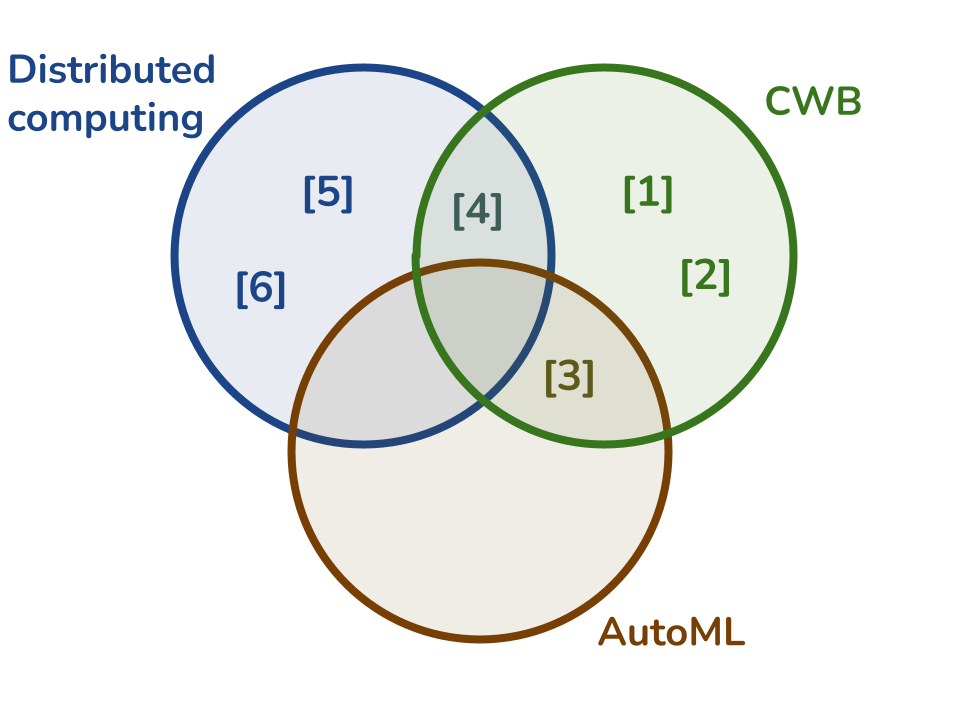
\includegraphics[width=0.55\textwidth]{figures/topics.png}
  \end{figure}
\end{frame}

\begin{frame}{Part I - Efficiency}
  \tikz[remember picture, overlay] \node[anchor=center] at ($(current page.center)-(-5,-2.5)$) {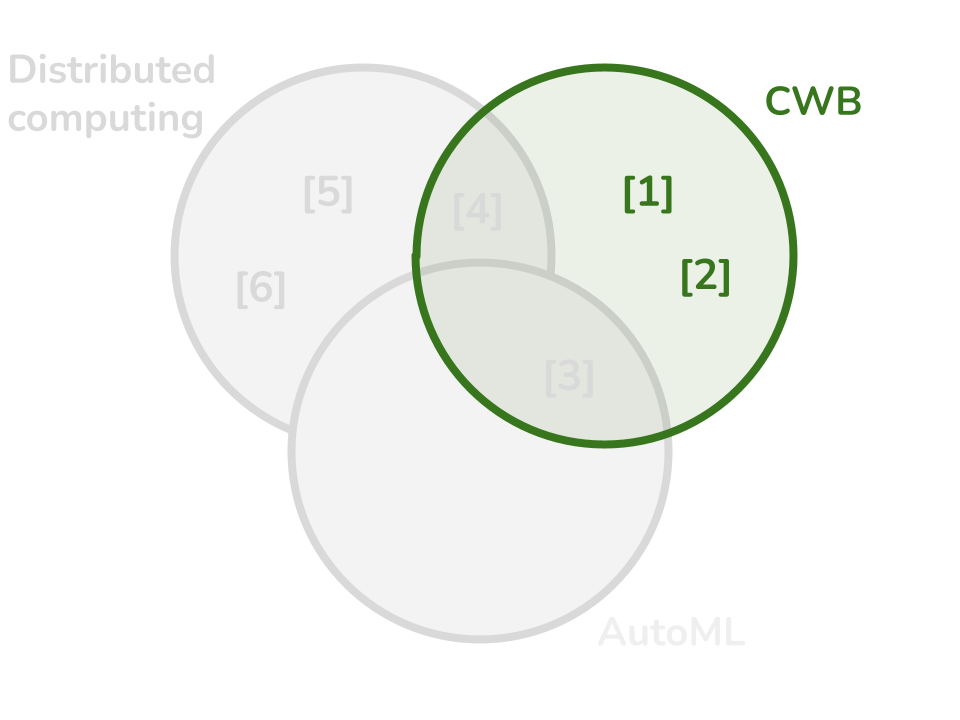
\includegraphics[width=0.3\textwidth]{figures/topics-cwb.png}};
  \begin{minipage}[t]{0.8\linewidth}
    \textbf{Goal:} Increase CWB's efficiency
    \begin{itemize}
      \item \textbf{Acceleration:} Speed up the fitting process by using Nesterovs momentum.
      \item \textbf{Memory:} Reduce the memory consumption by discretizing numerical features.
    \end{itemize}
  \end{minipage}
  \vspace{0.3cm}

  \textbf{Publications:}
  \renewcommand{\newblock}{\newblocknew}
  \begin{itemize}
    \item[{[}1{]}] {\footnotesize\bibentry{schalk2018compboost}}
    \item[{[}2{]}] {\footnotesize\bibentry{schalk2022accelerated}}
  \end{itemize}
  \renewcommand{\newblock}{\newblockold}
\end{frame}

\begin{frame}{Part II - Interpretable AutoML Framework}
  \tikz[remember picture, overlay] \node[anchor=center] at ($(current page.center)-(-5,-2.5)$) {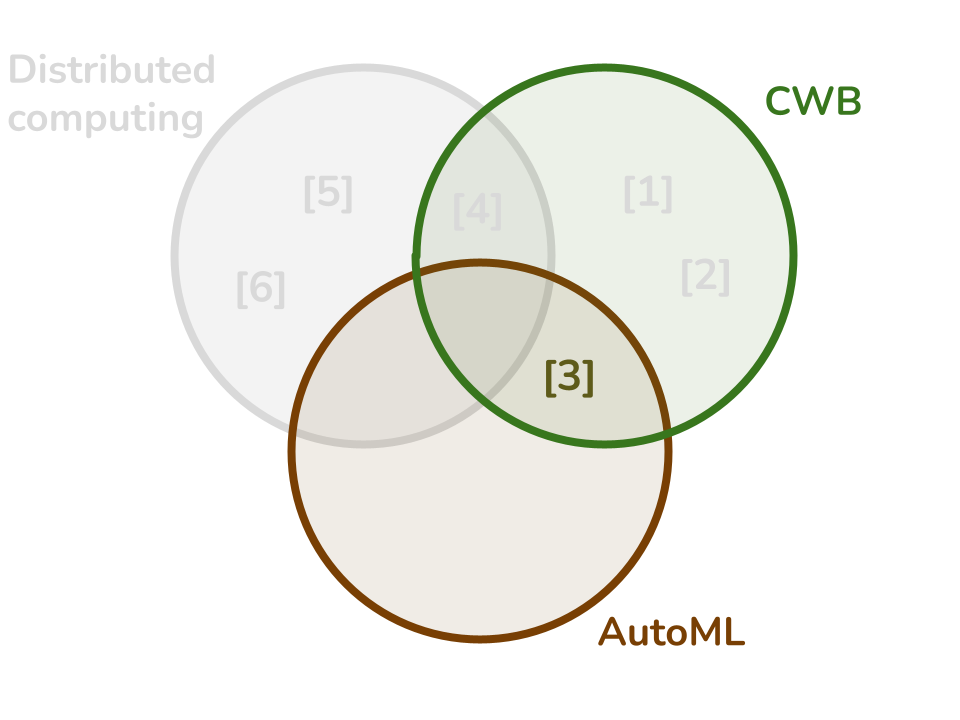
\includegraphics[width=0.3\textwidth]{figures/topics-autocwb.png}};
  \begin{minipage}[t]{0.8\linewidth}
    \textbf{Goal:}
    \begin{itemize}
      \item
        Easy access to an interpretable AutoML framework based on CWB as fitting engine.
      \item
        Focus is the assessment of the required complexity to model a given task.
    \end{itemize}
  \end{minipage}
  \vspace{0.3cm}

  \textbf{Publication:}
  \renewcommand{\newblock}{\newblocknew}
  \begin{itemize}
    \item[{[}3{]}] {\footnotesize\bibentry{coors2021autocompboost}}
  \end{itemize}
  \renewcommand{\newblock}{\newblockold}
\end{frame}

\begin{frame}{Part III - Distributed Computing}
  \tikz[remember picture, overlay] \node[anchor=center] at ($(current page.center)-(-5,-2.5)$) {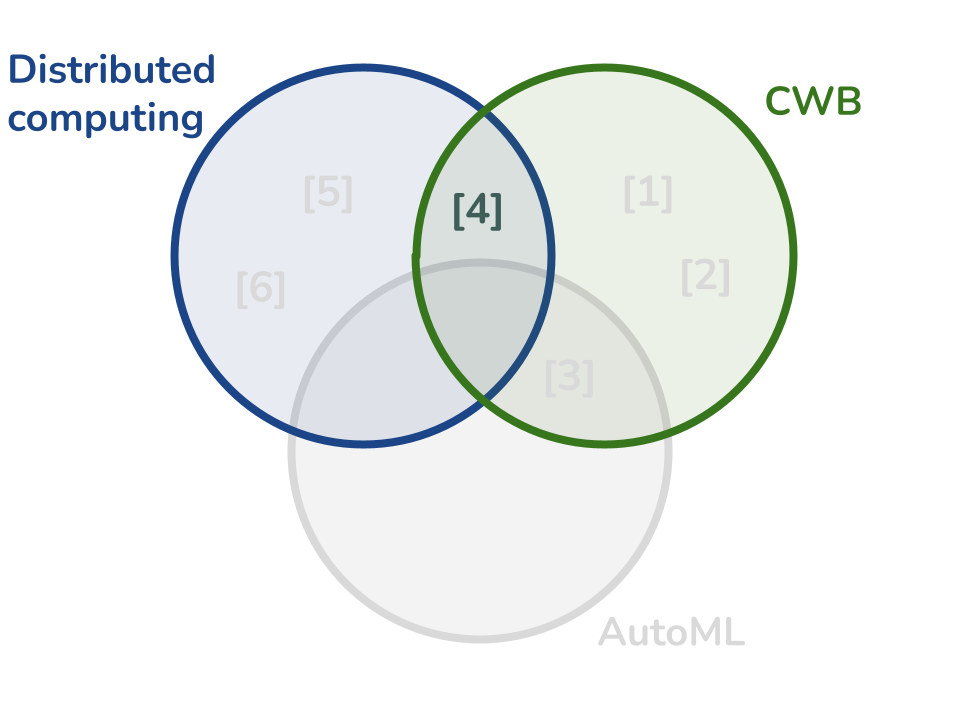
\includegraphics[width=0.3\textwidth]{figures/topics-dcwb.png}};
  \begin{minipage}[t]{0.8\linewidth}
    \textbf{Goal:}
    \begin{itemize}
      \item
        Distributed and privacy-preserving computation of CWB.
      \item
        Estimation of common shared effects and site-specific effect corrections.
    \end{itemize}
  \end{minipage}
  \vspace{0.3cm}

  \textbf{Publications:}
  \renewcommand{\newblock}{\newblocknew}
  \begin{itemize}
    \item[{[}4{]}] {\footnotesize\bibentry{schalk2022distcwb}. [Currently under review in the journal \textit{Statistics and Computing}]}
  \end{itemize}
  \renewcommand{\newblock}{\newblockold}

\end{frame}

\begin{frame}{Part III - Distributed Computing}
  \tikz[remember picture, overlay] \node[anchor=center] at ($(current page.center)-(-5,-2.5)$) {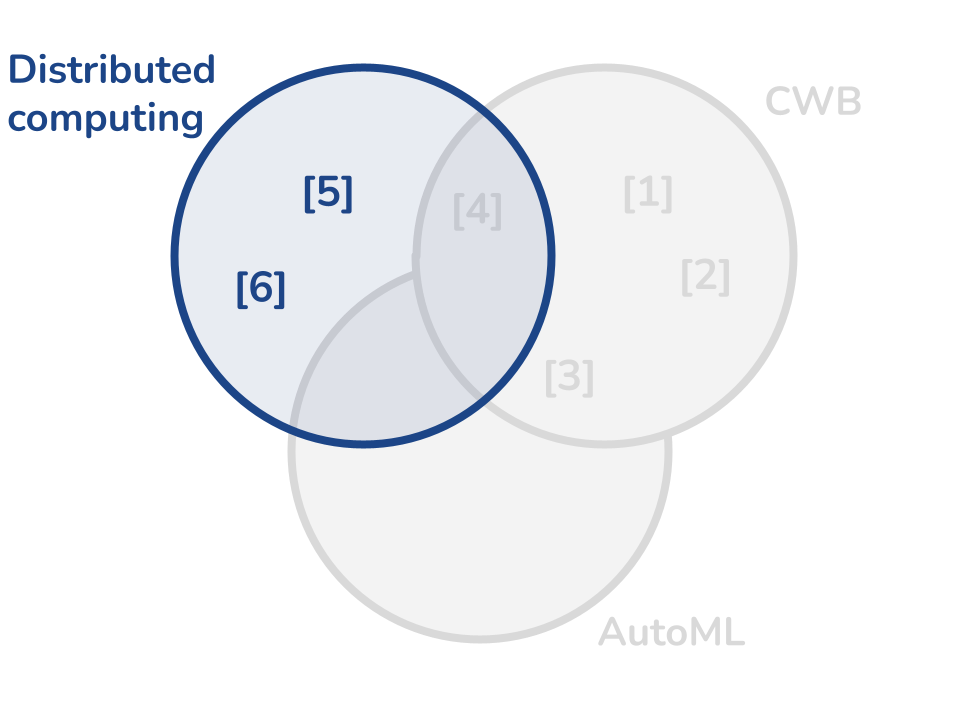
\includegraphics[width=0.3\textwidth]{figures/topics-dauc.png}};
  \begin{minipage}[t]{0.8\linewidth}
  \textbf{Goal:}
    \begin{itemize}
      \item
        Methodology and implementation of a distributed and privacy-preserving ROC analysis.
    \end{itemize}
  \end{minipage}
  \vspace{0.3cm}

  \textbf{Publications:}
  \renewcommand{\newblock}{\newblocknew}
  \begin{itemize}
    \item[{[}5{]}] {\footnotesize\bibentry{schalk2022dauc} [Currently under review in the journal \textit{BMC Medical Research Methodology}]}
    \item[{[}6{]}] {\footnotesize\bibentry{schalk2022dsBinVal}}
  \end{itemize}
  \renewcommand{\newblock}{\newblockold}

\end{frame}

\begin{frame}{Overview}
  \textbf{Contribution and topics:}
  \begin{figure}
    \centering
    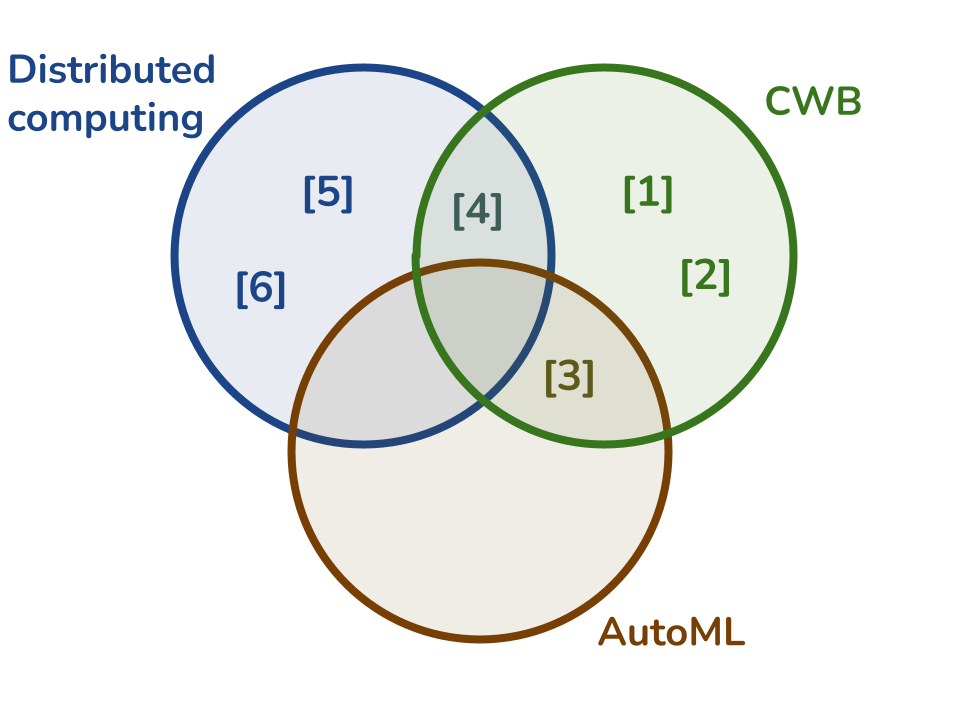
\includegraphics[width=0.55\textwidth]{figures/topics.png}
  \end{figure}\vspace{-0.2cm}
  The focus of this presentation is on CWB adjustments {[}1{]}, {[}2{]}, and {[}4{]}. The other contributions are briefly summarized at the end of the presentation.
\end{frame}

\begin{frame}{Overview}
  \textbf{Contribution and topics:}
  \begin{figure}
    \centering
    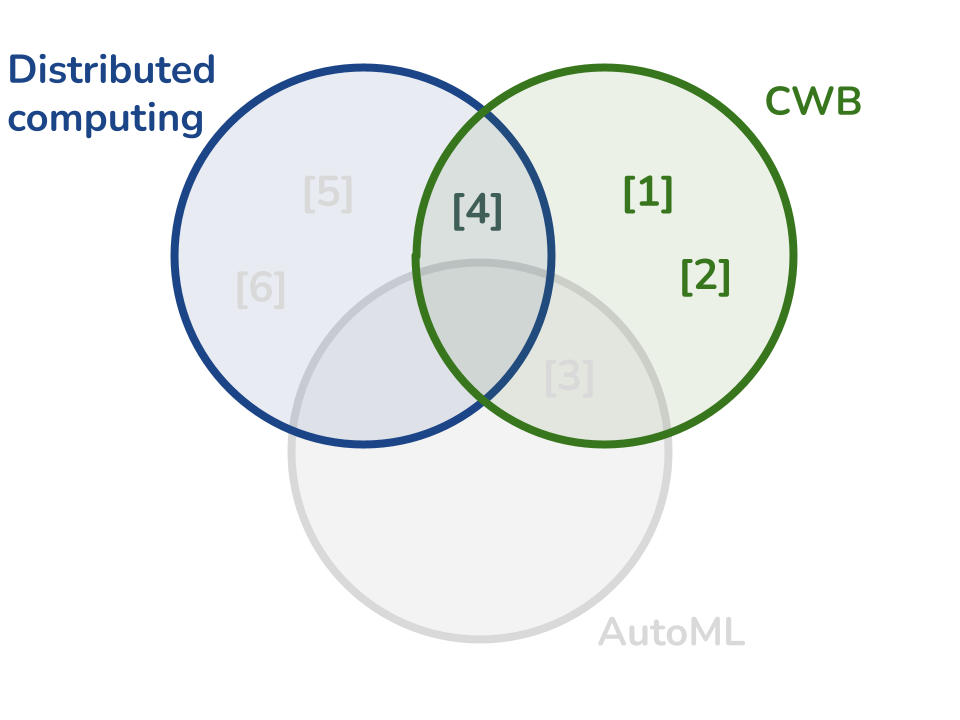
\includegraphics[width=0.55\textwidth]{figures/topics-relevant.png}
  \end{figure}\vspace{-0.2cm}
  The focus of this presentation is on CWB adjustments {[}1{]}, {[}2{]}, and {[}4{]}. The other contributions are briefly summarized at the end of the presentation.
	\addtocounter{framenumber}{-1}
\end{frame}


\begin{frame}{Structure of the talk}
  \tableofcontents
\end{frame}

\section{Background}

\begin{frame}{History of component-wise boosting}

\end{frame}

\begin{frame}{Terminology}
  \begin{itemize}

    \item
      $p$-dimensional covariate or feature vector $\xv = (x_1, \dots, x_p) \in \Xspace =  \Xspace_1 \times \cdots\times$ and target variable $y\in\Yspace$.

    \item
      Data set $\D = \Dset$ with $(\xi, \yi)$ sampled from an unknown probability distribution $\mathbb{P}_{xy}$.

    \item
      True underlying relationship $f : \Xspace^p \to \R$, $\xv \mapsto f(\xv)$.

    \item
      Goal of Machine Learning (ML) is to estimate a model $\fh = \argmin_{f} \riske(f | \D)$ with
      \begin{itemize}
        \item Empirical risk $\riske(f | \D) = n^{-1} \sum_{(\xv, y)\in\D} L(y, \fh(\xv))$ and
        \item Loss function $L : \Yspace\times\Yspace \to \R_+$, $(y,\yhat) \mapsto L(y,\yhat)$.
      \end{itemize}

    \item
      The inducer $\Ind : \mathbb{D} \times \hpspace \to \fspace$, $(\D, \hp) \mapsto \fh=\Ind_{\hp}(\D)$ gets a data set $\D\in\mathbb{D}$ with hyperparameters (HPs) $\hp\in\hpspace$.

  \end{itemize}
\end{frame}

\begin{frame}{Gradient boosting}
  \begin{itemize}
    \item
      Gradient boosting (GB) aims to estimate $f$ based on assembling weak base learners $b:\Xspace \to \Yspace, \xv \mapsto b(\xv | \tb)$ parameterized by $\tb$.

    \item
      The model estimate $\fh$ is fitted by conducting functional gradient descent $\fmdh = \fmh + \nu \hat{b}^{[m]}$ for $M$ steps. The estimated model is then $\fh = \fmh[M]$.

    \item
      To obtain the model update $\hat{b}^{[m]}$ in iteration $m$, the weak base learner $b$ is fit to pseudo residuals $\rmm$ by minimizing the SSE: $\tbmh = \argmin_{\tb} \sum_{i=1}^n(\rmi - b(\xi | \tb))^2$

    \item
      The pseudo residuals $\rmi = -\left.\pd{\Lxyi}{f(\xi)}\right|_{f = \fmdh}$, $i \in \{1, \dots, n\}$, ($\rmm$ is the vector of pseudo residuals) contain the information in which direction to move $\fmh$ for a better fit to the training data $\D$.

    \item
      The fitting is initialized with $\fh^{[0]}(\xv) = \argmin_{c\in\mathcal{Y}}\riske(c|\D)$ and repeated $M$ times or until an early stopping criterion is met.
  \end{itemize}
\end{frame}

\begin{frame}{Gradient boosting -- Algorithm}

  \begin{algorithm}[H]
  \footnotesize
  \caption{GB algorithm}\label{algo:gb}
  %\vspace{0.15cm}
  \hspace*{\algorithmicindent} \textbf{Input} Train data $\D$, number of boosting iterations $M$, loss function $L$, base learner $b$\\
  \hspace*{\algorithmicindent} \textbf{Output} Model $\fh = \fmh[M]$\vspace{0.1cm}
  \hrule
  \begin{algorithmic}[1]
  \Procedure{$\operatorname{GB}$}{$\D,M, L,b$}
      \State Initialize: $f_0 = \fh^{[0]}(\xv) = \argmin_{c\in\mathcal{Y}}\riske(c|\D)$
      \While{$m \leq M$}
          \State $\rmi = -\left.\pd{\Lxyi}{f(\xi)}\right|_{f = \fmdh},\ \ \forall i \in \{1, \dots, n\}$
          \State $\tbmh = \argmin_{\tb} \sum_{i=1}^n(\rmi - b(\xi | \tb))^2$
          \State $\nu_m = \argmin_{\nu\in\R} \sum_{i=1}^n L(\rmi, \fmh + \nu \hat{b}^{[m]}(\xi | \tbmh))$
          \State $\fmh(\xv) = \fmdh(\xv) + \nu_m \hat{b}^{[m]}(\xv | \tbmh)$
      \EndWhile
      \State \textbf{return} $\fh = \fh^{[M]}$
  \EndProcedure
  \end{algorithmic}
  \end{algorithm}
  \vspace{-0.5cm}
  Note: A common choice for the base learner in GB is, e.g., to use trees~\citep{friedman2001greedy}. Based on the base learner, further adaptions to the algorithm are made to, e.g., increase speed or predictive power~\citep{chen2015xgboost}.
\end{frame}

\fSlide{Background}{Component-wise gradient boosting}

\begin{frame}{Basics}
  \begin{itemize}
    \item
      Compared to GB, CWB can choose from a set of $K$ base learners $b \in \{b_1, \dots, b_K\}$.

    \item
      The learning rate $\nu$ is fixed and not optimized by a line search.

    \item
      Often, $b_1, \dots, b_K$ are chosen to be (interpretable) statistical models and hence $f$ corresponds to a generalized additive model~\citep[GAM;][]{hastie2017generalized}: \[f(\xv) = f_0 + \sum_{k=1}^K b_k(\xv), \ \ \text{intercept}\ f_0\]

    \item
      Advantages of CWB:
      \begin{itemize}
        \item
          Feasible to get fit in high-dimensional feature spaces ($p \gg n$).

        \item
          An inherent (unbiased) feature selection.

        \item
          Interpretable/explainable partial feature effects (depending on the choice of base learners).
      \end{itemize}
  \end{itemize}
\end{frame}

\begin{frame}{Base learner}
  \begin{itemize}
    \item
      From now on, each base learner $b_k$ is defined by a basis transformation $g_k : \Xspace \to \R^{d_k}$ with $g_k(\xv) = (g_{k,1}(\xv), \dots, g_{k,d_k}(\xv))^\tran$.

    \item
      The base learners are also restricted to be linear in the parameters: $b_k(\xv | \tb) = g_k(\xv)^\tran \tb$

    \item
      Due to the linearity, the sum of two base learners $b_k(\xv | \tb_l) + b_k(\xv | \tb_m)$ equals $b_k(\xv | \tb_l + \tb_m)$.

    \item
      For $n$ data points $\xi[1], \dots, \xi[n]$, each base learner defines a design matrix $\design_k = (g_k(\xi[1])^\tran, \dots, g_k(\xi[n])^\tran)^\tran\in\R^{n\times d_k}$.

    \item
      Based on the linearity and the design matrix, each base learner can be fitted by calculating the least squares estimator $\tbh_k = (\design_\blk^\tran \design_\blk) \design_k^\tran \yv$.

    \item
      Further, a base learner is allowed to include a penalization defined by a matrix $\bm{K}_k$ which extends the estimation to $\tbh_k = (\design_\blk^\tran \design_\blk + \bm{K}_k) \design_k^\tran \yv$.

  \end{itemize}
\end{frame}

\begin{frame}{Algorithm}

  \begin{algorithm}[H]
  \footnotesize
  \caption{Vanilla CWB algorithm}\label{algo:cwb}
  %\vspace{0.15cm}
  \hspace*{\algorithmicindent} \textbf{Input} Train data $\D$, learning rate $\nu$, number of boosting iterations $M$, loss\\
  \hspace*{\algorithmicindent} \phantom{\textbf{Input} } function $L$, base learners $b_1, \dots, b_\blK$\\
  \hspace*{\algorithmicindent} \textbf{Output} Model $\fh = \fmh[M]$\vspace{0.1cm}
  \hrule
  \begin{algorithmic}[1]
  \Procedure{$\operatorname{CWB}$}{$\D,\nu,M,L,b_1, \dots, b_\blK$}
      \State \tikzmk{A}Initialize: $f_0 = \fh^{[0]}(\xv) = \argmin_{c\in\mathcal{Y}}\riske(c|\D)$
      \While{$m \leq M$}
          \State $\rmi = -\left.\pd{\Lxyi}{f(\xi)}\right|_{f = \fmdh},\ \ \forall i \in \{1, \dots, n\}$\tikzmk{B}\boxtrans
          \For{\tikzmk{A}$\blk \in \{1, \dots, \blK\}$}
              \State $\tbmh_\blk = \left(\design_\blk^\tran \design_\blk + \bm{K}_\blk\right)^{-1} \design^\tran_\blk \rmm$
              \State $\sse_\blk = \sum_{i=1}^n(\rmi - b_\blk(\xi | \tbmh_\blk))^2$
          \EndFor
          \State $\blk^{[m]} = \argmin_{\blk\in\{1, \dots, \blK\}} \sse_\blk$
          \tikzmk{B}
          \boxit{olivedrab}
          \State \tikzmk{A}$\fmh(\xv) = \fmdh(\xv) + \nu b_{\blk^{[m]}} (\xv | \tbmh_{\blk^{[m]}})$\tikzmk{B}\boxtrans
      \EndWhile
      \State \textbf{return} $\fh = \fh^{[M]}$
  \EndProcedure
  \end{algorithmic}
  \end{algorithm}
\end{frame}

\begin{frame}{Initialization vs. fitting phase}
  \textbf{Initialization:}
  \begin{itemize}
    \item
      All design matrices $\design_k$ and penalties $\penMat_k$ are calculated for $k = 1, \dots, K$ and stored.
    \item
      Additionally, the Cholesky decomposition $\bm{L}_k$ of $\design_k^\tran \design_k + \penMat_k$ is calculated and stored.
  \end{itemize}
  \textbf{Fitting:}
  \begin{itemize}
    \item
      Algorithm~\ref{algo:cwb} is executed.
    \item
      But, instead of calculating $\tbmh_\blk = \left(\design_\blk^\tran \design_\blk + \bm{K}_\blk\right)^{-1} \design^\tran_\blk \rmm$ in each iteration, reuse $\bm{L}_k$ to calculate $\tbmh$.
  \end{itemize}

\end{frame}


\begin{frame}{Example data}
  Example throughout this presentation is a subset of a WHO data set\footnote[frame,1]{Available at \url{kaggle.com/datasets/kumarajarshi/life-expectancy-who}} about life expectation in years per country:

  \scriptsize
  \begin{table}
\centering
\begin{tabular}[t]{rlrrr}
\toprule
\textbf{Life.expectancy} & \textbf{Country} & \textbf{Year} & \textbf{BMI} & \textbf{Adult.Mortality}\\
\midrule
\cellcolor{gray!6}{53.2} & \cellcolor{gray!6}{ETH} & \cellcolor{gray!6}{2002} & \cellcolor{gray!6}{12.9} & \cellcolor{gray!6}{369}\\
81.0 & GER & 2015 & 62.3 & 68\\
\cellcolor{gray!6}{76.8} & \cellcolor{gray!6}{USA} & \cellcolor{gray!6}{2000} & \cellcolor{gray!6}{6.1} & \cellcolor{gray!6}{114}\\
79.1 & USA & 2014 & 69.1 & 14\\
\cellcolor{gray!6}{58.9} & \cellcolor{gray!6}{ZAF} & \cellcolor{gray!6}{2011} & \cellcolor{gray!6}{47.9} & \cellcolor{gray!6}{413}\\
69.0 & ZAF & 2013 & 49.5 & 371\\
\bottomrule
\end{tabular}
\end{table}

  \normalsize

\end{frame}

%\begin{frame}{Component-wise gradient boosting – Example}
%  Example throughout this presentation is a subset of a WHO data set\footnote[frame,1]{Full description and data is available at \url{kaggle.com/datasets/kumarajarshi/life-expectancy-who}} about life expectation in years per country:
%
%  \begin{itemize}
%    \item
%      Target variable is \texttt{Life.expectancy} in years.
%    \item
%      Features are \texttt{Country}, \texttt{Year}, \texttt{Alcohol} recorded per capital (15+) consumption (in liters of pure alcohol), and \texttt{Adult.Mortality} rates of both sexes of dying between 15 and 60 years per 1000 population.
%
%    \item
%      Numerical features \texttt{Year}, \texttt{Alcohol} and \texttt{Adult.Mortality} are modeled as P-splines \citep{eilers1996flexible} and \texttt{Country} as one-hot-encoded linear model with ridge penalty.
%
%    %\item
%      %Define setup, iterations etc.
%  \end{itemize}
%\end{frame}

\fSlide{Component-wise gradient boosting}{Base learner}

\begin{frame}{B/P-Spline base learner}
  \vspace{-0.3cm}\[g_k(x) = (B_{k,1}(x), \dots, B_{k,d_k}(x))^\tran\] B-spline basis $B$ of a pre-defined degree~\citep{eilers1996flexible}.
  \begin{center}
    \begin{figure}
      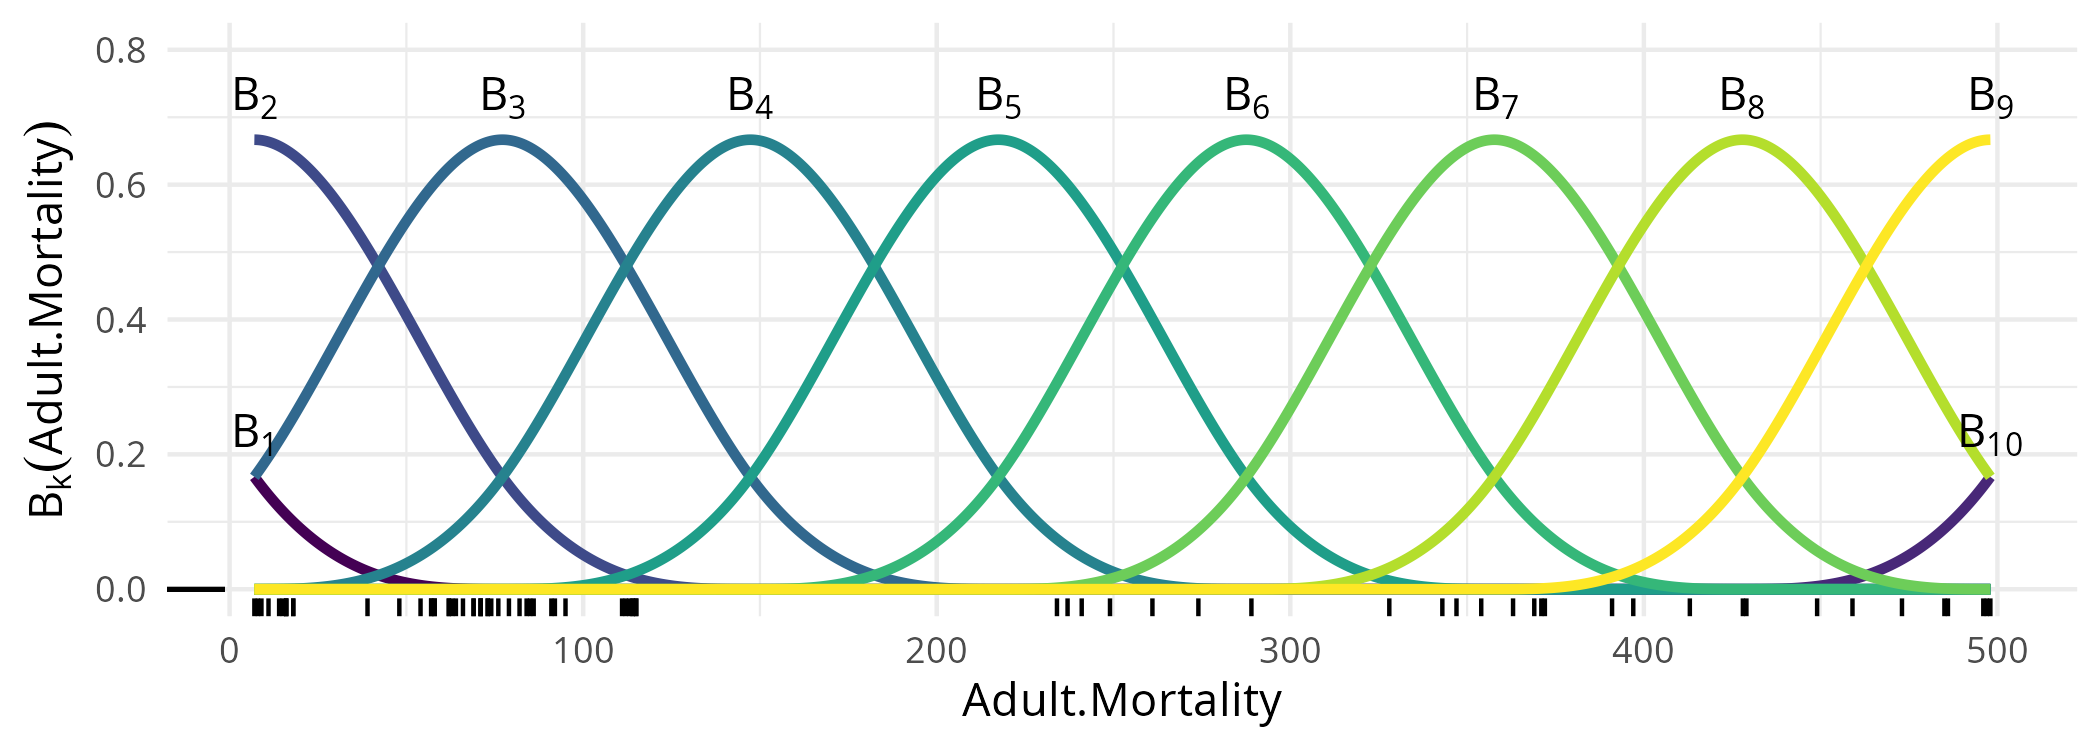
\includegraphics[width=0.7\textwidth]{figures/bs-base/fig-bs0.png}
    \end{figure}
    \vspace{-0.3cm}
    \[
    \design_k = \left(\begin{array}{c}
      g_{k}^\tran(\xi[1]) \\
      \vdots \\
      g_{k}^\tran(\xi[n])
    \end{array}\right) = \left(\begin{array}{ccc}
      B_{k,1}(\xi[1]) & \dots & B_{k,d_k}(\xi[1]) \\
      \vdots &  & \vdots \\
      B_{k,1}(\xi[n]) & \dots & B_{k,d_k}(\xi[n])
    \end{array}\right)\in\R^{n\times d_k}
    \]
  \end{center}

\end{frame}


\begin{frame}{B/P-spline base learner}
  \vspace{-0.3cm}\[g_k(x) = (B_{k,1}(x), \dots, B_{k,d_k}(x))^\tran\] B-spline basis $B$ of a pre-defined degree~\citep{eilers1996flexible}.
  \begin{center}
    \begin{figure}
      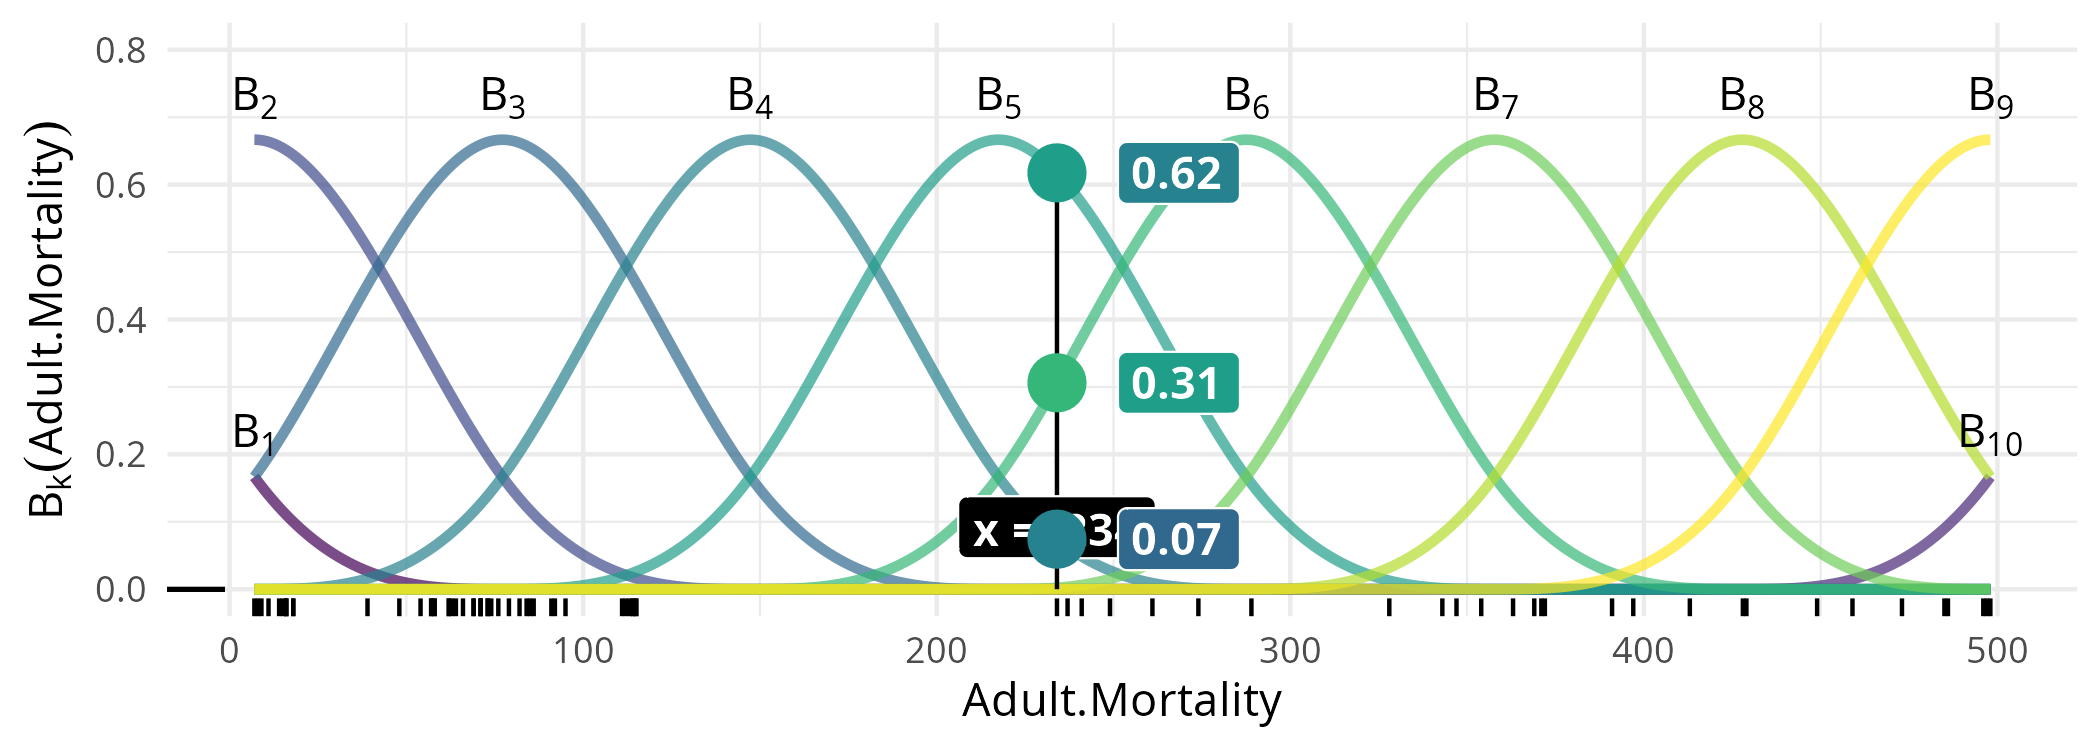
\includegraphics[width=0.7\textwidth]{figures/bs-base/fig-bs1.png}
    \end{figure}
  \end{center}
  \vspace{-0.3cm}
  
\[
\design_k = \tiny\begin{blockarray}{cccccccccc}
\color[HTML]{440154}B_{1} & \color[HTML]{482878}B_{2} & \color[HTML]{3E4A89}B_{3} & \color[HTML]{31688E}B_{4} & \color[HTML]{26828E}B_{5} & \color[HTML]{1F9E89}B_{6} & \color[HTML]{35B779}B_{7} & \color[HTML]{6DCD59}B_{8} & \color[HTML]{B4DE2C}B_{9} & \color[HTML]{FDE725}B_{10} \\
\begin{block}{(cccccccccc)}
\phantom{x}\\
\color{lightgray}0.00 & \color{lightgray}0.00 & \color{lightgray}0.00 & \color[HTML]{31688E}0.07 & \color[HTML]{26828E}0.62 & \color[HTML]{1F9E89}0.31 & \color{lightgray}0.00 & \color{lightgray}0.00 & \color{lightgray}0.00 & \color{lightgray}0.00\color{black}\\
\end{block}
\color{white}0.00 & \color{white}0.20 & \color{white}0.66 & \color{white}0.14 & \color{white}0.00 & \color{white}0.00 & \color{white}0.00 & \color{white}0.00 & \color{white}0.00 & \color{white}0.00\color{black}\\
  \color{white}0.00 & \color{white}0.00 & \color{white}0.00 & \color{white}0.00 & \color{white}0.00 & \color{white}0.00 & \color{white}0.00 & \color{white}0.17 & \color{white}0.67 & \color{white}0.17\color{black}\\
  \color{white}\vdots & \color{white}\vdots & \color{white}\vdots & \color{white}\vdots & \color{white}\vdots & \color{white}\vdots & \color{white}\vdots & \color{white}\vdots & \color{white}\vdots & \color{white}\vdots\\
  \color{white}0.00 & \color{white}0.02 & \color{white}0.48 & \color{white}0.48 & \color{white}0.02 & \color{white}0.00 & \color{white}0.00 & \color{white}0.00 & \color{white}0.00 & \color{white}0.00\color{black}\\
  \color{white}0.00 & \color{white}0.00 & \color{white}0.00 & \color{white}0.01 & \color{white}0.40 & \color{white}0.55 & \color{white}0.04 & \color{white}0.00 & \color{white}0.00 & \color{white}0.00\color{black}\\
  \color{white}0.00 & \color{white}0.00 & \color{white}0.00 & \color{white}0.00 & \color{white}0.00 & \color{white}0.29 & \color{white}0.63 & \color{white}0.08 & \color{white}0.00 & \color{white}0.00\color{black}\\
\phantom{x}
\end{blockarray}
\]
\normalsize

  
\end{frame}


\begin{frame}{B/P-spline base learner}
  \vspace{-0.3cm}\[g_k(x) = (B_{k,1}(x), \dots, B_{k,d_k}(x))^\tran\] B-spline basis $B$ of a pre-defined degree~\citep{eilers1996flexible}.
  \begin{center}
    \begin{figure}
      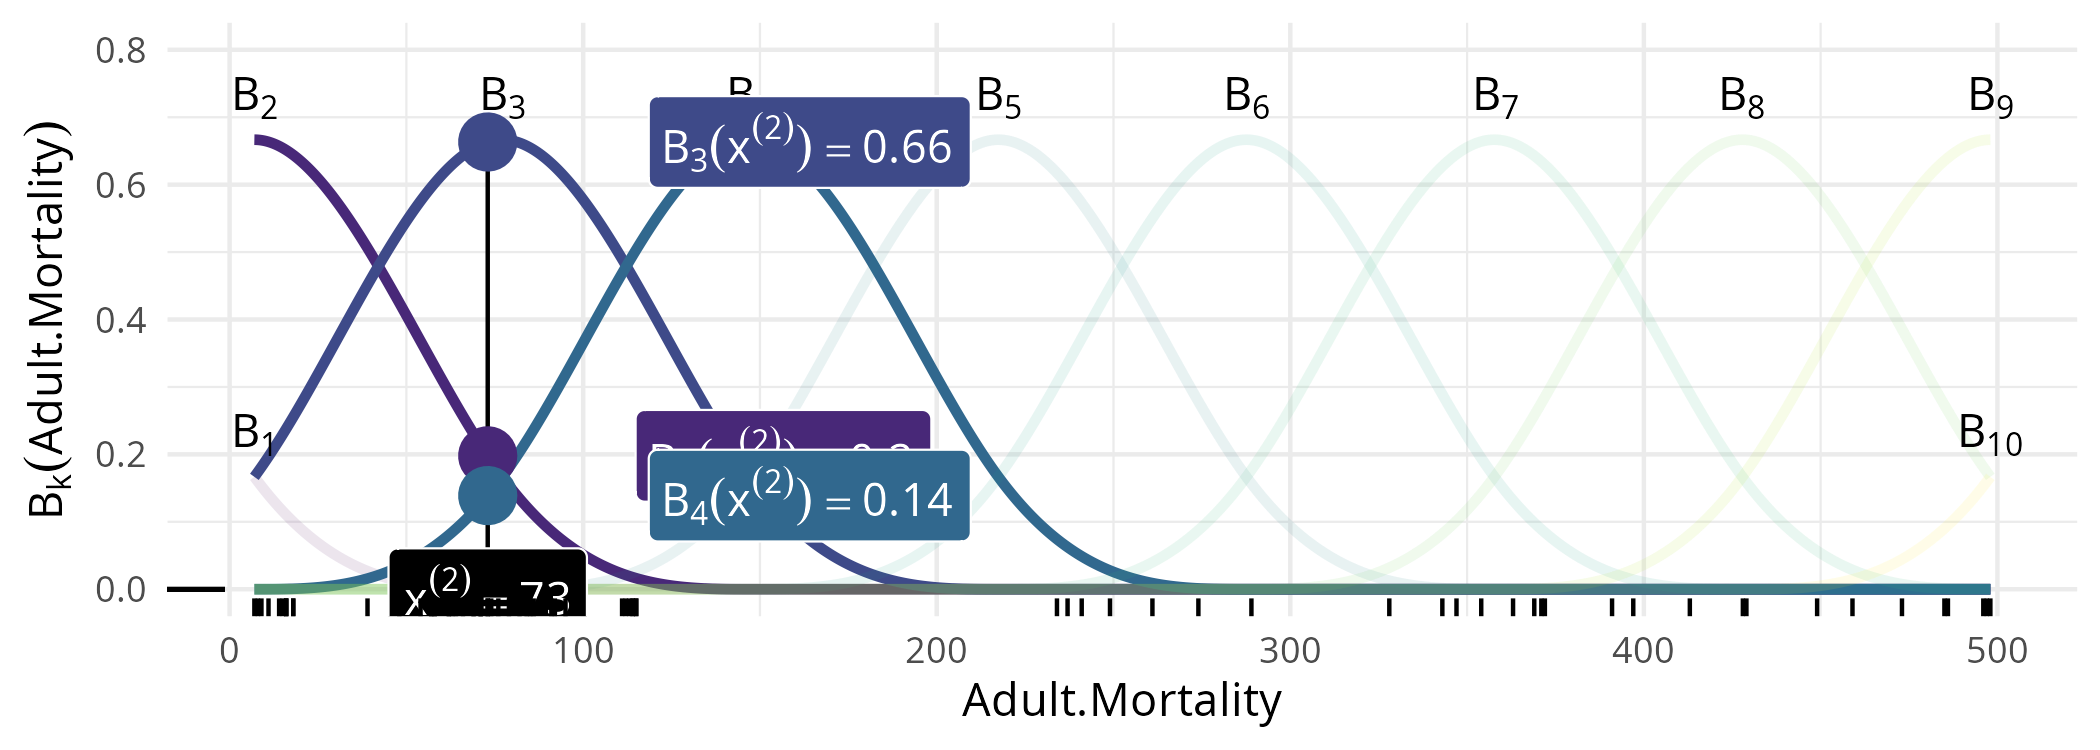
\includegraphics[width=0.7\textwidth]{figures/bs-base/fig-bs59.png}
    \end{figure}
  \end{center}
  \vspace{-0.3cm}
  \[
\design_k = \tiny\begin{blockarray}{cccccccccc}
\color[HTML]{440154}B_{1} & \color[HTML]{482878}B_{2} & \color[HTML]{3E4A89}B_{3} & \color[HTML]{31688E}B_{4} & \color[HTML]{26828E}B_{5} & \color[HTML]{1F9E89}B_{6} & \color[HTML]{35B779}B_{7} & \color[HTML]{6DCD59}B_{8} & \color[HTML]{B4DE2C}B_{9} & \color[HTML]{FDE725}B_{10} \\
\begin{block}{(cccccccccc)}
\phantom{x}\\
\color{lightgray}0.00 & \color{lightgray}0.00 & \color{lightgray}0.00 & \color{gray}0.07 & \color{gray}0.62 & \color{gray}0.31 & \color{lightgray}0.00 & \color{lightgray}0.00 & \color{lightgray}0.00 & \color{lightgray}0.00\color{black}\\
  \color{lightgray}0.00 & \color[HTML]{482878}0.20 & \color[HTML]{3E4A89}0.66 & \color[HTML]{31688E}0.14 & \color{lightgray}0.00 & \color{lightgray}0.00 & \color{lightgray}0.00 & \color{lightgray}0.00 & \color{lightgray}0.00 & \color{lightgray}0.00\color{black}\\
\color{white}0.00 & \color{white}0.00 & \color{white}0.00 & \color{white}0.00 & \color{white}0.00 & \color{white}0.00 & \color{white}0.00 & \color{white}0.17 & \color{white}0.67 & \color{white}0.17\color{black}\\
  \color{white}\vdots & \color{white}\vdots & \color{white}\vdots & \color{white}\vdots & \color{white}\vdots & \color{white}\vdots & \color{white}\vdots & \color{white}\vdots & \color{white}\vdots & \color{white}\vdots\\
  \color{white}0.00 & \color{white}0.02 & \color{white}0.48 & \color{white}0.48 & \color{white}0.02 & \color{white}0.00 & \color{white}0.00 & \color{white}0.00 & \color{white}0.00 & \color{white}0.00\color{black}\\
  \color{white}0.00 & \color{white}0.00 & \color{white}0.00 & \color{white}0.01 & \color{white}0.40 & \color{white}0.55 & \color{white}0.04 & \color{white}0.00 & \color{white}0.00 & \color{white}0.00\color{black}\\
  \color{white}0.00 & \color{white}0.00 & \color{white}0.00 & \color{white}0.00 & \color{white}0.00 & \color{white}0.29 & \color{white}0.63 & \color{white}0.08 & \color{white}0.00 & \color{white}0.00\color{black}\\
\phantom{x}\\
\end{block}
\end{blockarray}
\]
\normalsize

  \addtocounter{framenumber}{-1}
\end{frame}


\begin{frame}{B/P-spline base learner}
  \vspace{-0.3cm}\[g_k(x) = (B_{k,1}(x), \dots, B_{k,d_k}(x))^\tran\] B-spline basis $B$ of a pre-defined degree~\citep{eilers1996flexible}.
  \begin{center}
    \begin{figure}
      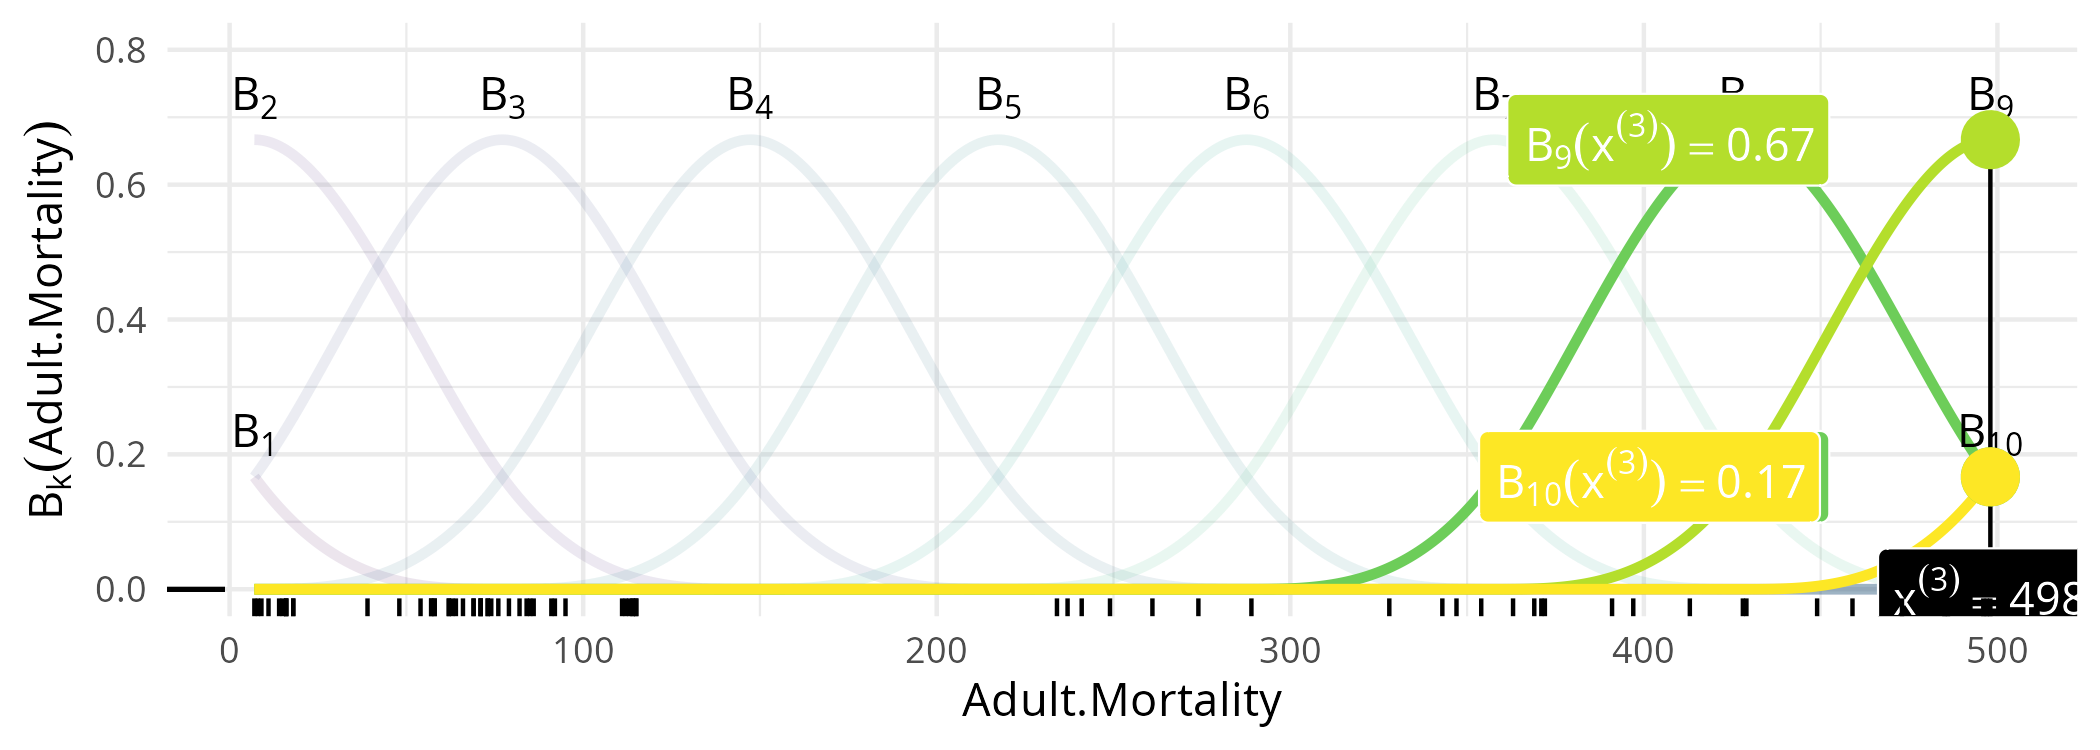
\includegraphics[width=0.7\textwidth]{figures/bs-base/fig-bs40.png}
    \end{figure}
  \end{center}
  \vspace{-0.3cm}
  \scriptsize
$$
\design_k = \begin{blockarray}{cccccccccc}
\color[HTML]{440154}B_{1} & \color[HTML]{482878}B_{2} & \color[HTML]{3E4A89}B_{3} & \color[HTML]{31688E}B_{4} & \color[HTML]{26828E}B_{5} & \color[HTML]{1F9E89}B_{6} & \color[HTML]{35B779}B_{7} & \color[HTML]{6DCD59}B_{8} & \color[HTML]{B4DE2C}B_{9} & \color[HTML]{FDE725}B_{10} \\
\begin{block}{(cccccccccc)}
\color{lightgray}0.00 & \color{lightgray}0.00 & \color{lightgray}0.00 & \color{gray}0.07 & \color{gray}0.62 & \color{gray}0.31 & \color{lightgray}0.00 & \color{lightgray}0.00 & \color{lightgray}0.00 & \color{lightgray}0.00\color{black}\\
  \color{lightgray}0.00 & \color{gray}0.20 & \color{gray}0.66 & \color{gray}0.14 & \color{lightgray}0.00 & \color{lightgray}0.00 & \color{lightgray}0.00 & \color{lightgray}0.00 & \color{lightgray}0.00 & \color{lightgray}0.00\color{black}\\
  \color{lightgray}0.00 & \color{lightgray}0.00 & \color{lightgray}0.00 & \color{lightgray}0.00 & \color{lightgray}0.00 & \color{lightgray}0.00 & \color{lightgray}0.00 & \color[HTML]{6DCD59}0.17 & \color[HTML]{B4DE2C}0.67 & \color[HTML]{FDE725}0.17\color{black}\\
  \color{white}\vdots & \color{white}\vdots & \color{white}\vdots & \color{white}\vdots & \color{white}\vdots & \color{white}\vdots & \color{white}\vdots & \color{white}\vdots & \color{white}\vdots & \color{white}\vdots\\
  
\end{block}
\color{white}0.00 & \color{white}0.02 & \color{white}0.48 & \color{white}0.48 & \color{white}0.02 & \color{white}0.00 & \color{white}0.00 & \color{white}0.00 & \color{white}0.00 & \color{white}0.00\color{black}\\
  \color{white}0.00 & \color{white}0.00 & \color{white}0.00 & \color{white}0.01 & \color{white}0.40 & \color{white}0.55 & \color{white}0.04 & \color{white}0.00 & \color{white}0.00 & \color{white}0.00\color{black}\\
  \color{white}0.00 & \color{white}0.00 & \color{white}0.00 & \color{white}0.00 & \color{white}0.00 & \color{white}0.29 & \color{white}0.63 & \color{white}0.08 & \color{white}0.00 & \color{white}0.00\color{black}
\end{blockarray}
$$
\normalsize

  \addtocounter{framenumber}{-1}
\end{frame}


\begin{frame}{B/P-spline base learner}
  \vspace{-0.3cm}\[g_k(x) = (B_{k,1}(x), \dots, B_{k,d_k}(x))^\tran\] B-spline basis $B$ of a pre-defined degree~\citep{eilers1996flexible}.
  \begin{center}
    \begin{figure}
      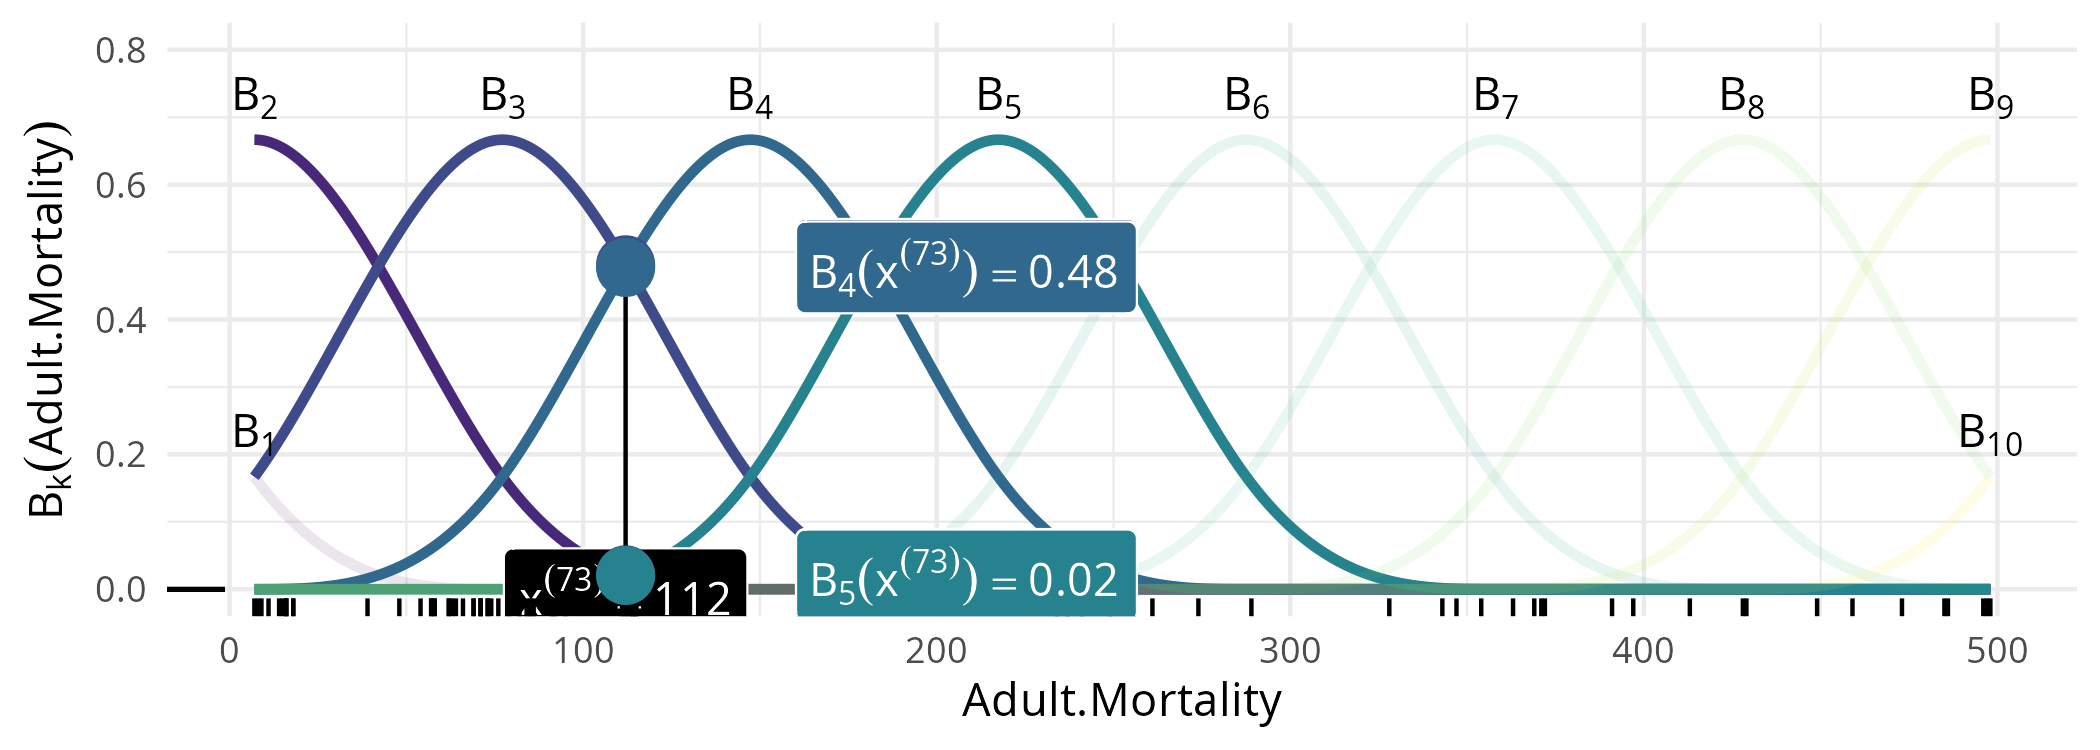
\includegraphics[width=0.7\textwidth]{figures/bs-base/fig-bs70.png}
    \end{figure}
  \end{center}
  \vspace{-0.3cm}
  \[
\design_k = \tiny\begin{blockarray}{cccccccccc}
\color[HTML]{440154}B_{1} & \color[HTML]{482878}B_{2} & \color[HTML]{3E4A89}B_{3} & \color[HTML]{31688E}B_{4} & \color[HTML]{26828E}B_{5} & \color[HTML]{1F9E89}B_{6} & \color[HTML]{35B779}B_{7} & \color[HTML]{6DCD59}B_{8} & \color[HTML]{B4DE2C}B_{9} & \color[HTML]{FDE725}B_{10} \\
\begin{block}{(cccccccccc)}
\phantom{x}\\
\color{lightgray}0.00 & \color{lightgray}0.00 & \color{lightgray}0.00 & \color{gray}0.07 & \color{gray}0.62 & \color{gray}0.31 & \color{lightgray}0.00 & \color{lightgray}0.00 & \color{lightgray}0.00 & \color{lightgray}0.00\color{black}\\
  \color{lightgray}0.00 & \color{gray}0.20 & \color{gray}0.66 & \color{gray}0.14 & \color{lightgray}0.00 & \color{lightgray}0.00 & \color{lightgray}0.00 & \color{lightgray}0.00 & \color{lightgray}0.00 & \color{lightgray}0.00\color{black}\\
  \color{lightgray}0.00 & \color{lightgray}0.00 & \color{lightgray}0.00 & \color{lightgray}0.00 & \color{lightgray}0.00 & \color{lightgray}0.00 & \color{lightgray}0.00 & \color{gray}0.17 & \color{gray}0.67 & \color{gray}0.17\color{black}\\
  \color{black}\vdots & \color{black}\vdots & \color{black}\vdots & \color{black}\vdots & \color{black}\vdots & \color{black}\vdots & \color{black}\vdots & \color{black}\vdots & \color{black}\vdots & \color{black}\vdots\\
  \color{lightgray}0.00 & \color[HTML]{482878}0.02 & \color[HTML]{3E4A89}0.48 & \color[HTML]{31688E}0.48 & \color[HTML]{26828E}0.02 & \color{lightgray}0.00 & \color{lightgray}0.00 & \color{lightgray}0.00 & \color{lightgray}0.00 & \color{lightgray}0.00\color{black}\\
\color{white}0.00 & \color{white}0.00 & \color{white}0.00 & \color{white}0.01 & \color{white}0.40 & \color{white}0.55 & \color{white}0.04 & \color{white}0.00 & \color{white}0.00 & \color{white}0.00\color{black}\\
  \color{white}0.00 & \color{white}0.00 & \color{white}0.00 & \color{white}0.00 & \color{white}0.00 & \color{white}0.29 & \color{white}0.63 & \color{white}0.08 & \color{white}0.00 & \color{white}0.00\color{black}\\
\phantom{x}\\
\end{block}
\end{blockarray}
\]
\normalsize

  \addtocounter{framenumber}{-1}
\end{frame}


\begin{frame}{B/P-spline base learner}
  \vspace{-0.3cm}\[g_k(x) = (B_{k,1}(x), \dots, B_{k,d_k}(x))^\tran\] B-spline basis $B$ of a pre-defined degree~\citep{eilers1996flexible}.
  \begin{center}
    \begin{figure}
      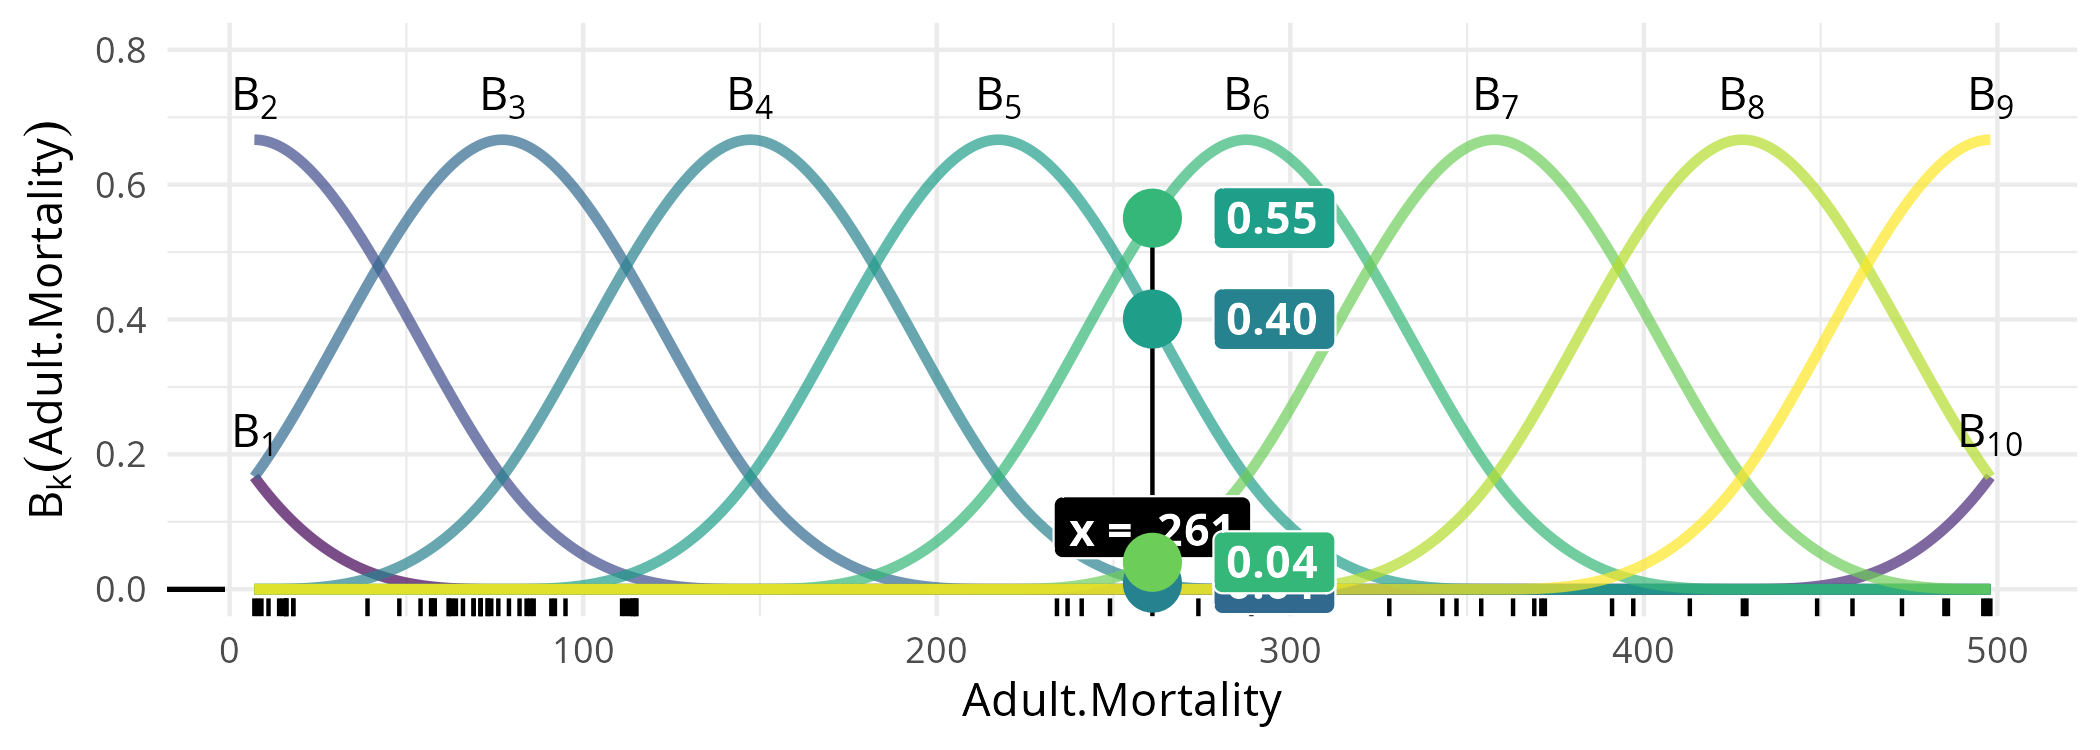
\includegraphics[width=0.7\textwidth]{figures/bs-base/fig-bs5.png}
    \end{figure}
  \end{center}
  \vspace{-0.3cm}
  \[
\design_k = \tiny\begin{blockarray}{cccccccccc}
\color[HTML]{440154}B_{1} & \color[HTML]{482878}B_{2} & \color[HTML]{3E4A89}B_{3} & \color[HTML]{31688E}B_{4} & \color[HTML]{26828E}B_{5} & \color[HTML]{1F9E89}B_{6} & \color[HTML]{35B779}B_{7} & \color[HTML]{6DCD59}B_{8} & \color[HTML]{B4DE2C}B_{9} & \color[HTML]{FDE725}B_{10} \\
\begin{block}{(cccccccccc)}
\phantom{x}\\
\color{lightgray}0.00 & \color{lightgray}0.00 & \color{lightgray}0.00 & \color{gray}0.07 & \color{gray}0.62 & \color{gray}0.31 & \color{lightgray}0.00 & \color{lightgray}0.00 & \color{lightgray}0.00 & \color{lightgray}0.00\color{black}\\
  \color{lightgray}0.00 & \color{gray}0.20 & \color{gray}0.66 & \color{gray}0.14 & \color{lightgray}0.00 & \color{lightgray}0.00 & \color{lightgray}0.00 & \color{lightgray}0.00 & \color{lightgray}0.00 & \color{lightgray}0.00\color{black}\\
  \color{lightgray}0.00 & \color{lightgray}0.00 & \color{lightgray}0.00 & \color{lightgray}0.00 & \color{lightgray}0.00 & \color{lightgray}0.00 & \color{lightgray}0.00 & \color{gray}0.17 & \color{gray}0.67 & \color{gray}0.17\color{black}\\
  \color{black}\vdots & \color{black}\vdots & \color{black}\vdots & \color{black}\vdots & \color{black}\vdots & \color{black}\vdots & \color{black}\vdots & \color{black}\vdots & \color{black}\vdots & \color{black}\vdots\\
  \color{lightgray}0.00 & \color{gray}0.02 & \color{gray}0.48 & \color{gray}0.48 & \color{gray}0.02 & \color{lightgray}0.00 & \color{lightgray}0.00 & \color{lightgray}0.00 & \color{lightgray}0.00 & \color{lightgray}0.00\color{black}\\
  \color{lightgray}0.00 & \color{lightgray}0.00 & \color{lightgray}0.00 & \color[HTML]{31688E}0.01 & \color[HTML]{26828E}0.40 & \color[HTML]{1F9E89}0.55 & \color[HTML]{35B779}0.04 & \color{lightgray}0.00 & \color{lightgray}0.00 & \color{lightgray}0.00\color{black}\\
\color{white}0.00 & \color{white}0.00 & \color{white}0.00 & \color{white}0.00 & \color{white}0.00 & \color{white}0.29 & \color{white}0.63 & \color{white}0.08 & \color{white}0.00 & \color{white}0.00\color{black}\\
\phantom{x}\\
\end{block}
\end{blockarray}
\]
\normalsize

  \addtocounter{framenumber}{-1}
\end{frame}


\begin{frame}{B/P-spline base learner}
  \vspace{-0.3cm}\[g_k(x) = (B_{k,1}(x), \dots, B_{k,d_k}(x))^\tran\] B-spline basis $B$ of a pre-defined degree~\citep{eilers1996flexible}.
  \begin{center}
    \begin{figure}
      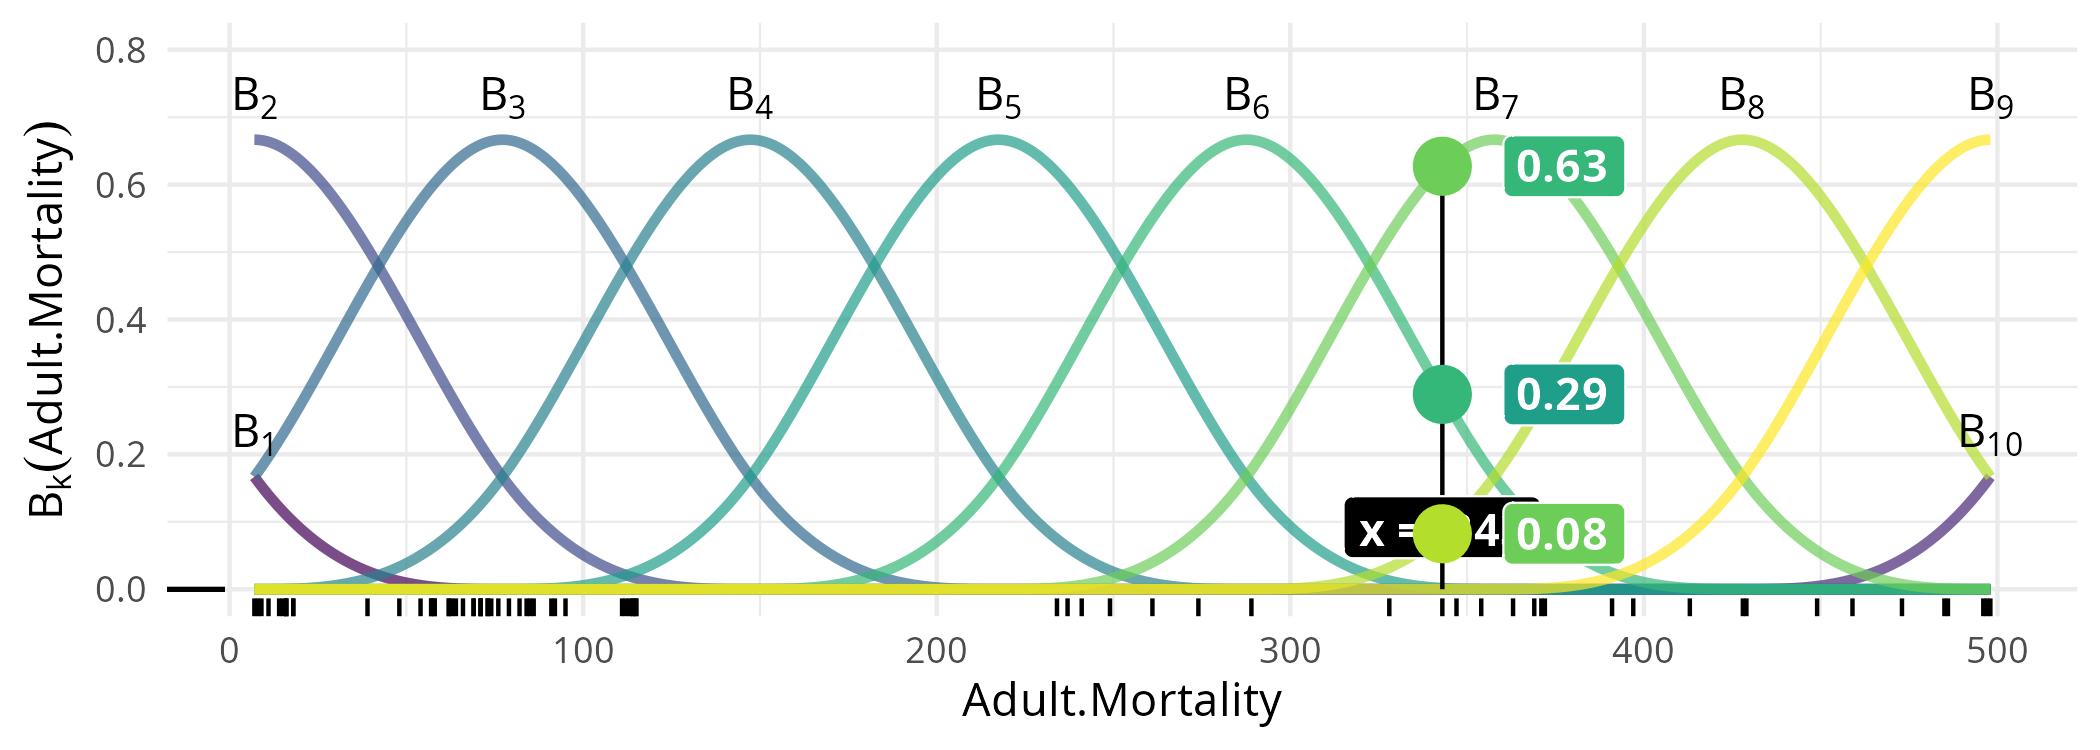
\includegraphics[width=0.7\textwidth]{figures/bs-base/fig-bs10.png}
    \end{figure}
  \end{center}
  \vspace{-0.3cm}
  \[
\design_k = \tiny\begin{blockarray}{cccccccccc}
\color[HTML]{440154}B_{1} & \color[HTML]{482878}B_{2} & \color[HTML]{3E4A89}B_{3} & \color[HTML]{31688E}B_{4} & \color[HTML]{26828E}B_{5} & \color[HTML]{1F9E89}B_{6} & \color[HTML]{35B779}B_{7} & \color[HTML]{6DCD59}B_{8} & \color[HTML]{B4DE2C}B_{9} & \color[HTML]{FDE725}B_{10} \\
\begin{block}{(cccccccccc)}
\phantom{x}\\
\color{lightgray}0.00 & \color{lightgray}0.00 & \color{lightgray}0.00 & \color{gray}0.07 & \color{gray}0.62 & \color{gray}0.31 & \color{lightgray}0.00 & \color{lightgray}0.00 & \color{lightgray}0.00 & \color{lightgray}0.00\color{black}\\
  \color{lightgray}0.00 & \color{gray}0.20 & \color{gray}0.66 & \color{gray}0.14 & \color{lightgray}0.00 & \color{lightgray}0.00 & \color{lightgray}0.00 & \color{lightgray}0.00 & \color{lightgray}0.00 & \color{lightgray}0.00\color{black}\\
  \color{lightgray}0.00 & \color{lightgray}0.00 & \color{lightgray}0.00 & \color{lightgray}0.00 & \color{lightgray}0.00 & \color{lightgray}0.00 & \color{lightgray}0.00 & \color{gray}0.17 & \color{gray}0.67 & \color{gray}0.17\color{black}\\
  \color{black}\vdots & \color{black}\vdots & \color{black}\vdots & \color{black}\vdots & \color{black}\vdots & \color{black}\vdots & \color{black}\vdots & \color{black}\vdots & \color{black}\vdots & \color{black}\vdots\\
  \color{lightgray}0.00 & \color{gray}0.02 & \color{gray}0.48 & \color{gray}0.48 & \color{gray}0.02 & \color{lightgray}0.00 & \color{lightgray}0.00 & \color{lightgray}0.00 & \color{lightgray}0.00 & \color{lightgray}0.00\color{black}\\
  \color{lightgray}0.00 & \color{lightgray}0.00 & \color{lightgray}0.00 & \color{gray}0.01 & \color{gray}0.40 & \color{gray}0.55 & \color{gray}0.04 & \color{lightgray}0.00 & \color{lightgray}0.00 & \color{lightgray}0.00\color{black}\\
  \color{lightgray}0.00 & \color{lightgray}0.00 & \color{lightgray}0.00 & \color{lightgray}0.00 & \color{lightgray}0.00 & \color[HTML]{1F9E89}0.29 & \color[HTML]{35B779}0.63 & \color[HTML]{6DCD59}0.08 & \color{lightgray}0.00 & \color{lightgray}0.00\color{black}\\
\phantom{x}\\
\end{block}
\end{blockarray}
\]
\normalsize

  \addtocounter{framenumber}{-1}
\end{frame}



\begin{frame}{Categorical base learner}
  \vspace{-0.3cm}\[g_k(x) = (g_{k,1}(x), \dots, g_{k,G}(x))^\tran = (\mathds{1}_{\{x = 1\}}, \dots, \mathds{1}_{\{x = G\}})^\tran, \ \ x\in\{1, \dots, G\}\]
  \begin{center}
    \begin{figure}
      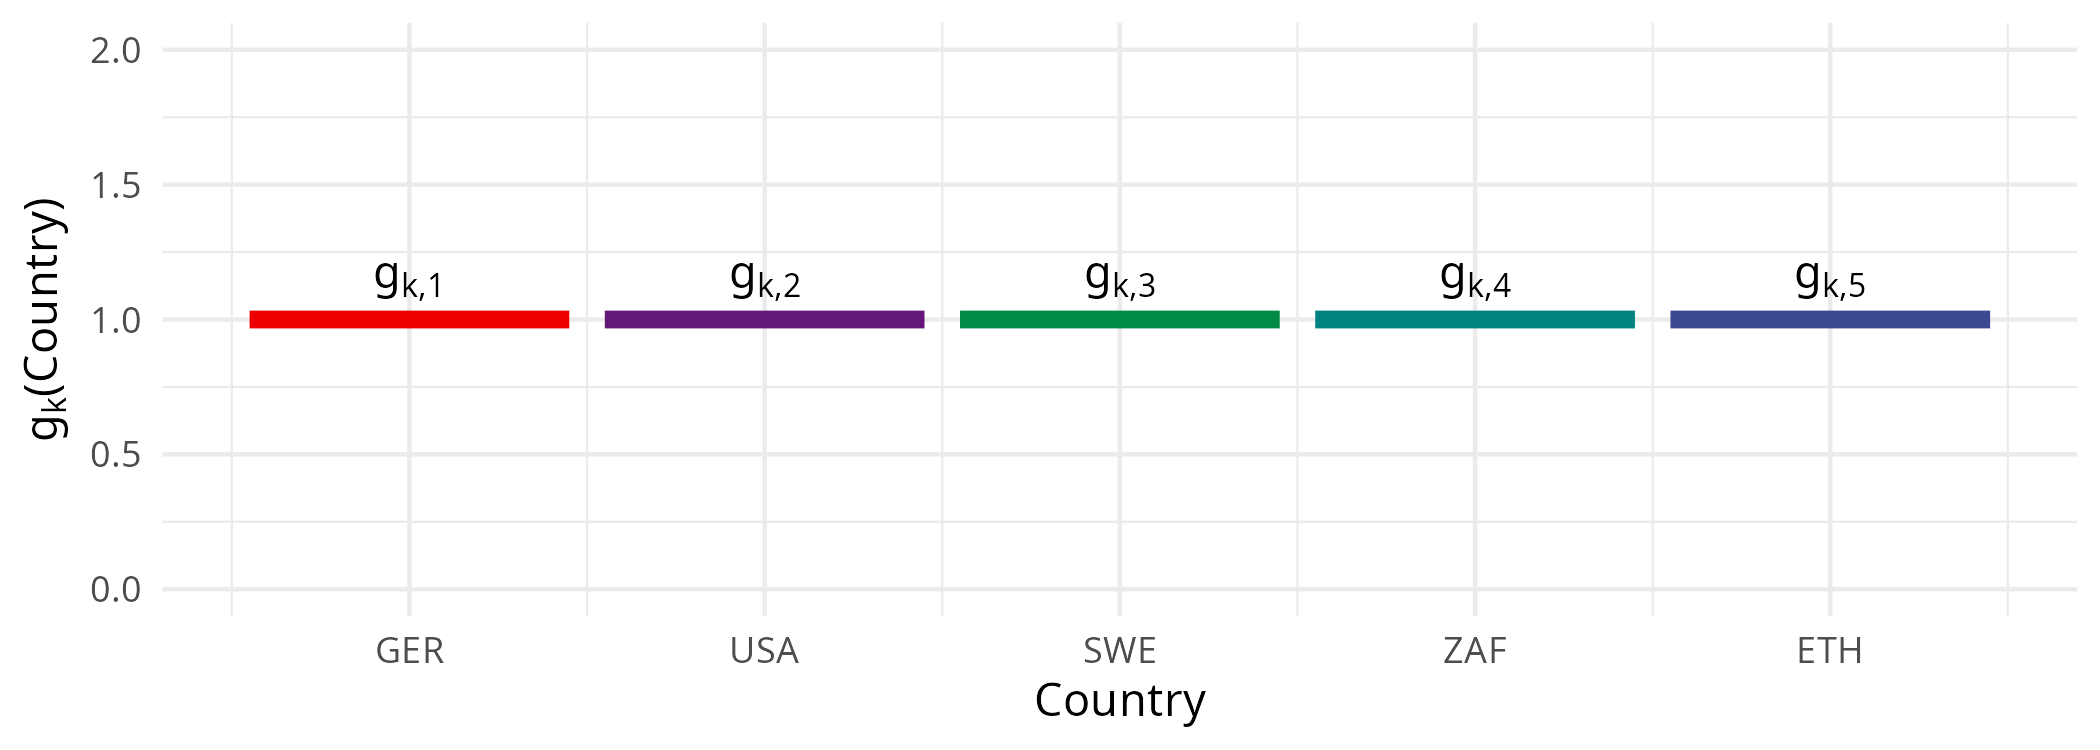
\includegraphics[width=0.7\textwidth]{figures/bs-cat/fig-cat0.png}
    \end{figure}
    \vspace{-0.5cm}
    \[
    \design_k = \left(\begin{array}{c}
      g_{k}^\tran(\xi[1]) \\
      \vdots \\
      g_{k}^\tran(\xi[n])
    \end{array}\right) = \left(\begin{array}{ccc}
      \mathds{1}_{\{\xi[1] = 1\}} & \dots & \mathds{1}_{\{\xi[1] = G\}} \\
      \vdots &  & \vdots \\
      \mathds{1}_{\{\xi[n] = 1\}} & \dots & \mathds{1}_{\{\xi[n] = G\}} \\
    \end{array}\right)\in\R^{n\times G}
    \]
  \end{center}

\end{frame}

\begin{frame}{Categorical base learner}
  \vspace{-0.3cm}\[g_k(x) = (g_{k,1}(x), \dots, g_{k,G}(x))^\tran = (\mathds{1}_{\{x = 1\}}, \dots, \mathds{1}_{\{x = G\}})^\tran, \ \ x\in\{1, \dots, G\}\]
  \begin{center}
    \begin{figure}
      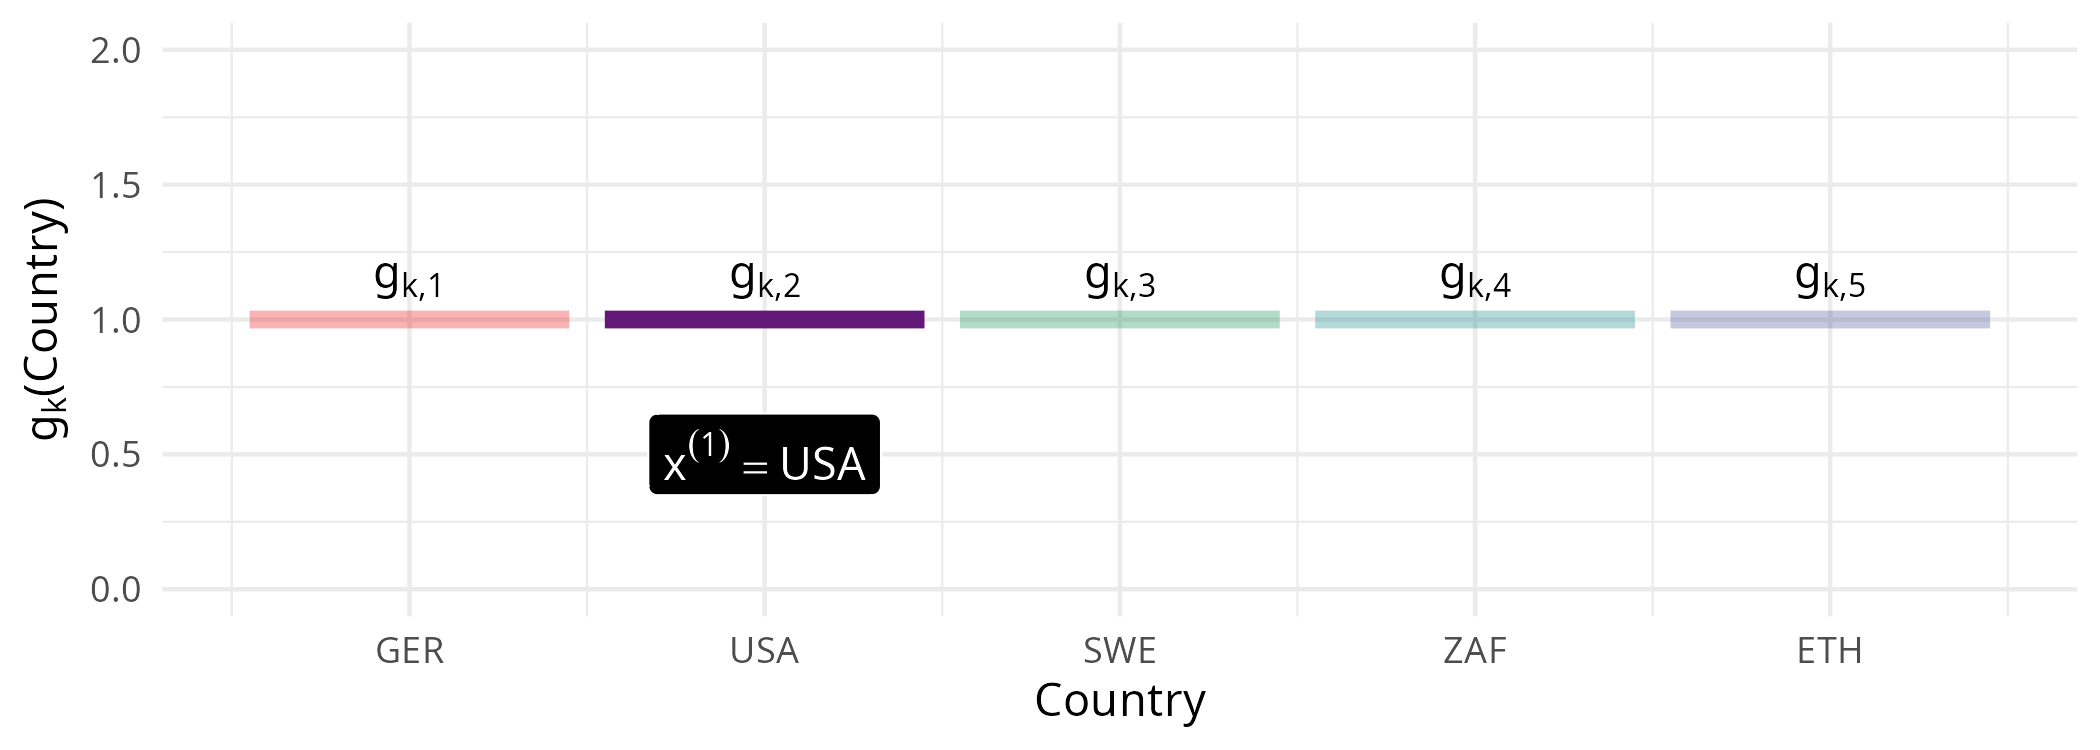
\includegraphics[width=0.7\textwidth]{figures/bs-cat/fig-cat1.png}
    \end{figure}
    \vspace{-0.5cm}
    \[
      \design_k = \tiny\begin{blockarray}{ccccc}
        \color[HTML]{EE0000}g_{k,GER} & \color[HTML]{631879}g_{k,USA} & \color[HTML]{008B45}g_{k,SWE} & \color[HTML]{008280}g_{k,ZAF} & \color[HTML]{3B4992}g_{k,ETH}\\
      \begin{block}{(ccccc)}
        \phantom{x}\\
        \color{lightgray}0 & \color[HTML]{631879}\bm{1} & \color{lightgray}0 & \color{lightgray}0 & \color{lightgray}0 \\
        \color{white}0 & \color{white}0 & \color{white}0 & \color{white}0 & \color{white}0 \\
        \color{white}0 & \color{white}0 & \color{white}0 & \color{white}0 & \color{white}0 \\
        \color{white}\vdots & \color{white}\vdots & \color{white}\vdots & \color{white}\vdots & \color{white}\vdots \\
        \color{white}0 & \color{white}0 & \color{white}0 & \color{white}0 & \color{white}0 \\
        \color{white}0 & \color{white}0 & \color{white}0 & \color{white}0 & \color{white}0 \\
        \color{white}0 & \color{white}0 & \color{white}0 & \color{white}0 & \color{white}0 \color{black}\\
        \phantom{x}
      \end{block}
    \end{blockarray}
    \]
    \normalsize
  \end{center}
\end{frame}

\begin{frame}{Categorical base learner}
  \vspace{-0.3cm}\[g_k(x) = (g_{k,1}(x), \dots, g_{k,G}(x))^\tran = (\mathds{1}_{\{x = 1\}}, \dots, \mathds{1}_{\{x = G\}})^\tran, \ \ x\in\{1, \dots, G\}\]
  \begin{center}
    \begin{figure}
      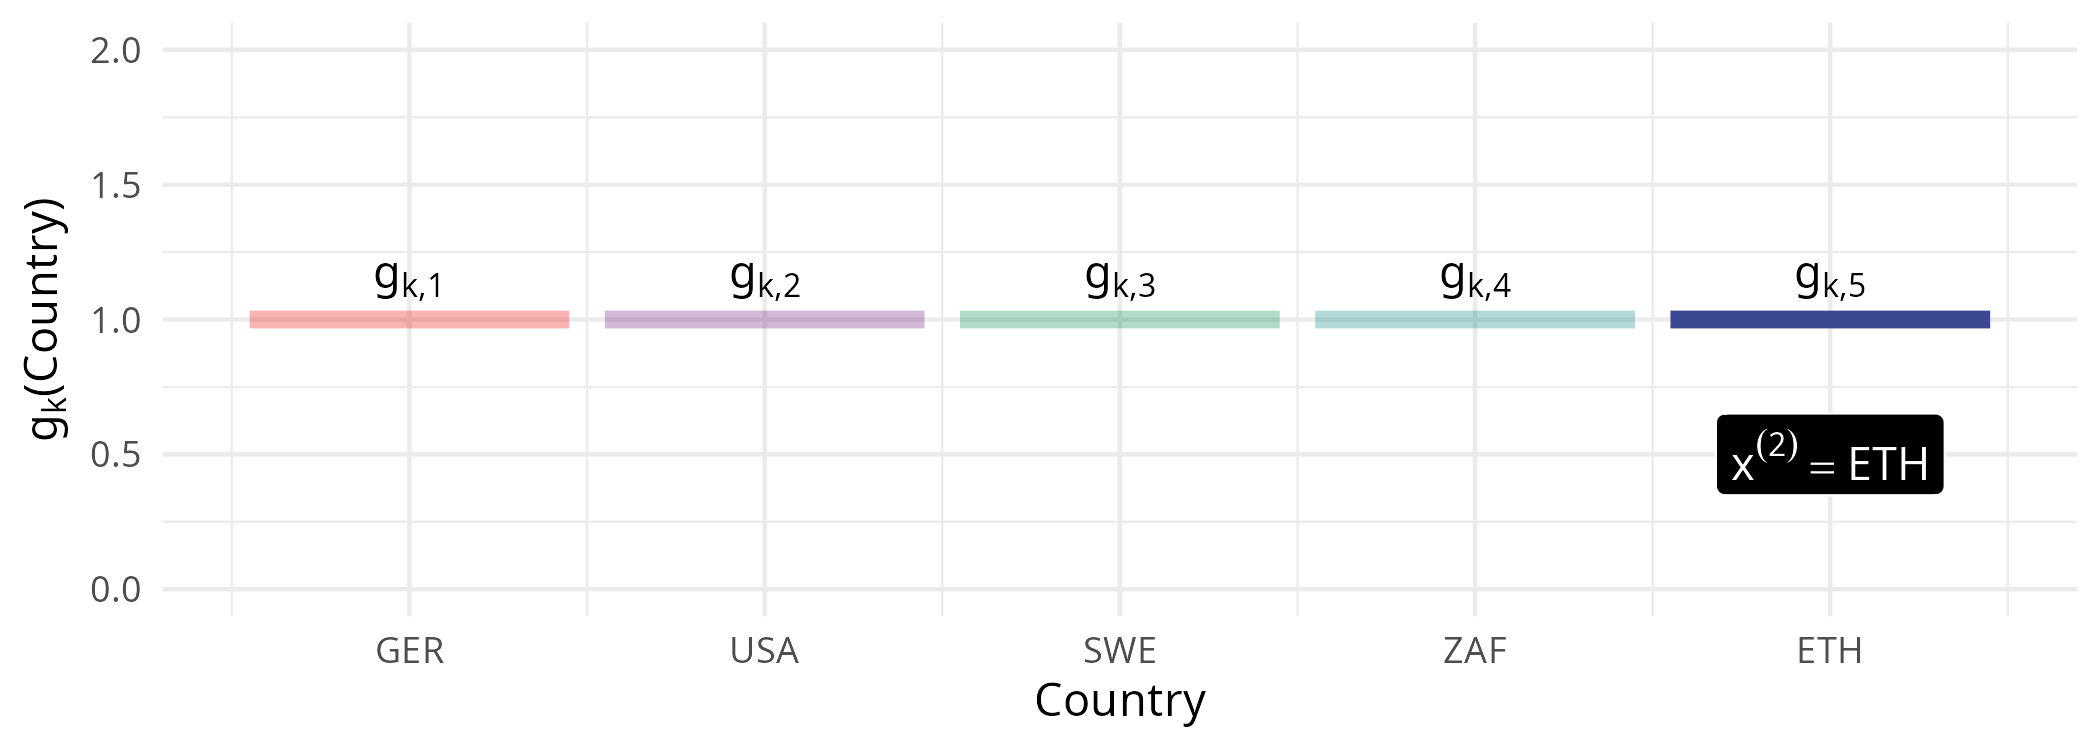
\includegraphics[width=0.7\textwidth]{figures/bs-cat/fig-cat2.png}
    \end{figure}
    \vspace{-0.5cm}
    \[
      \design_k = \tiny\begin{blockarray}{ccccc}
        \color[HTML]{EE0000}g_{k,GER} & \color[HTML]{631879}g_{k,USA} & \color[HTML]{008B45}g_{k,SWE} & \color[HTML]{008280}g_{k,ZAF} & \color[HTML]{3B4992}g_{k,ETH}\\
      \begin{block}{(ccccc)}
        \phantom{x}\\
        \color{lightgray}0 & \color{black}\bm{1} & \color{lightgray}0 & \color{lightgray}0 & \color{lightgray}0 \\
        \color{lightgray}0 & \color{lightgray}0 & \color{lightgray}0 & \color{lightgray}0 & \color[HTML]{3B4992}\bm{1} \\
        \color{white}0 & \color{white}0 & \color{white}0 & \color{white}0 & \color{white}0 \\
        \color{white}\vdots & \color{white}\vdots & \color{white}\vdots & \color{white}\vdots & \color{white}\vdots \\
        \color{white}0 & \color{white}0 & \color{white}0 & \color{white}0 & \color{white}0 \\
        \color{white}0 & \color{white}0 & \color{white}0 & \color{white}0 & \color{white}0 \\
        \color{white}0 & \color{white}0 & \color{white}0 & \color{white}0 & \color{white}0 \color{black}\\
        \phantom{x}\\
      \end{block}
    \end{blockarray}
    \]
    \normalsize
  \end{center}
  \addtocounter{framenumber}{-1}
\end{frame}

\begin{frame}{Categorical base learner}
  \vspace{-0.3cm}\[g_k(x) = (g_{k,1}(x), \dots, g_{k,G}(x))^\tran = (\mathds{1}_{\{x = 1\}}, \dots, \mathds{1}_{\{x = G\}})^\tran, \ \ x\in\{1, \dots, G\}\]
  \begin{center}
    \begin{figure}
      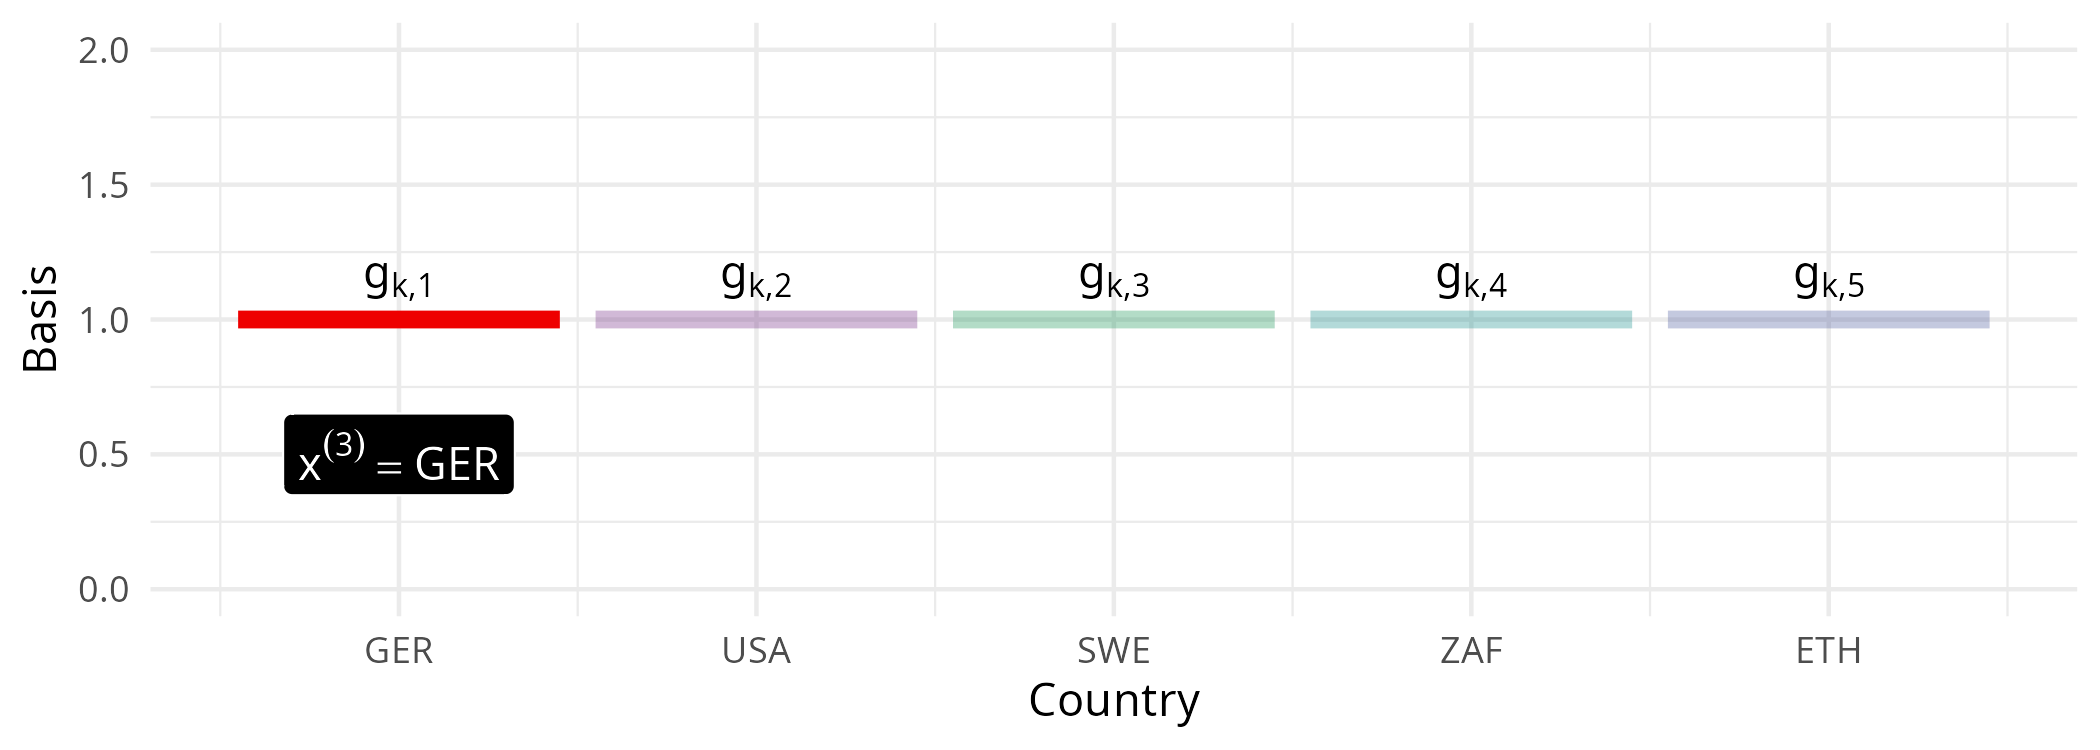
\includegraphics[width=0.7\textwidth]{figures/bs-cat/fig-cat3.png}
    \end{figure}
    \vspace{-0.5cm}
    \[
      \design_k = \tiny\begin{blockarray}{ccccc}
        \color[HTML]{EE0000}g_{k,GER} & \color[HTML]{631879}g_{k,USA} & \color[HTML]{008B45}g_{k,SWE} & \color[HTML]{008280}g_{k,ZAF} & \color[HTML]{3B4992}g_{k,ETH}\\
      \begin{block}{(ccccc)}
        \phantom{x}\\
        \color{lightgray}0 & \color{black}\bm{1} & \color{lightgray}0 & \color{lightgray}0 & \color{lightgray}0 \\
        \color{lightgray}0 & \color{lightgray}0 & \color{lightgray}0 & \color{lightgray}0 & \color{black}\bm{1} \\
        \color[HTML]{EE0000}\bm{1} & \color{lightgray}0 & \color{lightgray}0 & \color{lightgray}0 & \color{lightgray}0 \\
        \color{white}\vdots & \color{white}\vdots & \color{white}\vdots & \color{white}\vdots & \color{white}\vdots \\
        \color{white}0 & \color{white}0 & \color{white}0 & \color{white}0 & \color{white}0 \\
        \color{white}0 & \color{white}0 & \color{white}0 & \color{white}0 & \color{white}0 \\
        \color{white}0 & \color{white}0 & \color{white}0 & \color{white}0 & \color{white}0 \color{black}\\
        \phantom{x}\\
      \end{block}
    \end{blockarray}
    \]
    \normalsize
  \end{center}
  \addtocounter{framenumber}{-1}
\end{frame}

\begin{frame}{Categorical base learner}
  \vspace{-0.3cm}\[g_k(x) = (g_{k,1}(x), \dots, g_{k,G}(x))^\tran = (\mathds{1}_{\{x = 1\}}, \dots, \mathds{1}_{\{x = G\}})^\tran, \ \ x\in\{1, \dots, G\}\]
  \begin{center}
    \begin{figure}
      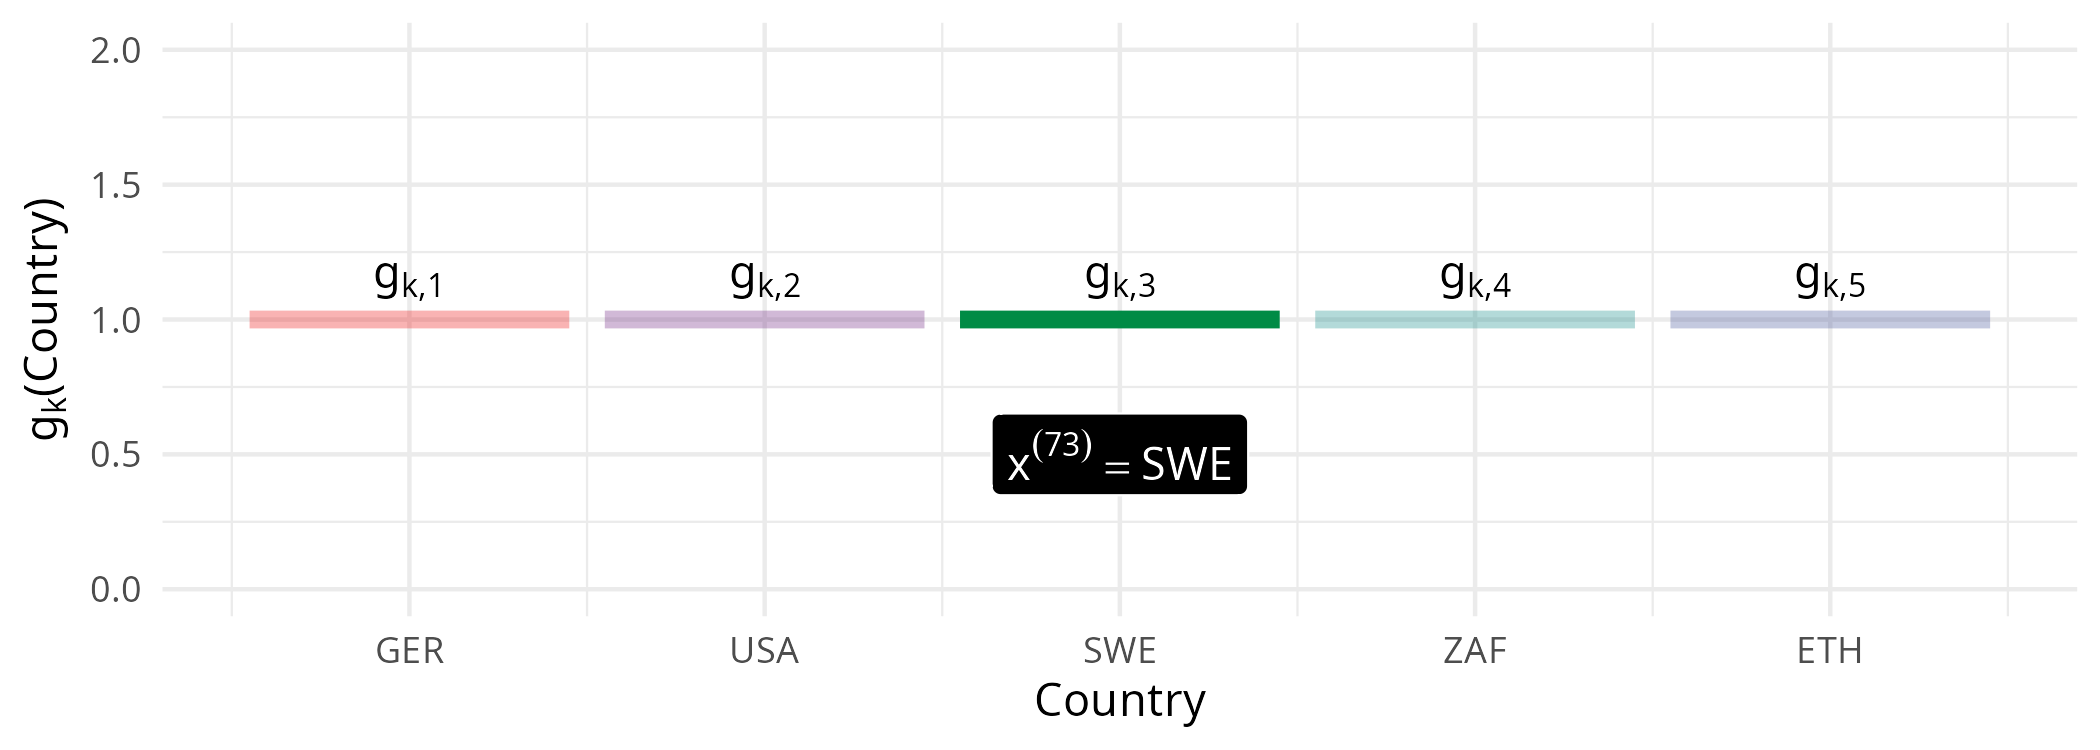
\includegraphics[width=0.7\textwidth]{figures/bs-cat/fig-cat4.png}
    \end{figure}
    \vspace{-0.5cm}
    \[
      \design_k = \tiny\begin{blockarray}{ccccc}
        \color[HTML]{EE0000}g_{k,GER} & \color[HTML]{631879}g_{k,USA} & \color[HTML]{008B45}g_{k,SWE} & \color[HTML]{008280}g_{k,ZAF} & \color[HTML]{3B4992}g_{k,ETH}\\
      \begin{block}{(ccccc)}
        \phantom{x}\\
        \color{lightgray}0 & \color{black}\bm{1} & \color{lightgray}0 & \color{lightgray}0 & \color{lightgray}0 \\
        \color{lightgray}0 & \color{lightgray}0 & \color{lightgray}0 & \color{lightgray}0 & \color{black}\bm{1} \\
        \color{black}\bm{1} & \color{lightgray}0 & \color{lightgray}0 & \color{lightgray}0 & \color{lightgray}0 \\
        \color{lightgray}\vdots & \color{lightgray}\vdots & \color{lightgray}\vdots & \color{lightgray}\vdots & \color{lightgray}\vdots \\
        \color{lightgray}0 & \color{lightgray}0 & \color[HTML]{008B45}\bm{1} & \color{lightgray}0 & \color{lightgray}0 \\
        \color{white}0 & \color{white}0 & \color{white}0 & \color{white}0 & \color{white}0 \\
        \color{white}0 & \color{white}0 & \color{white}0 & \color{white}0 & \color{white}0 \color{black}\\
        \phantom{x}\\
      \end{block}
    \end{blockarray}
    \]
    \normalsize
  \end{center}
  \addtocounter{framenumber}{-1}
\end{frame}

\begin{frame}{Categorical base learner}
  \vspace{-0.3cm}\[g_k(x) = (g_{k,1}(x), \dots, g_{k,G}(x))^\tran = (\mathds{1}_{\{x = 1\}}, \dots, \mathds{1}_{\{x = G\}})^\tran, \ \ x\in\{1, \dots, G\}\]
  \begin{center}
    \begin{figure}
      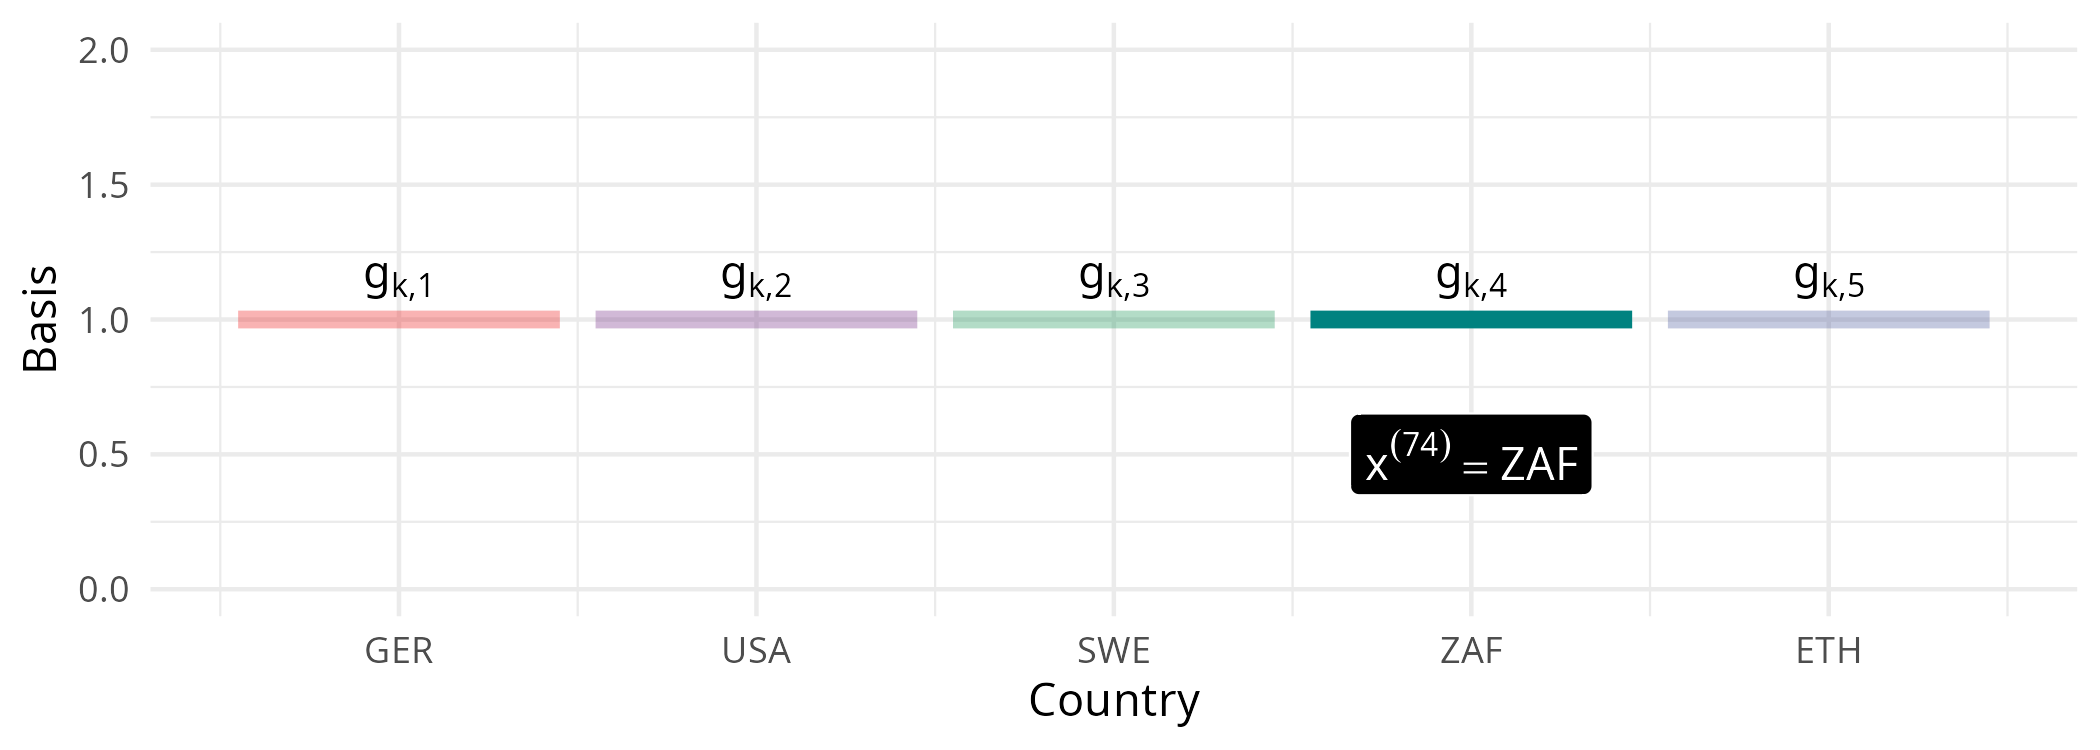
\includegraphics[width=0.7\textwidth]{figures/bs-cat/fig-cat5.png}
    \end{figure}
    \vspace{-0.5cm}
    \[
      \design_k = \tiny\begin{blockarray}{ccccc}
        \color[HTML]{EE0000}g_{k,GER} & \color[HTML]{631879}g_{k,USA} & \color[HTML]{008B45}g_{k,SWE} & \color[HTML]{008280}g_{k,ZAF} & \color[HTML]{3B4992}g_{k,ETH}\\
      \begin{block}{(ccccc)}
        \phantom{x}\\
        \color{lightgray}0 & \color{black}\bm{1} & \color{lightgray}0 & \color{lightgray}0 & \color{lightgray}0 \\
        \color{lightgray}0 & \color{lightgray}0 & \color{lightgray}0 & \color{lightgray}0 & \color{black}\bm{1} \\
        \color{black}\bm{1} & \color{lightgray}0 & \color{lightgray}0 & \color{lightgray}0 & \color{lightgray}0 \\
        \color{lightgray}\vdots & \color{lightgray}\vdots & \color{lightgray}\vdots & \color{lightgray}\vdots & \color{lightgray}\vdots \\
        \color{lightgray}0 & \color{lightgray}0 & \color{black}\bm{1} & \color{lightgray}0 & \color{lightgray}0 \\
        \color{lightgray}0 & \color{lightgray}0 & \color{lightgray}0 & \color[HTML]{008280}\bm{1} & \color{lightgray}0 \\
        \color{white}0 & \color{white}0 & \color{white}0 & \color{white}0 & \color{white}0 \color{black}\\
        \phantom{x}\\
      \end{block}
    \end{blockarray}
    \]
    \normalsize
  \end{center}
  \addtocounter{framenumber}{-1}
\end{frame}

\begin{frame}{Categorical base learner}
  \vspace{-0.3cm}\[g_k(x) = (g_{k,1}(x), \dots, g_{k,G}(x))^\tran = (\mathds{1}_{\{x = 1\}}, \dots, \mathds{1}_{\{x = G\}})^\tran, \ \ x\in\{1, \dots, G\}\]
  \begin{center}
    \begin{figure}
      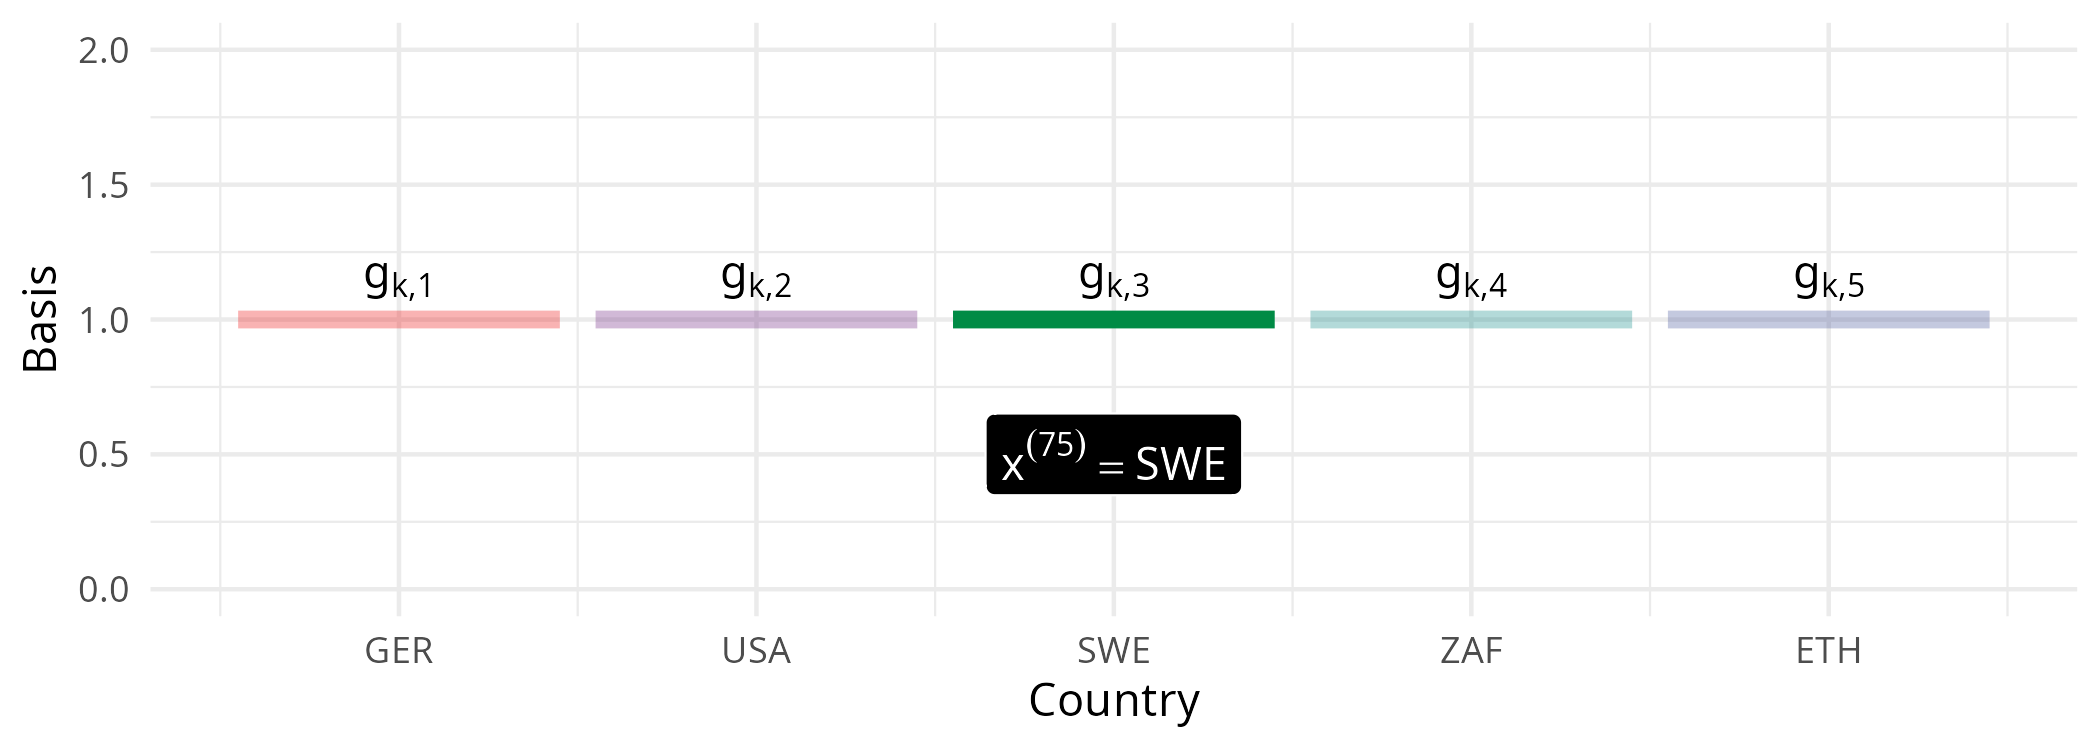
\includegraphics[width=0.7\textwidth]{figures/bs-cat/fig-cat6.png}
    \end{figure}
    \vspace{-0.5cm}
    \[
      \design_k = \tiny\begin{blockarray}{ccccc}
        \color[HTML]{EE0000}g_{k,GER} & \color[HTML]{631879}g_{k,USA} & \color[HTML]{008B45}g_{k,SWE} & \color[HTML]{008280}g_{k,ZAF} & \color[HTML]{3B4992}g_{k,ETH}\\
      \begin{block}{(ccccc)}
        \phantom{x}\\
        \color{lightgray}0 & \color{black}\bm{1} & \color{lightgray}0 & \color{lightgray}0 & \color{lightgray}0 \\
        \color{lightgray}0 & \color{lightgray}0 & \color{lightgray}0 & \color{lightgray}0 & \color{black}\bm{1} \\
        \color{black}\bm{1} & \color{lightgray}0 & \color{lightgray}0 & \color{lightgray}0 & \color{lightgray}0 \\
        \color{lightgray}\vdots & \color{lightgray}\vdots & \color{lightgray}\vdots & \color{lightgray}\vdots & \color{lightgray}\vdots \\
        \color{lightgray}0 & \color{lightgray}0 & \color{black}\bm{1} & \color{lightgray}0 & \color{lightgray}0 \\
        \color{lightgray}0 & \color{lightgray}0 & \color{lightgray}0 & \color{black}\bm{1} & \color{lightgray}0 \\
        \color{lightgray}0 & \color{lightgray}0 & \color[HTML]{008B45}\bm{1} & \color{lightgray}0 & \color{lightgray}0 \\
        \phantom{x}\\
      \end{block}
    \end{blockarray}
    \]
    \normalsize
  \end{center}
  \addtocounter{framenumber}{-1}
\end{frame}






\begin{frame}{(Row-wise) tensor product (RWTP) base learner}
  Combination (interaction) $b_k \odot b_l$ between to base learners $b_k$ and $b_l$:
  \[g_k(\xv) \otimes g_l(\xv) = (g_{k,1}(\xv)g_l(\xv)^\tran, \dots, g_{k,d_k}(\xv)g_l(\xv)^\tran)^\tran \]
  Design matrix:
  \[
  \design_k \odot \design_l = \left(\begin{array}{c}
    (g_{k}(\xi[1]) \otimes g_l(\xi[1]))^\tran \\
    \vdots \\
    (g_{k}(\xi[n]) \otimes g_l(\xi[n]))^\tran
  \end{array}\right) \in\R^{n\times d_k d_l}
  \]
\end{frame}





\begin{frame}{(Row-wise) tensor product (RWTP) base learner}
  Example:
  \begin{itemize}
    \item $b_k$ encodes the country: $g_k(x) = (\mathds{1}_{\{x = 1\}}, \dots, \mathds{1}_{\{x = G\}})^\tran$
    \item $b_l$ uses a B-spline basis for BMI: $g_l(x) = (B_{k,1}(x), \dots, B_{k,d_k}(x))^\tran$
  \end{itemize}
  $$
    \design_k \odot \design_l = \tiny\begin{blockarray}{ccccc}
      \color[HTML]{EE0000}g_{k,GER} & \color[HTML]{631879}g_{k,USA} & \color[HTML]{008B45}g_{k,SWE} & \color[HTML]{008280}g_{k,ZAF} & \color[HTML]{3B4992}g_{k,ETH}\\
    \begin{block}{(ccccc)}
      \phantom{x}\\
      \color{lightgray}0 & \color[HTML]{631879}\bm{g_l(x^{(1)})} & \color{lightgray}0 & \color{lightgray}0 & \color{lightgray}0 \\
      \color{white}0 & \color{white}0 & \color{white}0 & \color{white}0 & \color{white}\bm{g_l(x^{(2)})} \\
      \color{white}\bm{g_l(x^{(3)})} & \color{white}0 & \color{white}0 & \color{white}0 & \color{white}0 \\
      \color{white}\vdots & \color{white}\vdots & \color{white}\vdots & \color{white}\vdots & \color{white}\vdots \\
      \color{white}0 & \color{white}0 & \color{white}\bm{g_l(x^{(73)})} & \color{white}0 & \color{white}0 \\
      \color{white}0 & \color{white}0 & \color{white}0 & \color{white}\bm{g_l(x^{(74)})} & \color{white}0 \\
      \color{white}0 & \color{white}0 & \color{white}\bm{g_l(x^{(75)})} & \color{white}0 & \color{white}0 \\
      \phantom{x}\\
    \end{block}
  \end{blockarray}
  $$
  \normalsize
  {\transparent{0.2}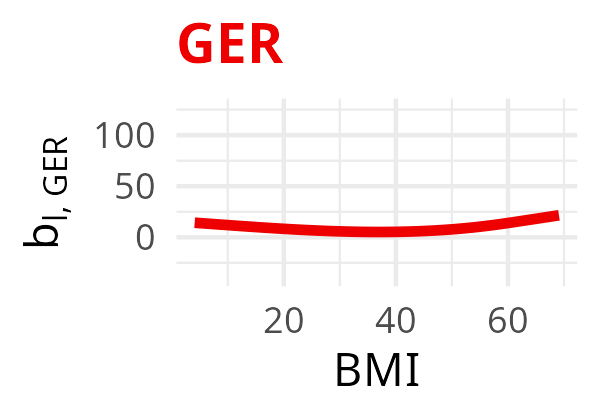
\includegraphics[width=0.19\textwidth]{figures/bs-tensor/fig-tensor-GER.png}}
  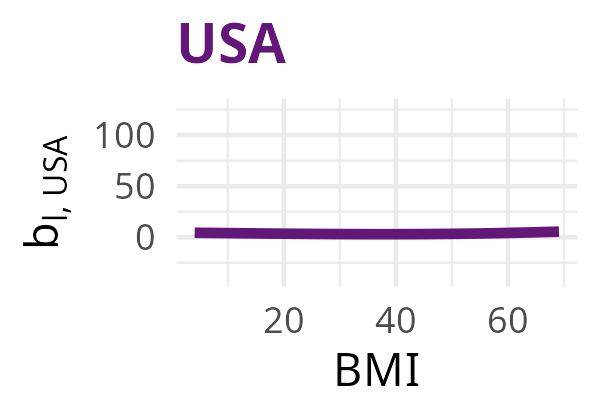
\includegraphics[width=0.19\textwidth]{figures/bs-tensor/fig-tensor-USA.png}
  {\transparent{0.2}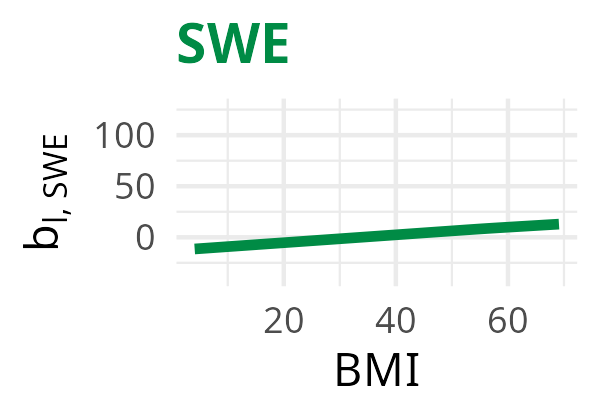
\includegraphics[width=0.19\textwidth]{figures/bs-tensor/fig-tensor-SWE.png}}
  {\transparent{0.2}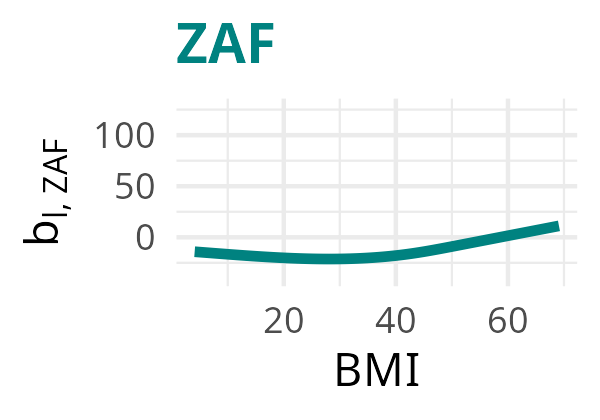
\includegraphics[width=0.19\textwidth]{figures/bs-tensor/fig-tensor-ZAF.png}}
  {\transparent{0.2}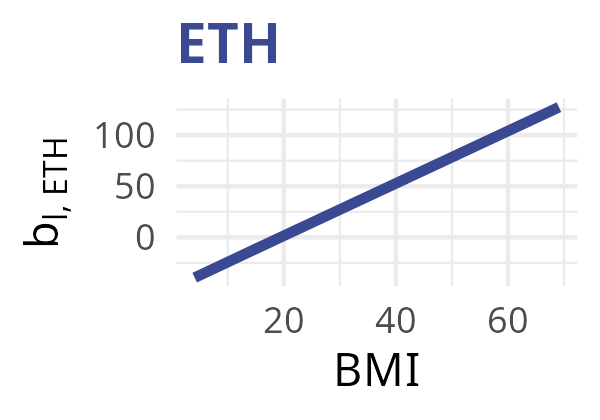
\includegraphics[width=0.19\textwidth]{figures/bs-tensor/fig-tensor-ETH.png}}
\end{frame}

\begin{frame}{(Row-wise) tensor product (RWTP) base learner}
  Example:
  \begin{itemize}
    \item $b_k$ encodes the country: $g_k(x) = (\mathds{1}_{\{x = 1\}}, \dots, \mathds{1}_{\{x = G\}})^\tran$
    \item $b_l$ uses a B-spline basis for BMI: $g_l(x) = (B_{k,1}(x), \dots, B_{k,d_k}(x))^\tran$
  \end{itemize}
  $$
    \design_k \odot \design_l = \tiny\begin{blockarray}{ccccc}
      \color[HTML]{EE0000}g_{k,GER} & \color[HTML]{631879}g_{k,USA} & \color[HTML]{008B45}g_{k,SWE} & \color[HTML]{008280}g_{k,ZAF} & \color[HTML]{3B4992}g_{k,ETH}\\
    \begin{block}{(ccccc)}
      \phantom{x}\\
      \color{lightgray}0 & \color{black}\bm{g_l(x^{(1)})} & \color{lightgray}0 & \color{lightgray}0 & \color{lightgray}0 \\
      \color{lightgray}0 & \color{lightgray}0 & \color{lightgray}0 & \color{lightgray}0 & \color[HTML]{3B4992}\bm{g_l(x^{(2)})} \\
      \color{white}\bm{g_l(x^{(3)})} & \color{white}0 & \color{white}0 & \color{white}0 & \color{white}0 \\
      \color{white}\vdots & \color{white}\vdots & \color{white}\vdots & \color{white}\vdots & \color{white}\vdots \\
      \color{white}0 & \color{white}0 & \color{white}\bm{g_l(x^{(73)})} & \color{white}0 & \color{white}0 \\
      \color{white}0 & \color{white}0 & \color{white}0 & \color{white}\bm{g_l(x^{(74)})} & \color{white}0 \\
      \color{white}0 & \color{white}0 & \color{white}\bm{g_l(x^{(75)})} & \color{white}0 & \color{white}0 \\
      \phantom{x}\\
    \end{block}
  \end{blockarray}
  $$
  \normalsize
  {\transparent{0.2}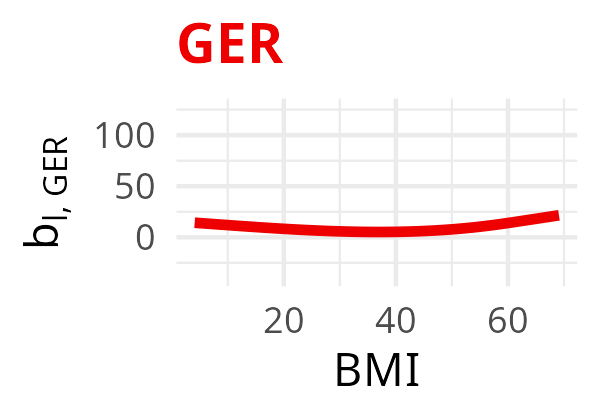
\includegraphics[width=0.19\textwidth]{figures/bs-tensor/fig-tensor-GER.png}}
  {\transparent{0.2}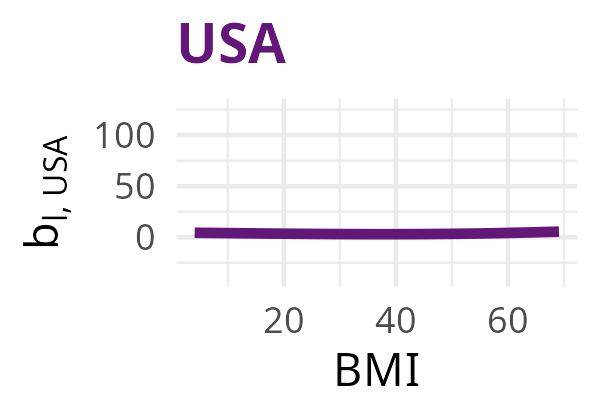
\includegraphics[width=0.19\textwidth]{figures/bs-tensor/fig-tensor-USA.png}}
  {\transparent{0.2}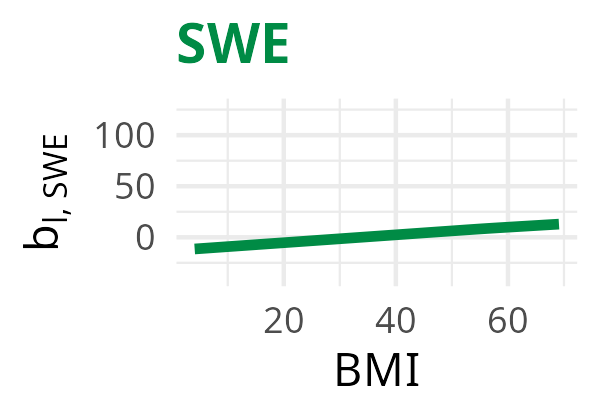
\includegraphics[width=0.19\textwidth]{figures/bs-tensor/fig-tensor-SWE.png}}
  {\transparent{0.2}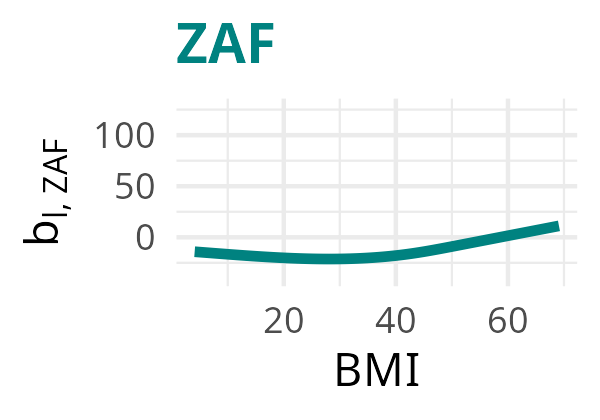
\includegraphics[width=0.19\textwidth]{figures/bs-tensor/fig-tensor-ZAF.png}}
  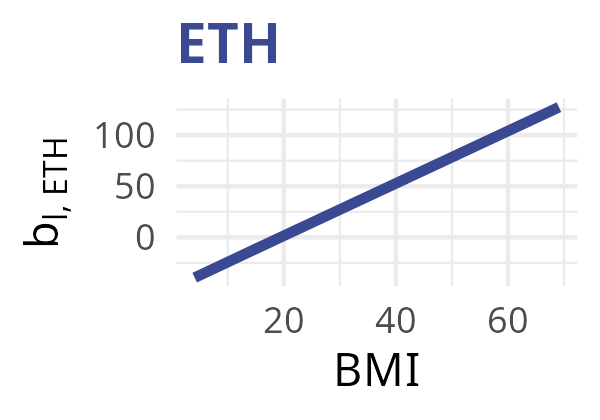
\includegraphics[width=0.19\textwidth]{figures/bs-tensor/fig-tensor-ETH.png}
  \addtocounter{framenumber}{-1}
\end{frame}

\begin{frame}{(Row-wise) tensor product (RWTP) base learner}
  Example:
  \begin{itemize}
    \item $b_k$ encodes the country: $g_k(x) = (\mathds{1}_{\{x = 1\}}, \dots, \mathds{1}_{\{x = G\}})^\tran$
    \item $b_l$ uses a B-spline basis for BMI: $g_l(x) = (B_{k,1}(x), \dots, B_{k,d_k}(x))^\tran$
  \end{itemize}
  $$
    \design_k \odot \design_l = \tiny\begin{blockarray}{ccccc}
      \color[HTML]{EE0000}g_{k,GER} & \color[HTML]{631879}g_{k,USA} & \color[HTML]{008B45}g_{k,SWE} & \color[HTML]{008280}g_{k,ZAF} & \color[HTML]{3B4992}g_{k,ETH}\\
    \begin{block}{(ccccc)}
      \phantom{x}\\
      \color{lightgray}0 & \color{black}\bm{g_l(x^{(1)})} & \color{lightgray}0 & \color{lightgray}0 & \color{lightgray}0 \\
      \color{lightgray}0 & \color{lightgray}0 & \color{lightgray}0 & \color{lightgray}0 & \color{black}\bm{g_l(x^{(2)})} \\
      \color[HTML]{EE0000}\bm{g_l(x^{(3)})} & \color{lightgray}0 & \color{lightgray}0 & \color{lightgray}0 & \color{lightgray}0 \\
      \color{white}\vdots & \color{white}\vdots & \color{white}\vdots & \color{white}\vdots & \color{white}\vdots \\
      \color{white}0 & \color{white}0 & \color{white}\bm{g_l(x^{(73)})} & \color{white}0 & \color{white}0 \\
      \color{white}0 & \color{white}0 & \color{white}0 & \color{white}\bm{g_l(x^{(74)})} & \color{white}0 \\
      \color{white}0 & \color{white}0 & \color{white}\bm{g_l(x^{(75)})} & \color{white}0 & \color{white}0 \\
      \phantom{x}\\
    \end{block}
  \end{blockarray}
  $$
  \normalsize
  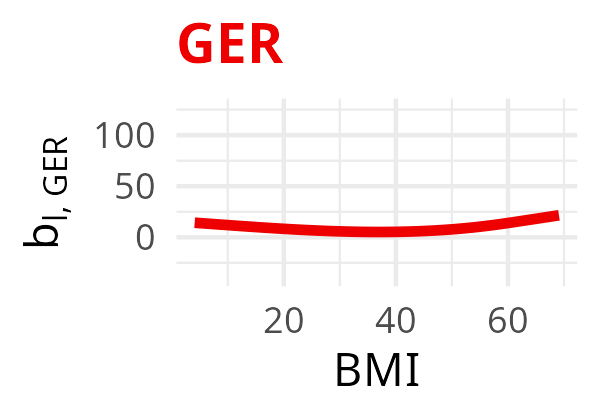
\includegraphics[width=0.19\textwidth]{figures/bs-tensor/fig-tensor-GER.png}
  {\transparent{0.2}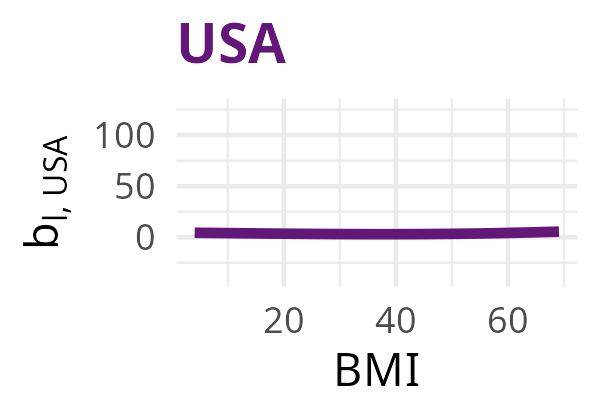
\includegraphics[width=0.19\textwidth]{figures/bs-tensor/fig-tensor-USA.png}}
  {\transparent{0.2}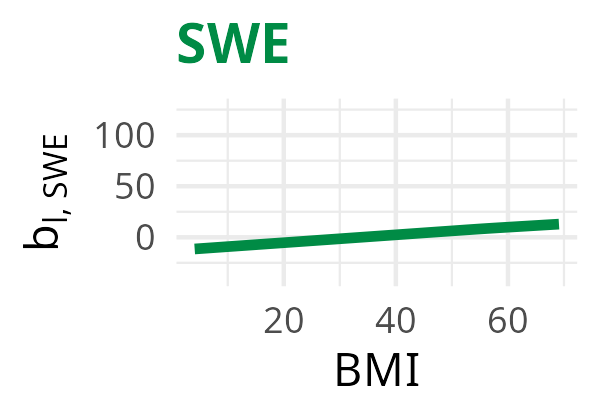
\includegraphics[width=0.19\textwidth]{figures/bs-tensor/fig-tensor-SWE.png}}
  {\transparent{0.2}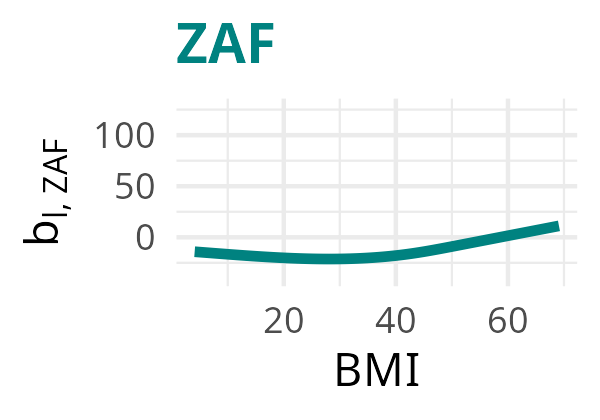
\includegraphics[width=0.19\textwidth]{figures/bs-tensor/fig-tensor-ZAF.png}}
  {\transparent{0.2}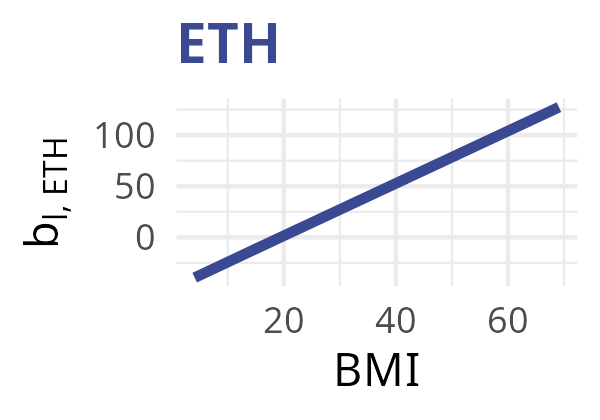
\includegraphics[width=0.19\textwidth]{figures/bs-tensor/fig-tensor-ETH.png}}
  \addtocounter{framenumber}{-1}
\end{frame}

\begin{frame}{(Row-wise) tensor product (RWTP) base learner}
  Example:
  \begin{itemize}
    \item $b_k$ encodes the country: $g_k(x) = (\mathds{1}_{\{x = 1\}}, \dots, \mathds{1}_{\{x = G\}})^\tran$
    \item $b_l$ uses a B-spline basis for BMI: $g_l(x) = (B_{k,1}(x), \dots, B_{k,d_k}(x))^\tran$
  \end{itemize}
  $$
    \design_k \odot \design_l = \tiny\begin{blockarray}{ccccc}
      \color[HTML]{EE0000}g_{k,GER} & \color[HTML]{631879}g_{k,USA} & \color[HTML]{008B45}g_{k,SWE} & \color[HTML]{008280}g_{k,ZAF} & \color[HTML]{3B4992}g_{k,ETH}\\
    \begin{block}{(ccccc)}
      \phantom{x}\\
      \color{lightgray}0 & \color{black}\bm{g_l(x^{(1)})} & \color{lightgray}0 & \color{lightgray}0 & \color{lightgray}0 \\
      \color{lightgray}0 & \color{lightgray}0 & \color{lightgray}0 & \color{lightgray}0 & \color{black}\bm{g_l(x^{(2)})} \\
      \color{black}\bm{g_l(x^{(3)})} & \color{lightgray}0 & \color{lightgray}0 & \color{lightgray}0 & \color{lightgray}0 \\
      \color{lightgray}\vdots & \color{lightgray}\vdots & \color{lightgray}\vdots & \color{lightgray}\vdots & \color{lightgray}\vdots \\
      \color{lightgray}0 & \color{lightgray}0 & \color[HTML]{008B45}\bm{g_l(x^{(73)})} & \color{lightgray}0 & \color{lightgray}0 \\
      \color{white}0 & \color{white}0 & \color{white}0 & \color{white}\bm{g_l(x^{(74)})} & \color{white}0 \\
      \color{white}0 & \color{white}0 & \color{white}\bm{g_l(x^{(75)})} & \color{white}0 & \color{white}0 \\
      \phantom{x}\\
    \end{block}
  \end{blockarray}
  $$
  \normalsize
  {\transparent{0.2}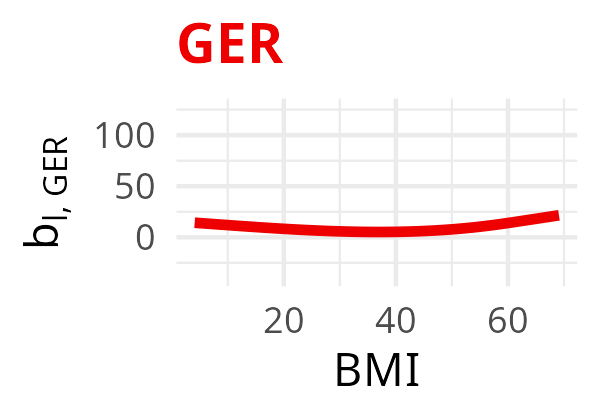
\includegraphics[width=0.19\textwidth]{figures/bs-tensor/fig-tensor-GER.png}}
  {\transparent{0.2}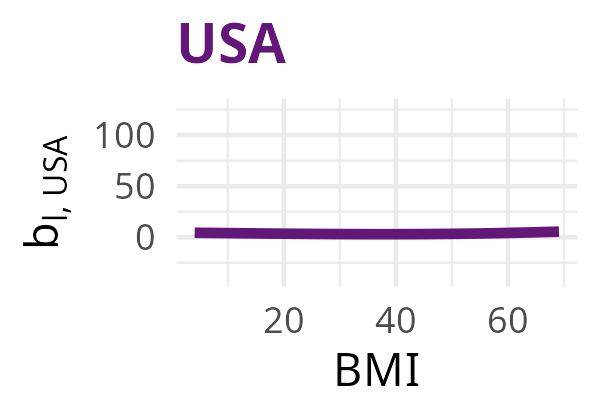
\includegraphics[width=0.19\textwidth]{figures/bs-tensor/fig-tensor-USA.png}}
  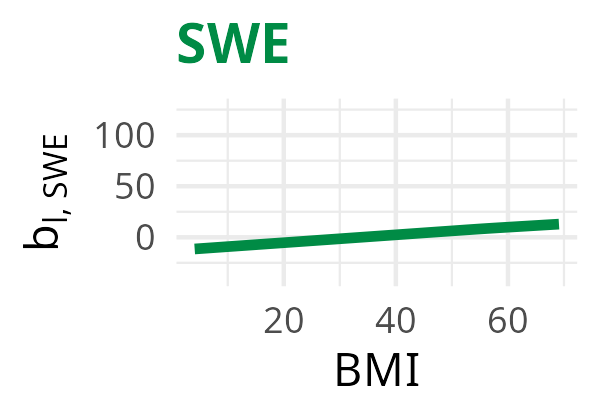
\includegraphics[width=0.19\textwidth]{figures/bs-tensor/fig-tensor-SWE.png}
  {\transparent{0.2}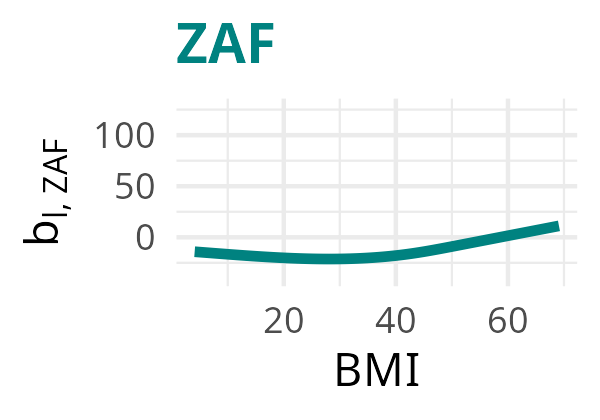
\includegraphics[width=0.19\textwidth]{figures/bs-tensor/fig-tensor-ZAF.png}}
  {\transparent{0.2}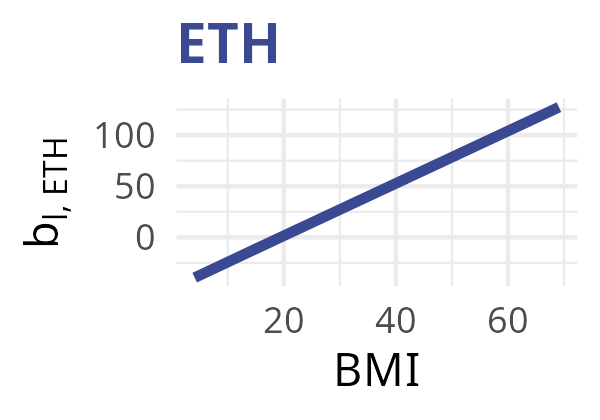
\includegraphics[width=0.19\textwidth]{figures/bs-tensor/fig-tensor-ETH.png}}
  \addtocounter{framenumber}{-1}
\end{frame}

\begin{frame}{(Row-wise) tensor product (RWTP) base learner}
  Example:
  \begin{itemize}
    \item $b_k$ encodes the country: $g_k(x) = (\mathds{1}_{\{x = 1\}}, \dots, \mathds{1}_{\{x = G\}})^\tran$
    \item $b_l$ uses a B-spline basis for BMI: $g_l(x) = (B_{k,1}(x), \dots, B_{k,d_k}(x))^\tran$
  \end{itemize}
  $$
    \design_k \odot \design_l = \tiny\begin{blockarray}{ccccc}
      \color[HTML]{EE0000}g_{k,GER} & \color[HTML]{631879}g_{k,USA} & \color[HTML]{008B45}g_{k,SWE} & \color[HTML]{008280}g_{k,ZAF} & \color[HTML]{3B4992}g_{k,ETH}\\
    \begin{block}{(ccccc)}
      \phantom{x}\\
      \color{lightgray}0 & \color{black}\bm{g_l(x^{(1)})} & \color{lightgray}0 & \color{lightgray}0 & \color{lightgray}0 \\
      \color{lightgray}0 & \color{lightgray}0 & \color{lightgray}0 & \color{lightgray}0 & \color{black}\bm{g_l(x^{(2)})} \\
      \color{black}\bm{g_l(x^{(3)})} & \color{lightgray}0 & \color{lightgray}0 & \color{lightgray}0 & \color{lightgray}0 \\
      \color{lightgray}\vdots & \color{lightgray}\vdots & \color{lightgray}\vdots & \color{lightgray}\vdots & \color{lightgray}\vdots \\
      \color{lightgray}0 & \color{lightgray}0 & \color{black}\bm{g_l(x^{(73)})} & \color{lightgray}0 & \color{lightgray}0 \\
      \color{lightgray}0 & \color{lightgray}0 & \color{lightgray}0 & \color[HTML]{008280}\bm{g_l(x^{(74)})} & \color{lightgray}0 \\
      \color{white}0 & \color{white}0 & \color{white}\bm{g_l(x^{(75)})} & \color{white}0 & \color{white}0 \\
      \phantom{x}\\
    \end{block}
  \end{blockarray}
  $$
  \normalsize
  {\transparent{0.2}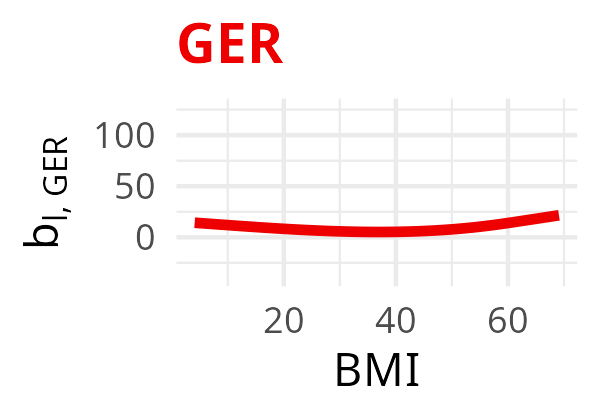
\includegraphics[width=0.19\textwidth]{figures/bs-tensor/fig-tensor-GER.png}}
  {\transparent{0.2}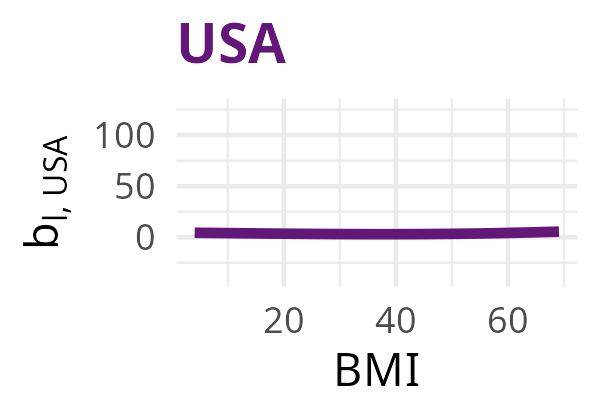
\includegraphics[width=0.19\textwidth]{figures/bs-tensor/fig-tensor-USA.png}}
  {\transparent{0.2}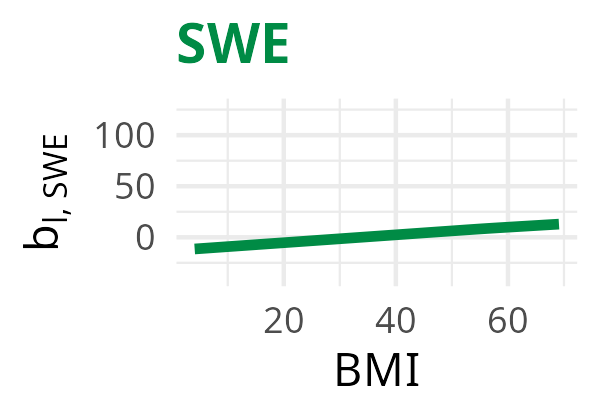
\includegraphics[width=0.19\textwidth]{figures/bs-tensor/fig-tensor-SWE.png}}
  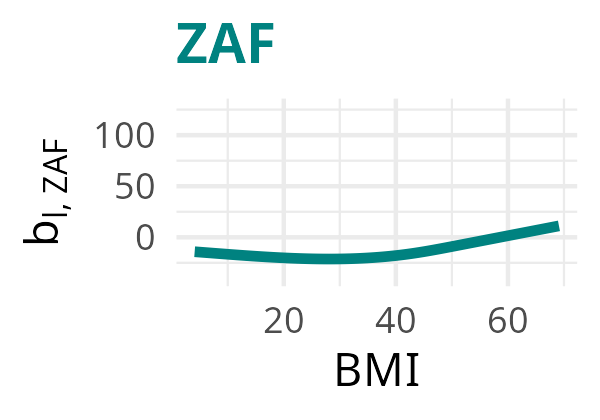
\includegraphics[width=0.19\textwidth]{figures/bs-tensor/fig-tensor-ZAF.png}
  {\transparent{0.2}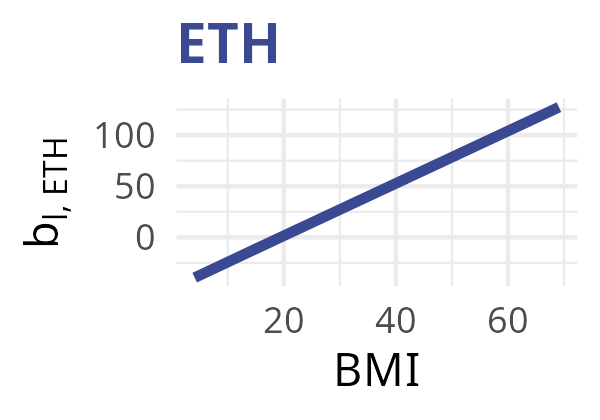
\includegraphics[width=0.19\textwidth]{figures/bs-tensor/fig-tensor-ETH.png}}
  \addtocounter{framenumber}{-1}
\end{frame}

\begin{frame}{(Row-wise) tensor product (RWTP) base learner}
  Example:
  \begin{itemize}
    \item $b_k$ encodes the country: $g_k(x) = (\mathds{1}_{\{x = 1\}}, \dots, \mathds{1}_{\{x = G\}})^\tran$
    \item $b_l$ uses a B-spline basis for BMI: $g_l(x) = (B_{k,1}(x), \dots, B_{k,d_k}(x))^\tran$
  \end{itemize}
  $$
    \design_k \odot \design_l = \tiny\begin{blockarray}{ccccc}
      \color[HTML]{EE0000}g_{k,GER} & \color[HTML]{631879}g_{k,USA} & \color[HTML]{008B45}g_{k,SWE} & \color[HTML]{008280}g_{k,ZAF} & \color[HTML]{3B4992}g_{k,ETH}\\
    \begin{block}{(ccccc)}
      \phantom{x}\\
      \color{lightgray}0 & \color{black}\bm{g_l(x^{(1)})} & \color{lightgray}0 & \color{lightgray}0 & \color{lightgray}0 \\
      \color{lightgray}0 & \color{lightgray}0 & \color{lightgray}0 & \color{lightgray}0 & \color{black}\bm{g_l(x^{(2)})} \\
      \color{black}\bm{g_l(x^{(3)})} & \color{lightgray}0 & \color{lightgray}0 & \color{lightgray}0 & \color{lightgray}0 \\
      \color{lightgray}\vdots & \color{lightgray}\vdots & \color{lightgray}\vdots & \color{lightgray}\vdots & \color{lightgray}\vdots \\
      \color{lightgray}0 & \color{lightgray}0 & \color{black}\bm{g_l(x^{(73)})} & \color{lightgray}0 & \color{lightgray}0 \\
      \color{lightgray}0 & \color{lightgray}0 & \color{lightgray}0 & \color{black}\bm{g_l(x^{(74)})} & \color{lightgray}0 \\
      \color{lightgray}0 & \color{lightgray}0 & \color[HTML]{008B45}\bm{g_l(x^{(75)})} & \color{lightgray}0 & \color{lightgray}0 \\
      \phantom{x}\\
    \end{block}
  \end{blockarray}
  $$
  \normalsize
  {\transparent{0.2}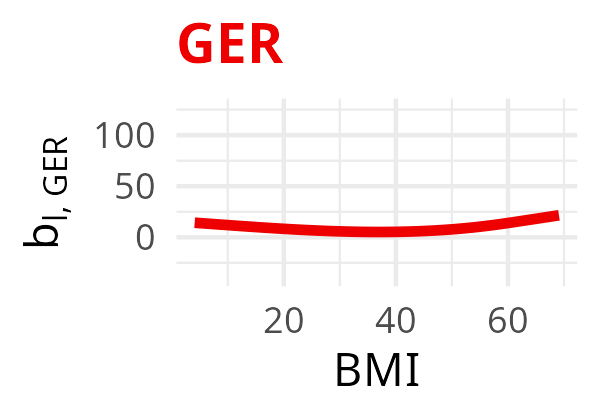
\includegraphics[width=0.19\textwidth]{figures/bs-tensor/fig-tensor-GER.png}}
  {\transparent{0.2}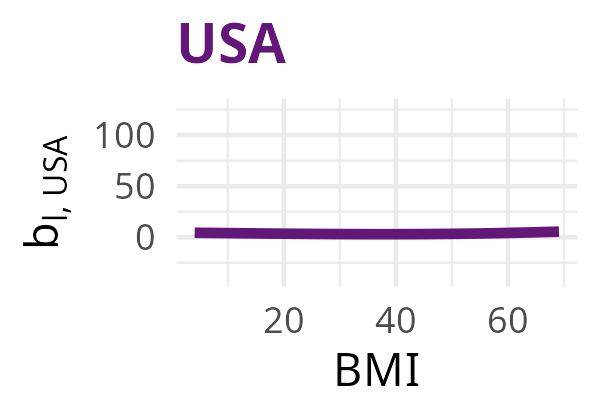
\includegraphics[width=0.19\textwidth]{figures/bs-tensor/fig-tensor-USA.png}}
  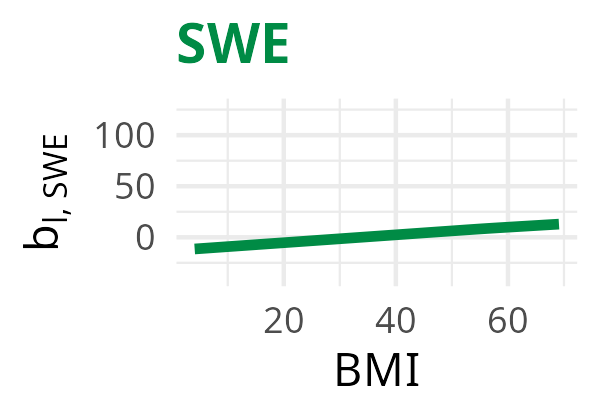
\includegraphics[width=0.19\textwidth]{figures/bs-tensor/fig-tensor-SWE.png}
  {\transparent{0.2}\includegraphics[width=0.19\textwidth]{figures/bs-tensor/fig-tensor-ZAF.png}}
  {\transparent{0.2}\includegraphics[width=0.19\textwidth]{figures/bs-tensor/fig-tensor-ETH.png}}
  \addtocounter{framenumber}{-1}
\end{frame}

\begin{frame}{(Row-wise) tensor product (RWTP) base learner}
  \begin{itemize}
    \item Categoric - numeric base learner combination:
      \begin{figure}
        \centering
        \includegraphics[width=0.5\textwidth]{figures/bs-tensor/fig-cat-num.png}
      \end{figure}
    \item Numeric - numeric base learner combination:
      \begin{figure}
        \centering
        \includegraphics[width=0.5\textwidth]{figures/bs-tensor/fig-num-num.png}
      \end{figure}
  \end{itemize}
\end{frame}


%\fSlide{Component-wise gradient boosting}{Fitting process}

%
\begin{frame}{Example: Life expectancy (nonlinear)}
	\begin{figure}
		\centering
		\includegraphics[width=\textwidth]{figures/cwb-anim/fig-iter-0001.png}
	\end{figure}
	\addtocounter{framenumber}{0}
\end{frame}


\begin{frame}{Example: Life expectancy (nonlinear)}
	\begin{figure}
		\centering
		\includegraphics[width=\textwidth]{figures/cwb-anim/fig-iter-0002.png}
	\end{figure}
	\addtocounter{framenumber}{-1}
\end{frame}


\begin{frame}{Example: Life expectancy (nonlinear)}
	\begin{figure}
		\centering
		\includegraphics[width=\textwidth]{figures/cwb-anim/fig-iter-0005.png}
	\end{figure}
	\addtocounter{framenumber}{-1}
\end{frame}


\begin{frame}{Example: Life expectancy (nonlinear)}
	\begin{figure}
		\centering
		\includegraphics[width=\textwidth]{figures/cwb-anim/fig-iter-0010.png}
	\end{figure}
	\addtocounter{framenumber}{-1}
\end{frame}


\begin{frame}{Example: Life expectancy (nonlinear)}
	\begin{figure}
		\centering
		\includegraphics[width=\textwidth]{figures/cwb-anim/fig-iter-0015.png}
	\end{figure}
	\addtocounter{framenumber}{-1}
\end{frame}


\begin{frame}{Example: Life expectancy (nonlinear)}
	\begin{figure}
		\centering
		\includegraphics[width=\textwidth]{figures/cwb-anim/fig-iter-0017.png}
	\end{figure}
	\addtocounter{framenumber}{-1}
\end{frame}


\begin{frame}{Example: Life expectancy (nonlinear)}
	\begin{figure}
		\centering
		\includegraphics[width=\textwidth]{figures/cwb-anim/fig-iter-0018.png}
	\end{figure}
	\addtocounter{framenumber}{-1}
\end{frame}


\begin{frame}{Example: Life expectancy (nonlinear)}
	\begin{figure}
		\centering
		\includegraphics[width=\textwidth]{figures/cwb-anim/fig-iter-0020.png}
	\end{figure}
	\addtocounter{framenumber}{-1}
\end{frame}


\begin{frame}{Example: Life expectancy (nonlinear)}
	\begin{figure}
		\centering
		\includegraphics[width=\textwidth]{figures/cwb-anim/fig-iter-0023.png}
	\end{figure}
	\addtocounter{framenumber}{-1}
\end{frame}


\begin{frame}{Example: Life expectancy (nonlinear)}
	\begin{figure}
		\centering
		\includegraphics[width=\textwidth]{figures/cwb-anim/fig-iter-0024.png}
	\end{figure}
	\addtocounter{framenumber}{-1}
\end{frame}


\begin{frame}{Example: Life expectancy (nonlinear)}
	\begin{figure}
		\centering
		\includegraphics[width=\textwidth]{figures/cwb-anim/fig-iter-0030.png}
	\end{figure}
	\addtocounter{framenumber}{-1}
\end{frame}


\begin{frame}{Example: Life expectancy (nonlinear)}
	\begin{figure}
		\centering
		\includegraphics[width=\textwidth]{figures/cwb-anim/fig-iter-0050.png}
	\end{figure}
	\addtocounter{framenumber}{-1}
\end{frame}


\begin{frame}{Example: Life expectancy (nonlinear)}
	\begin{figure}
		\centering
		\includegraphics[width=\textwidth]{figures/cwb-anim/fig-iter-0070.png}
	\end{figure}
	\addtocounter{framenumber}{-1}
\end{frame}


\begin{frame}{Example: Life expectancy (nonlinear)}
	\begin{figure}
		\centering
		\includegraphics[width=\textwidth]{figures/cwb-anim/fig-iter-0088.png}
	\end{figure}
	\addtocounter{framenumber}{-1}
\end{frame}


\begin{frame}{Example: Life expectancy (nonlinear)}
	\begin{figure}
		\centering
		\includegraphics[width=\textwidth]{figures/cwb-anim/fig-iter-0089.png}
	\end{figure}
	\addtocounter{framenumber}{-1}
\end{frame}


\begin{frame}{Example: Life expectancy (nonlinear)}
	\begin{figure}
		\centering
		\includegraphics[width=\textwidth]{figures/cwb-anim/fig-iter-0090.png}
	\end{figure}
	\addtocounter{framenumber}{-1}
\end{frame}


\begin{frame}{Example: Life expectancy (nonlinear)}
	\begin{figure}
		\centering
		\includegraphics[width=\textwidth]{figures/cwb-anim/fig-iter-0110.png}
	\end{figure}
	\addtocounter{framenumber}{-1}
\end{frame}


\begin{frame}{Example: Life expectancy (nonlinear)}
	\begin{figure}
		\centering
		\includegraphics[width=\textwidth]{figures/cwb-anim/fig-iter-0130.png}
	\end{figure}
	\addtocounter{framenumber}{-1}
\end{frame}


\begin{frame}{Example: Life expectancy (nonlinear)}
	\begin{figure}
		\centering
		\includegraphics[width=\textwidth]{figures/cwb-anim/fig-iter-0150.png}
	\end{figure}
	\addtocounter{framenumber}{-1}
\end{frame}



%\begin{frame}{Component-wise gradient boosting -- Example}
%	\begin{figure}
%		\centering
%		\includegraphics[width=\textwidth]{figures/cwb-anim/fig-iter-0150.png}
%	\end{figure}
%	\addtocounter{framenumber}{-1}
%\end{frame}


\section{Efficiency}

\begin{frame}{About -- Problems of CWB}

  Computational complexity in terms of memory and runtime efficiency.
  \begin{itemize}
    \item \textbf{W.r.t. runtime:}
    \begin{itemize}
      \item Training CWB requires to (theoretically) calculate $(\design_k^\tran \design_k + \bm{K}_\blk)^{-1}\design_k^\tran \rmm$ for all $k = 1, \dots, K$ and $M$ iterations.
      \item The computational load is tremendously reduced by pre-calculating the Cholesky decompositions of $\design_k^\tran \design_k + \bm{K}_\blk$ for all $k$ as iteration independent part and to re-cycle these matrices in each iteration.
      \item Nevertheless, for big $K$ and $M$ this remains very costly and time consuming.
    \end{itemize}
    \item[] $\Rightarrow$ Fitting the algorithm can take too much time.
  \end{itemize}
\end{frame}

\begin{frame}{About -- Problems of CWB}

  Computational complexity in terms of memory and runtime efficiency.
  \begin{itemize}
    \item \textbf{W.r.t. memory:}
    \begin{itemize}
      \item Each base learner requires to store a design matrix.
      \item For example, using B-splines, it is common to to store an $n\times 24$ matrix (for $20$ knots, and cubic basis functions) for one numerical feature.
    \end{itemize}
    \item[] $\Rightarrow$ The RAM is filled very fast.
  \end{itemize}
\end{frame}

\begin{frame}{Efficiency problems of CWB}

  Computational complexity in terms of memory and runtime efficiency.
  \begin{itemize}
    \item \textbf{W.r.t. runtime:} Fitting the algorithm can take too much time.
    \item \textbf{W.r.t. memory:} The RAM is filled very fast.
  \end{itemize}
  \begin{itemize}
    \item[$\Rightarrow$] Less attractive or infeasible for medium- to large-scale applications.
  \end{itemize}
\end{frame}

\begin{frame}{Publication [2]}
  \vspace{-0.2cm}
  \begin{figure}
    \centering
    \frame{\includegraphics[width=0.7\textwidth]{figures/fig-cacb-paper.png}}
  \end{figure}
  \vspace{-0.4cm}

  \textbf{Aims:}
  \begin{itemize}
    \item
      \textbf{Accelerate the fitting process} of CWB by incorporating Nesterovs momentum.
    \item
      \textbf{Reduce the memory load} by implementing a more efficient data representation for the design matrices.
  \end{itemize}
\end{frame}

\fSlide{Efficiency}{Accelerating component-wise boosting}

\begin{frame}{Accelerating component-wise boosting -- Idea}

  \textbf{Gradient descent:}

  \vspace{0.2cm}
  {\small
  \begin{tabular}{ccc}
    Parameter space & & Function space \\[0.3cm]
    $\tbh^{[m+1]} = \tbh^{[m]} + \nu \nabla_{\tb}\riske(\fh(. | \tbh^{[m]}) | \D)$ & $\Rightarrow$ & $\fh^{[m+1]} = \fmh + \nu \hat{b}^{[m]}$
  \end{tabular}}
  \vspace{0.4cm}

  \textbf{Nesterovs momentum:}

  \vspace{0.2cm}
  {\small
  \begin{tabular}{ccc}
    Parameter space & & Function space \\[0.3cm]
    $\bm{u}^{[m]} = \nabla_{\tb}\riske(\fh(. | \tbh^{[m]} - \gamma \hat{\bm{\vartheta}}^{[m-1]}) | \D)$ &  & \\
    $\hat{\bm{\vartheta}}^{[m]} = \gamma \hat{\bm{\vartheta}}^{[m-1]} + \nu \bm{u}^{[m]}$ & $\Rightarrow$ & ??? \\
    $\tbh^{[m+1]} = \tbh^{[m]} + \hat{\bm{\vartheta}}^{[m]}$ & &
  \end{tabular}}
  \vspace{0.2cm}

  \begin{itemize}
  \item[$\Rightarrow$] \textbf{Idea:} Use Nesterovs momentum and adjust it for functional updates and CWB.
  \end{itemize}

\end{frame}

\begin{frame}{Accelerating component-wise boosting -- Idea}

  \begin{itemize}
    \item
      Using momentum and Nesterovs momentum was first proposed by \cite{biau2019accelerated} and refined in an algorithm called Accelerated Gradient Boosting Machine (AGBM) by \cite{lu2020accelerating}:
      \begin{align*}
      g^{[m]} &= (1 - \theta_m) f^{[m]} + \theta_m h^{[m]}\\
      f^{[m+1]} &= g^{[m]} + \eta b^{[m]} \\
      h^{[m+1]} &= h^{[m]} + \eta / \theta_m b^{[m]}_{\text{cor}}
      \end{align*}
    \item
      Incorporate these adjustments into CWB and make sure all advantages are preserved.
  \end{itemize}
  %\textbf{Memory reduction}
  %\begin{itemize}
    %\item
      %Reduce the memory consumption of CWB
    %\item
      %Apply binning~\citep{} to reduce the matrix size of each base learner and ensure
    %\item
      %Side effect: The runtime also gets better.
  %\end{itemize}

\end{frame}

\begin{frame}{Base learners in AGBM}
  \begin{itemize}
    \item
      \(b^{[m]}\) is fit to pseudo residuals \(\rmm\) w.r.t.
      \(\hat{g}^{[m-1]}\) instead of \(\fmh\)

    \item
      AGBM introduces a second base learner $b^{[m]}_{\text{cor}}$ that is fitted to error-corrected pseudo residuals:
      \[c^{[m](i)} = \rmi + \frac{m}{m+1}(c^{[m-1](i)} - \hat{b}_{\text{cor}}^{[m-1]}(\xi)),\]
      with \(i = 1, \dots, n\), if \(m > 1\) and \(\bm{c}^{[m]} = \rmm\) if
      \(m = 0\).

    \item[] $\Rightarrow$ Each iteration adds not one but two base learners $b^{[m]}$ and $b^{[m]}_{\text{cor}}$:
      \begin{itemize}
        \item $b^{[m]}_{\text{cor}}$ defines the momentum sequence to accelerate the fitting into the direction of the error-corrected pseudo residuals
        \item Computing a second base learner also means two double the runtime for the same number of iterations.
      \end{itemize}
  \end{itemize}
\end{frame}


\begin{frame}{Accelerating component-wise boosting}
  \citet{schalk2022accelerated} introduces an accelerated CWB (ACWB)
  version by incorporating these adaptions to CWB, therefore:

  \begin{itemize}
    \item
      Both base learners, \(b^{[m]}\) and \(b^{[m]}_{\text{cor}}\), are the
      result of a selection process that chooses one of \(b_1, \dots, b_K\)
      w.r.t. to the minimal SSE on the respective pseudo residuals \(\rmm\)
      and \(\bm{c}^{[m]}\).
    \item
      Update the estimated parameters accordingly to allow the estimation of
      partial feature effects.
  \end{itemize}
  Considering these points allows to maintain all advantages of CWB in
  ACWB. Details are outlined in the publication.
\end{frame}

\begin{frame}{Hybrid component-wise boosting}
  \begin{itemize}
    \item
      It was proven by \citet{lu2020accelerating}, that ACWB can overfit if
      not stopped early.
    \item
      Therefore, a hybrid CWB (HCWB) approach combines ACWB for an accelerated fitting in the beginning and CWB
      to fine-tune the model:
  \end{itemize}

  \begin{figure}
    \centering
    \includegraphics[width=0.6\textwidth]{figures/fig-HCWB.pdf}
  \end{figure}
\end{frame}

\fSlide{Efficiency}{Reduced memory consumption in component-wise boosting}

\begin{frame}{Base learner design matrix}
  \begin{itemize}
    \item
      Each base learner \(b_1, \dots, b_K\) requires to build a design
      matrix \(\bm{Z}_k\in\mathbb{R}^{n\times d_k}\) based on the feature
      vector \(\bm{x}_k\).
    \item
      For example:
  \end{itemize}

  \begin{minipage}{0.85\textwidth}
    {\tiny $\underbrace{\begin{pmatrix} 234 \\ 73 \\ 498 \\ \vdots \\ 112 \\ 261 \\ 343 \end{pmatrix}}_{= \bm{x}_{k}\in\R^n}$}
    {\normalsize $\Rightarrow$}
    {\tiny $\underbrace{
      \begin{pmatrix}
        \color{lightgray}0.00 & \color{lightgray}0.00 & \color{lightgray}0.00 & \color{black}0.07 & \color{black}0.62 & \color{black}0.31 &
          \color{lightgray}0.00 & \color{lightgray}0.00 & \color{lightgray}0.00 & \color{lightgray}0.00\color{black}\\
        \color{lightgray}0.00 & \color{black}0.20 & \color{black}0.66 & \color{black}0.14 & \color{lightgray}0.00 & \color{lightgray}0.00 &
          \color{lightgray}0.00 & \color{lightgray}0.00 & \color{lightgray}0.00 & \color{lightgray}0.00\color{black}\\
        \color{lightgray}0.00 & \color{lightgray}0.00 & \color{lightgray}0.00 & \color{lightgray}0.00 & \color{lightgray}0.00 & \color{lightgray}0.00 &
          \color{lightgray}0.00 & \color{black}0.17 & \color{black}0.67 & \color{black}0.17\color{black}\\
        \color{black}\vdots & \color{black}\vdots & \color{black}\vdots & \color{black}\vdots & \color{black}\vdots & \color{black}\vdots & \color{black}\vdots &
          \color{black}\vdots & \color{black}\vdots & \color{black}\vdots\\
        \color{lightgray}0.00 & \color{black}0.02 & \color{black}0.48 & \color{black}0.48 & \color{black}0.02 & \color{lightgray}0.00 & \color{lightgray}0.00 &
          \color{lightgray}0.00 & \color{lightgray}0.00 & \color{lightgray}0.00\color{black}\\
        \color{lightgray}0.00 & \color{lightgray}0.00 & \color{lightgray}0.00 & \color{black}0.01 & \color{black}0.40 & \color{black}0.55 & \color{black}0.04 &
          \color{lightgray}0.00 & \color{lightgray}0.00 & \color{lightgray}0.00\color{black}\\
        \color{lightgray}0.00 & \color{lightgray}0.00 & \color{lightgray}0.00 & \color{lightgray}0.00 & \color{lightgray}0.00 & \color{black}0.29 & \color{black}0.63 &
          \color{black}0.08 & \color{lightgray}0.00 & \color{lightgray}0.00\color{black}\\
      \end{pmatrix}
    }_{=\bm{Z}_{k}\in\R^{n\times d_k}\ \text{(B-spline basis)}}$}%\hspace{-0.1cm}
  {\normalsize $\Rightarrow$}
  \end{minipage}\hspace{-0.5cm}
  \begin{minipage}{0.13\textwidth}
    \vspace{-0.3cm}
    \parbox{0.5\linewidth}{\includegraphics[width=2.5cm]{figures/binning/fig-fe.png}}
  \end{minipage}
  \begin{itemize}
    \item[$\Rightarrow$] If $n$ is large, the memory gets filled very fast (especially if $p$ is also large).
  \end{itemize}
\end{frame}

\begin{frame}{Binning}
  \begin{itemize}
    \item
      To reduce the memory consumption, we applied binning to operate on a
      reduced representation of \(\bm{Z}_k\).
    \item
      Binning is a technique that allows to represent the \(n\) values
      \(x_k^{(1)}, \dots, x_k^{(n)}\) of \(\xv_k\) by \(n^\ast < n\) design
      points \(\bm{z}_k = (z_k^{(1)}, \dots, z_k^{(n^\ast)})\).
    \item
      The idea is to assign each \(x_k^{(i)}\) to the closest design point
      \(z_k^{(i)}\) and store the assignment in a map
      \(\text{ind}_k^{(i)}\):
      \(x_k^{(i)} \approx z_k^{(\text{ind}_k^{(i)})}\)
  \end{itemize}

  \begin{center}\includegraphics[width=9cm]{figures/binning/fig-xbin.png} \end{center}
\end{frame}

\begin{frame}{Binning in GLMs}
  \begin{itemize}
    \item
      \citet{lang2014multilevel} used binning to discretize feature vectors
      to increase the efficiency of multilevel structured additive
      regression.
    \item
      \citet{wood2017gigadata} applied binning to fit GAMs to gigadata and
      argue that the best approximation is achieved by setting
      \(n^\ast = \sqrt{n}\).
    \item
      \citet{li2020faster} presented optimized cross-product operations of
      binned design matrices to also speed up the fitting.
  \end{itemize}
\end{frame}

\begin{frame}{Binning in CWB}
  \begin{itemize}
    \item
      Represent numerical features \(\bm{x}_k\) by \(n^\ast\) design points
      \(\bm{z}_k\).
    \item
      Build the design matrix \(\bm{Z}_k^\ast\) based on \(\bm{z}_k\) which
      requires to store \(n^\ast d_k\) values instead of \(nd_k\).
    \item
      Use optimized cross-product operations to estimate the parameters
      \(\tbh_k^{[m]}\) of base learner \(b_k\) to also speed up the fitting.
  \end{itemize}

  \hspace{-0.2cm}
  \begin{minipage}{0.85\textwidth}
    {\tiny $\underbrace{\begin{pmatrix} 7.0 \\ 129.8 \\ 252.5 \\ 375.2 \\ 498.0 \end{pmatrix}}_{= \bm{z}_{k}\in\R^{n^\ast}}$}
  {\normalsize $\Rightarrow$}
  {\tiny $\underbrace{
    \begin{pmatrix}
      \color{black}0.17 & \color{black}0.67 & \color{black}0.17 & \color{lightgray}0.00 & \color{lightgray}0.00 & \color{lightgray}0.00 &
        \color{lightgray}0.00 & \color{lightgray}0.00 & \color{lightgray}0.00 & \color{lightgray}0.00\\
      \color{lightgray}0.00 & \color{lightgray}0.00 & \color{black}0.32 & \color{black}0.61 & \color{black}0.07 & \color{lightgray}0.00 &
        \color{lightgray}0.00 & \color{lightgray}0.00 & \color{lightgray}0.00 & \color{lightgray}0.00\\
      \color{lightgray}0.00 & \color{lightgray}0.00 & \color{lightgray}0.00 & \color{black}0.02 & \color{black}0.48 & \color{black}0.48 &
        \color{black}0.02 & \color{lightgray}0.00 & \color{lightgray}0.00 & \color{lightgray}0.00\\
      \color{lightgray}0.00 & \color{lightgray}0.00 & \color{lightgray}0.00 & \color{lightgray}0.00 & \color{lightgray}0.00 & \color{black}0.07 &
        \color{black}0.61 & \color{black}0.32 & \color{lightgray}0.00 & \color{lightgray}0.00\\
      \color{lightgray}0.00 & \color{lightgray}0.00 & \color{lightgray}0.00 & \color{lightgray}0.00 & \color{lightgray}0.00 & \color{lightgray}0.00 &
        \color{lightgray}0.00 & \color{black}0.17 & \color{black}0.67 & \color{black}0.17
    \end{pmatrix}}_{=\bm{Z}^\ast_{k}\in\R^{n^\ast\times d_k}\ \text{(B-spline basis)}}$}%\hspace{-0.2cm}
  {\normalsize $\Rightarrow$}
  \end{minipage}\hspace{-0.38cm}
  \begin{minipage}{0.13\textwidth}
    \vspace{-0.3cm}
    \parbox{0.5\linewidth}{\includegraphics[width=2.5cm]{figures/binning/fig-fe.png}}
  \end{minipage}
\end{frame}

\begin{frame}{Adaptions to CWB}
  \todo Hier nochmal alles zusammenschreiben, also wieso passt es gut zu CWB, wie wird es eingebaut etc. Hier muss ich etwas länger drüber reden, das ist ja wa sich quasi gemacht habe.
\end{frame}

\begin{frame}{Example: Memory savings}
  Tabelle wie viel Speicher wann gespart wird.
\end{frame}

\fSlide{Efficiency}{Results, summary, and outlook}

\begin{frame}{Runtime comparisons of CWB variants}
  \begin{figure}
    \centering
    \includegraphics[width=\textwidth]{figures/fig-cacb-runtimes.pdf}
  \end{figure}
\end{frame}

\begin{frame}{Benchmark comparisons of CWB variants}
  \begin{figure}
    \centering
    \includegraphics[width=\textwidth]{figures/fig-cacb-benchmark.pdf}
  \end{figure}
\end{frame}

\begin{frame}{Memory consumption for bigger data sets}
  \begin{figure}
    \centering
    \includegraphics[width=\textwidth]{figures/fig-cacb-big-data.pdf}
  \end{figure}
\end{frame}

\begin{frame}{Summary and Outlook}
  \textbf{Summary:}
  \begin{itemize}
    \item
      We incorporated Nesterovs momentum to speed up the fitting time.
    \item
      Binning allows to save memory by a reduced representation and also to speed up the fitting process by using tailored matrix operations.
    \item
      A benchmark showed the effectiveness of these approaches by being significantly faster by achieving the same or better test performance.
  \end{itemize}
  \textbf{Outlook:}
  \begin{itemize}
    \item
      Using array arithmetic to even faster calculate matrix products and the RWTP base learner.
  \end{itemize}
\end{frame}

\section{Distributed computing}

\newcommand{\iSite}{s}
\newcommand{\nSites}{S}
\newcommand{\doH}{\texttt{[H]}\xspace}
\newcommand{\doS}{\texttt{[S]}\xspace}
\newcommand{\algospace}{\hspace{\algorithmicindent}}
\newcommand{\lsite}{\blk_\times}

\begin{frame}{Distributed data set}
  Assume the \texttt{Country} column is not present in the data set and each country holds a its own partition:\vspace{-0.3cm}
  {\tiny
  \begin{table}
  \centering
  \begin{tabular}[t]{cccccc}
  \toprule
    \textbf{Life.expectancy} & {\color{lightgray}\textbf{Country}} & \textbf{Year} & \textbf{BMI} & \textbf{Adult.Mortality} & \textbf{Data set}\\
  \midrule
    51.2 & {\color{lightgray}ETH} & 2000 & 12.3 & 391 & \multirow{3}{*}{\color[HTML]{3B4992}\normalsize$\mathcal{D}_1$}\\
    {\tiny$\vdots$} & {\tiny\color{lightgray}$\vdots$} & {\tiny$\vdots$} & {\tiny$\vdots$} & {\tiny$\vdots$}\\
    64.8 & {\color{lightgray}ETH} & 2015 & 17.6 & 225\\ \hline
    78.0 & {\color{lightgray}GER} & 2000 & 55.1 & 95 & \multirow{3}{*}{\color[HTML]{EE0000}\normalsize$\mathcal{D}_2$}\\
    {\tiny$\vdots$} & {\tiny\color{lightgray}$\vdots$} & {\tiny$\vdots$} & {\tiny$\vdots$} & {\tiny$\vdots$}\\
    81.0 & {\color{lightgray}GER} & 2015 & 62.3 & 68\\ \hline
    79.6 & {\color{lightgray}SWE} & 2000 & 52.8 & 73 & \multirow{3}{*}{\color[HTML]{008B45}\normalsize$\mathcal{D}_3$}\\
    {\tiny$\vdots$} & {\tiny\color{lightgray}$\vdots$} & {\tiny$\vdots$} & {\tiny$\vdots$} & {\tiny$\vdots$}\\
    82.4 & {\color{lightgray}SWE} & 2015 & 59.5 & 53\\ \hline
    76.8 & {\color{lightgray}USA} & 2000 & 6.1  & 114 & \multirow{3}{*}{\color[HTML]{631879}\normalsize$\mathcal{D}_4$}\\
    {\tiny$\vdots$} & {\tiny\color{lightgray}$\vdots$} & {\tiny$\vdots$} & {\tiny$\vdots$} & {\tiny$\vdots$}\\
    79.3 & {\color{lightgray}USA} & 2015 & 69.6 & 13\\ \hline
    57.3 & {\color{lightgray}ZAF} & 2000 & 4.1 & 397 & \multirow{3}{*}{\color[HTML]{008280}\normalsize$\mathcal{D}_5$}\\
    {\tiny$\vdots$} & {\tiny\color{lightgray}$\vdots$} & {\tiny$\vdots$} & {\tiny$\vdots$} & {\tiny$\vdots$}\\
    62.9 & {\color{lightgray}ZAF} & 2015 & 51.1 & 328\\
  \bottomrule
  \end{tabular}
  \end{table}}
  $\Rightarrow$ Due to privacy reasons, it is not allowed to share and merge these data sets to $\mathcal{D} = \cup_{s=1}^S \mathcal{D}_s$.
\end{frame}

\begin{frame}{Distributed data set}
  Assume the \texttt{Country} column is not present in the data set and each country holds a its own partition:
  \vspace{-0.2cm}
  \begin{figure}
    \centering
    \includegraphics[width=0.45\textwidth]{figures/weltkarte.png}
  \end{figure}
  \vspace{-0.5cm}
  \begin{itemize}
    \item We are looking at \textbf{horizontally partitioned data}: Each site holds the same features but different observations.
    \item \textbf{Vertically partitioned data}: Each site has the same observations but different features.
  \end{itemize}
  $\Rightarrow$ Can we still fit a model with CWB?
\end{frame}

\begin{frame}{Setup}
  \begin{itemize}
    \item $\nSites$ sites, each exclusively hold a data set $\mathcal{D}_\iSite$
    \item A host in the middle controls the communication with the sites, the sites cannot communicate with each other.
    \item The host is the volnurable component since it can be highjacket and access to the communicated data is ont out of question.
    \item Hence, the communicated data from the sites must ensure privacy of the original data sets.
    \item Often applies to sensitive data, e.g., most data sets with private information about individuals.
  \end{itemize}
  What is allowed to be shared?
  \begin{itemize}
    \item Aggregated data that does not allow to re-construct parts of the original data set.
    \item Encrypted data (e.g. via homomorphic encription~\citep{gentry2009fully}).
  \end{itemize}
\end{frame}

\begin{frame}{Publication [4]}
  \vspace{-0.2cm}
  \begin{figure}
    \centering
    \frame{\includegraphics[width=0.55\textwidth]{figures/fig-paper-dcwb.png}}
  \end{figure}
  \vspace{-0.2cm}
  \textbf{Aims:}
  \begin{itemize}
    \item
      Provide a \textbf{distributed and lossless CWB algorithm}: \[\operatorname{distCWB}(\mathcal{D}_1, \dots, \mathcal{D}_\nSites) = \operatorname{CWB}(\mathcal{D})\]
    \item
      \textbf{Allow for site-specific corrections} get a deeper understanding of the distributed data.
  \end{itemize}

\end{frame}

\begin{frame}{Site-specific vs. main effects}
  %\todo Auf main oder shared festlegen?
  \begin{itemize}
    \item
      \textbf{Reminder:} CWB can be used to fit a GAM $f(\xv) = f_0 + \sum_{k=1}^K b_k(\xv)$ with the base learners $b_k$ as additive terms.
    \item
      In the distributed setup, we denote $b_k$ as shared or main effect that is equal between all sites.

    \item
      Furhter, these effects are extended by site-specific effects $b_{k,s}$ that allow a site-specific correction of the shared effect.
  \end{itemize}

  The final model assembles both, common shared and site specific effects:
  \[f(\xv) = f_0 + \sum_{k=1}^K\left(b_k(\xv) + \sum_{s=1}^S b_{k,s}(\xv)\right) = f_0 + \sum_{k=1}^K \underbrace{b_k(\xv)}_{\text{main effect}} + \underbrace{(b_k \odot b_0)(\xv)}_{\text{site-specific effect}}\]

  This structure is equal to CWB with base learner $b_k$, $k = 1, \dots, K$, and RWTP base learners $b_k \odot b_0$, $k = 1, \dots, K$, with $b_0$ a latent one hot encoded categorical base learner modelling the $S$ sites.
\end{frame}

\begin{frame}{Bla}
  \todo Genau auf shared und site-specific effects eingehen. Was bedeutet das?
\end{frame}

%\begin{frame}{Component-wise boosting as fitting engine}
  %\begin{itemize}
    %\item CWB can be used to fit the a model related to equation xyz
    %\item Simply achieved by:
      %\begin{itemize}
        %\item Assuming a latent categorical feature for the sites
        %\item Use one base learner for the features to model the whole feature effect
        %\item and a tensor product base learner between all fetures and the latent categorical feature to estimate site-specific effects.
      %\end{itemize}
    %\item Adaption to distributed data requires to fit the base learners to distributed data.
  %\end{itemize}
%\end{frame}

\fSlide{Distributed CWB}{Estimation of main effects}

\begin{frame}{Estimation of main effects}
  %We restricted CWB to fit $b_k$ using OLS by $\tbh_k = (\design_k^\tran \design_k)^{-1}\design_k^\tran \rmm$.
  \begin{algorithm}[H]
  \scriptsize
  \caption{Vanilla CWB algorithm}
  %\vspace{0.15cm}
  \hspace*{\algorithmicindent} \textbf{Input} Train data $\D$, learning rate $\nu$, number of boosting iterations $M$, loss\\
  \hspace*{\algorithmicindent} \phantom{\textbf{Input} } function $L$, base learners $b_1, \dots, b_\blK$\\
  \hspace*{\algorithmicindent} \textbf{Output} Model $\fh = \fmh[M]$\vspace{0.1cm}
  \hrule
  \begin{algorithmic}[1]
  \Procedure{$\operatorname{CWB}$}{$\D,\nu,M,L,b_1, \dots, b_\blK$}
      \State \tikzmk{A}Initialize: $f_0 = \fh^{[0]}(\xv) = \argmin_{c\in\mathcal{Y}}\riske(c|\D)$
      \While{$m \leq M$}
          \State $\rmi = -\left.\pd{\Lxyi}{f(\xi)}\right|_{f = \fmdh},\ \ \forall i \in \{1, \dots, n\}$
          \For{$\blk \in \{1, \dots, \blK\}$}\tikzmk{B}\boxtrans
              \State \tikzmk{A}$\tbmh_\blk = \left(\design_\blk^\tran \design_\blk + \bm{K}_\blk\right)^{-1} \design^\tran_\blk \rmm$ \quad {\color{red} $\bm{\leftarrow}$ \textbf{Distribute}}\tikzmk{B}\boxittwo{olivedrab}
              \State \tikzmk{A}$\sse_\blk = \sum_{i=1}^n(\rmi - b_\blk(\xi | \tbmh_\blk))^2$
          \EndFor
          \State $\blk^{[m]} = \argmin_{\blk\in\{1, \dots, \blK\}} \sse_\blk$
          \State $\fmh(\xv) = \fmdh(\xv) + \nu b_{\blk^{[m]}} (\xv | \tbmh_{\blk^{[m]}})$\tikzmk{B}\boxtrans
      \EndWhile
      \State \textbf{return} $\fh = \fh^{[M]}$
  \EndProcedure
  \end{algorithmic}
  \end{algorithm}
\end{frame}

\begin{frame}{Estimation of main effects}
  \begin{itemize}
    \item Each site holds a design matrix for the $k$\th base learner: $\design_{k,\iSite}$ and a slice of the pseudo residuals: $\rmm_\iSite$
  \end{itemize}
  \tikz[remember picture, overlay] \node[anchor=center] at ($(current page.center)-(0,1.1)$) {\includegraphics[width=0.7\textwidth]{figures/distr-lm-iter1.png}};
  %\begin{figure}
    %\centering
    %\includegraphics[width=0.6\textwidth]{figures/distr-lm-iter1.png}
  %\end{figure}
\end{frame}

\begin{frame}{Estimation of main effects}
  \begin{itemize}
    \item Each site calculates $\bm{F}_{k,\iSite} = \design_{k,\iSite}^\tran \design_{k,\iSite}$ and $\bm{u}^{[m]}_{k,\iSite} = \bm{Z}^\tran_{k,\iSite}\rmm_k$.
  \end{itemize}
  \tikz[remember picture, overlay] \node[anchor=center] at ($(current page.center)-(0,1.1)$) {\includegraphics[width=0.7\textwidth]{figures/distr-lm-iter2.png}};
  %\begin{figure}
    %\centering
    %\includegraphics[width=0.6\textwidth]{figures/distr-lm-iter2.png}
  %\end{figure}
	\addtocounter{framenumber}{-1}%
\end{frame}

\begin{frame}{Estimation of main effects}
  \begin{itemize}
    \item The sites are allowed to communicate $\bm{F}_{k,\iSite}$ and $\bm{u}_{k,\iSite}^{[m]}$ as long as \enquote{enough observations} are used. The host calculates $\bm{F}_k = \sum_{\iSite = 1}^\nSites \bm{F}_{k,\iSite}$ and $\bm{u}_k^{[m]} = \sum_{\iSite = 1}^\nSites \bm{u}_{k,\iSite}^{[m]}$.
  \end{itemize}
  \tikz[remember picture, overlay] \node[anchor=center] at ($(current page.center)-(0,1.1)$) {\includegraphics[width=0.7\textwidth]{figures/distr-lm-iter3.png}};
  %\begin{figure}
    %\centering
    %\includegraphics[width=0.6\textwidth]{figures/distr-lm-iter3.png}
  %\end{figure}
\end{frame}
	\addtocounter{framenumber}{-1}%

\begin{frame}{Estimation of main effects}
  \begin{itemize}
    \item Finally, the host can estimate $\tbh_k^{[m]} = (\bm{F}_k + \penMat_k)^{-1} \bm{u}_k$.
  \end{itemize}
  \tikz[remember picture, overlay] \node[anchor=center] at ($(current page.center)-(0,1.1)$) {\includegraphics[width=0.7\textwidth]{figures/distr-lm-iter4.png}};
  %\begin{figure}
    %\centering
    %\includegraphics[width=0.6\textwidth]{figures/distr-lm-iter4.png}
  %\end{figure}
	\addtocounter{framenumber}{-1}%
\end{frame}

\begin{frame}{Estimation of main effects}
  \begin{algorithm}[H]
    \footnotesize
    \caption{Distributed Effect Estimation~\citep{karr2005secure}.\\
    The line prefixes \doS and \doH indicate whether the operation is conducted at the sites (\doS) or at the host (\doH).}\label{algo:lm-distr}
    \vspace{0.15cm}
    \hspace*{\algorithmicindent} \textbf{Input} Sites design matrices $\design_{k,1}, \dots, \design_{k,\nSites}$, response vectors $\rmm_1, \dots, \rmm_\nSites$ and\\
    \hspace*{\algorithmicindent} \phantom{\textbf{Input} }an optional penalty matrix $\penMat_k$.\\
    \hspace*{\algorithmicindent} \textbf{Output} Estimated parameter vector $\tbh_k$.\vspace{0.15cm}
    \hrule
    \begin{algorithmic}[1]
      \Procedure{$\operatorname{distFit}$}{$\design_{k,1}, \dots, \design_{k,\nSites}, \rmm_1, \dots, \rmm_\nSites, \penMat_k$}
        \For{$\iSite \in \{1, \dots, \nSites\}$}
          \State \doS $\bm{F}_{k,\iSite} = \design_{k,\iSite}^\tran \design_{k,\iSite}$
          \State \doS $\bm{u}_{k,\iSite} = \design_{k,\iSite}^\tran \rmm_\iSite$
          \State \doS Communicate $\bm{F}_{k,\iSite}$ and $\bm{u}_{k,\iSite}$ to the host
        \EndFor
        \State \doH $\bm{F}_k = \sum_{\iSite=1}^\nSites \bm{F}_{k,\iSite} + \penMat_k$
        \State \doH $\bm{u}_k = \sum_{\iSite=1}^\nSites \bm{u}_{k,\iSite}$
        \State \doH \textbf{return} $\tbh_k = \bm{F}_k^{-1}\bm{u}_k$
      \EndProcedure
    \end{algorithmic}
  \end{algorithm}
  \normalsize
\end{frame}

\begin{frame}{Estimation of main effects}
  Substituting $\tbmh_\blk = \left(\design_\blk^\tran \design_\blk + \bm{K}_\blk\right)^{-1} \design^\tran_\blk \rmm$ with $\operatorname{distFit}$ in each iteration $m$ gives a first lossless distributed CWB algorithm.
  \begin{algorithm}[H]
  \scriptsize
  \caption{Vanilla CWB algorithm}
  %\vspace{0.15cm}
  \hspace*{\algorithmicindent} \textbf{Input} Train data $\D$, learning rate $\nu$, number of boosting iterations $M$, loss\\
  \hspace*{\algorithmicindent} \phantom{\textbf{Input} } function $L$, base learners $b_1, \dots, b_\blK$\\
  \hspace*{\algorithmicindent} \textbf{Output} Model $\fh = \fmh[M]$\vspace{0.1cm}
  \hrule
  \begin{algorithmic}[1]
  \Procedure{$\operatorname{CWB}$}{$\D,\nu,M,L,b_1, \dots, b_\blK$}
      \State \tikzmk{A}Initialize: $f_0 = \fh^{[0]}(\xv) = \argmin_{c\in\mathcal{Y}}\riske(c|\D)$
      \While{$m \leq M$}
          \State $\rmi = -\left.\pd{\Lxyi}{f(\xi)}\right|_{f = \fmdh},\ \ \forall i \in \{1, \dots, n\}$
          \For{$\blk \in \{1, \dots, \blK\}$}\tikzmk{B}\boxtrans
              \State \tikzmk{A}$\tbmh_\blk = \left(\design_\blk^\tran \design_\blk + \bm{K}_\blk\right)^{-1} \design^\tran_\blk \rmm$ \quad {\color{red} $\bm{\leftarrow}$ \textbf{Distribute}}\tikzmk{B}\boxittwo{olivedrab}
              \State \tikzmk{A}$\sse_\blk = \sum_{i=1}^n(\rmi - b_\blk(\xi | \tbmh_\blk))^2$
          \EndFor
          \State $\blk^{[m]} = \argmin_{\blk\in\{1, \dots, \blK\}} \sse_\blk$
          \State $\fmh(\xv) = \fmdh(\xv) + \nu b_{\blk^{[m]}} (\xv | \tbmh_{\blk^{[m]}})$\tikzmk{B}\boxtrans
      \EndWhile
      \State \textbf{return} $\fh = \fh^{[M]}$
  \EndProcedure
  \end{algorithmic}
  \end{algorithm}
\end{frame}

\begin{frame}{Estimation of main effects}
  Substituting $\tbmh_\blk = \left(\design_\blk^\tran \design_\blk + \bm{K}_\blk\right)^{-1} \design^\tran_\blk \rmm$ with $\operatorname{distFit}$ in each iteration $m$ gives a first lossless distributed CWB algorithm.
  \begin{algorithm}[H]
  \scriptsize
  \caption{Distributed CWB algorithm}
  %\vspace{0.15cm}
  \hspace*{\algorithmicindent} \textbf{Input} Site data $\D_1, \dots, \D_K$, learning rate $\nu$, number of boosting iterations $M$, loss\\
  \hspace*{\algorithmicindent} \phantom{\textbf{Input} } function $L$, base learners $b_1, \dots, b_\blK$\\
  \hspace*{\algorithmicindent} \textbf{Output} Model $\fh = \fmh[M]$\vspace{0.1cm}
  \hrule
  \begin{algorithmic}[1]
  \Procedure{$\operatorname{distCWB}$}{$\D_1, \dots, \D_K,\nu,M,L,b_1, \dots, b_\blK$}
      \State \tikzmk{A}Initialize: $f_0 = \fh^{[0]}(\xv) = \argmin_{c\in\mathcal{Y}}\riske(c|\D)$
      \While{$m \leq M$}
          \State $\rmi = -\left.\pd{\Lxyi}{f(\xi)}\right|_{f = \fmdh},\ \ \forall i \in \{1, \dots, n\}$
          \For{$\blk \in \{1, \dots, \blK\}$}\tikzmk{B}\boxtrans
              \State \tikzmk{A}$\tbmh_\blk = \operatorname{distFit(\design_{k,1}, \dots, \design_{k,\nSites}, \rmm_1, \rmm_\nSites, \penMat_k)}$\tikzmk{B}\boxittwo{olivedrab}
              \State \tikzmk{A}$\sse_\blk = \sum_{i=1}^n(\rmi - b_\blk(\xi | \tbmh_\blk))^2$
          \EndFor
          \State $\blk^{[m]} = \argmin_{\blk\in\{1, \dots, \blK\}} \sse_\blk$
          \State $\fmh(\xv) = \fmdh(\xv) + \nu b_{\blk^{[m]}} (\xv | \tbmh_{\blk^{[m]}})$\tikzmk{B}\boxtrans
      \EndWhile
      \State \textbf{return} $\fh = \fh^{[M]}$
  \EndProcedure
  \end{algorithmic}
  \end{algorithm}
\end{frame}



\fSlide{Distributed CWB}{Estimation of site-specific effects}

\begin{frame}{Estimation of site-specific effects}
  \textbf{Example:} Without sharing sensitive data, we want to esitmate site-specific effects (e.g. for \texttt{BMI}):
  \begin{figure}
    \centering
    \includegraphics[width=0.7\textwidth]{figures/fig-site-effects.png}
  \end{figure}
\end{frame}

\begin{frame}{Distributed estimation of site-specific effects}
  Site-specific effects $b_{\lsite} = b_0 \odot b_k$ are equal to a RWTP base learner with latent categorical base learner $b_0$ encoding the sites and the main effect $b_k$:
  \begin{center}
  \begin{tabular}{ccc}
    \includegraphics[align=c,width=0.3\textwidth]{figures/fig-site-effects.png} &
    {\Large $\Rightarrow$} &
    \includegraphics[align=c,width=0.4\textwidth]{figures/bs-tensor/fig-cat-num.png} \\
  \end{tabular}
  \end{center}
  %\begin{itemize}
    %\item Site-specific effects sind etwas "einfacher" als base learner per site zu schätzen
    %\item parametercshätzer teilen
    %\item Zeigen, dass der tensor spline learner einfach als einzelne Fits ausgedrückt werden kann.
  %\end{itemize}
  \begin{align*}
    \tbh_{\lsite}% &= \fitbl(\yv, \D, b_{\lsite})
    &= \left(\design_{\lsite}^\tran \design_{\lsite} +  \penMat_{\lsite}\right)^{-1}\design_{\lsite}^\tran \yv
    \notag \\
    &= \left(\begin{array}{c}
         (\design_{\blk,1}^\tran \design_{\blk,1} + \lambda_0\idMat_{d_\blk} + \penMat_\blk)^{-1} \design_{\blk,1}^\tran \yv_1 \\
         \vdots \\
         (\design_{\blk,\nSites}^\tran \design_{\blk,\nSites} + \lambda_0\idMat_{d_\blk} + \penMat_\blk)^{-1} \design_{l,\nSites}^\tran \yv_\nSites
    \end{array}\right) =
    \left(\begin{array}{c}
      \tbh_{{\lsite}, 1}  \\
      \vdots \\
      \tbh_{{\lsite}, \nSites}
    \end{array}\right)\in\R^{Sd_k}
  \end{align*}
  %\[\tbh_{{\lsite},\iSite} = (\design_{\blk,\iSite}^\tran \design_{\blk,\iSite} + \lambda_0\idMat_{d_\blk} + \penMat_\blk)^{-1} \design_{\blk,\iSite}^\tran \yv_\iSite\]

\end{frame}

\begin{frame}{Estimation of site-specific effects}
  \begin{itemize}
    \item Each site calculates and communicates the site-specific correction $\tbh_{{\lsite},\iSite} = (\design_{\blk,\iSite}^\tran \design_{\blk,\iSite} + \lambda_0\idMat_{d_\blk} + \penMat_\blk)^{-1} \design_{\blk,\iSite}^\tran \yv_\iSite$.
  \end{itemize}
  \tikz[remember picture, overlay] \node[anchor=center] at ($(current page.center)-(0,1.1)$) {\includegraphics[width=0.6\textwidth]{figures/fig-site-effects.png}};
\end{frame}

\begin{frame}{Estimation of site-specific effects}
  \begin{itemize}
    \item Each site calculates and communicates the site-specific correction $\tbh_{{\lsite},\iSite} = (\design_{\blk,\iSite}^\tran \design_{\blk,\iSite} + \lambda_0\idMat_{d_\blk} + \penMat_\blk)^{-1} \design_{\blk,\iSite}^\tran \yv_\iSite$.
  \end{itemize}
  \tikz[remember picture, overlay] \node[anchor=center] at ($(current page.center)-(0,1.1)$) {\includegraphics[width=0.6\textwidth]{figures/fig-site-effects-iter1.png}};
	\addtocounter{framenumber}{-1}%
\end{frame}

\begin{frame}{Estimation of site-specific effects}
  \begin{itemize}
    \item The host collects all site parameters $\tbmh_{{\lsite},1}, \dots, \tbmh_{{\lsite},\nSites}$ to reconstruct the parameter vector $\tbmh_{\lsite}$ of the RWTP base learner $b_{\lsite}$.
  \end{itemize}
  \tikz[remember picture, overlay] \node[anchor=center] at ($(current page.center)-(0,1.1)$) {\includegraphics[width=0.6\textwidth]{figures/fig-site-effects-iter2.png}};
	\addtocounter{framenumber}{-1}%
\end{frame}


\begin{frame}{Estimation of site-specific effects}
  \begin{algorithm}[H]
  \scriptsize
  \caption{Distributed CWB algorithm}\label{algo:dcwb}
  %\vspace{0.15cm}
  \hspace*{\algorithmicindent} \textbf{Input} Site data $\D_1, \dots, \D_K$, learning rate $\nu$, number of boosting iterations $M$, loss\\
  \hspace*{\algorithmicindent} \phantom{\textbf{Input} } function $L$, base learners $b_1, \dots, b_\blK$\\
  \hspace*{\algorithmicindent} \textbf{Output} Model $\fh = \fmh[M]$\vspace{0.1cm}
  \hrule
  \begin{algorithmic}[1]
  \Procedure{$\operatorname{distCWB}$}{$\D_1, \dots, \D_K,\nu,M,L,b_1, \dots, b_\blK$}
      \State \tikzmk{A}Initialize: $f_0 = \fh^{[0]}(\xv) = \argmin_{c\in\mathcal{Y}}\riske(c|\D)$
      \While{$m \leq M$}
          \State $\rmi = -\left.\pd{\Lxyi}{f(\xi)}\right|_{f = \fmdh},\ \ \forall i \in \{1, \dots, n\}$
          \For{$\blk \in \{1, \dots, \blK\}$}\tikzmk{B}\boxtrans
              \State \tikzmk{A}$\tbmh_\blk = \operatorname{distFit(\design_{k,1}, \dots, \design_{k,\nSites}, \rmm_1, \rmm_\nSites, \penMat_k)}$
              \State$\tbmh_{\lsite} = \operatorname{getSiteEffects}(\tbmh_{{\lsite}, 1}, \dots, \tbmh_{{\lsite},\nSites})$\tikzmk{B}\boxittwo{olivedrab}
              \State \tikzmk{A}$\sse_\blk = \sum_{i=1}^n(\rmi - b_\blk(\xi | \tbmh_\blk))^2$\tikzmk{B}\boxtrans
              \State \tikzmk{A}$\sse_{\lsite} = \sum_{i=1}^n(\rmi - b_{\lsite}(\xi | \tbmh_{\lsite}))^2$
          \EndFor
          \State $\blk^{[m]} = \argmin_{\blk\in\{1, \dots, \blK, 1_{\times}, \dots, \blK_{\times}\}} \sse_\blk$\hspace{0.4cm}\tikzmk{B}\boxittwo{olivedrab}
          \State \tikzmk{A}$\fmh(\xv) = \fmdh(\xv) + \nu b_{\blk^{[m]}} (\xv | \tbmh_{\blk^{[m]}})$\tikzmk{B}\boxtrans
      \EndWhile
      \State \textbf{return} $\fh = \fmh$
  \EndProcedure
  \end{algorithmic}
  \end{algorithm}
\end{frame}

\fSlide{Distributed CWB}{Comparisons, summary, and outlook}

\begin{frame}{Putting all together}
  \begin{itemize}
    \item
      Algorithm~\ref{algo:dcwb} must be extended to account for sharing the SSE values from the sites to the host as well as sharing the estimated parameter of the main effects from the host to the sites.
    \item
      The automatic selection process of CWB and additional penalty $\lambda_0$ that is added to the first-order differences of the site-specific effects allows to favor the main effect over the site-specific effects.
    \item
      The algorithm is implemented in DataSHIELD and available on GitHub \footnote[frame,1]{\url{https://github.com/schalkdaniel/dsCWB}}.
  \end{itemize}
\end{frame}


\begin{frame}{Comparisons}
  \begin{itemize}
    \item \textbf{Reminder:} The proposed algorithm is a lossless and distributed pendant to CWB on the merged data.
    \item Instead of benchmarking the algorithm, we compared it with a GAMM fitted with \texttt{mgcv}.
  \end{itemize}
  \begin{figure}
    \centering
    \includegraphics[width=0.9\textwidth]{figures/fig-dcwb-effect-decomposition.pdf}
  \end{figure}
  \vspace{-0.2cm}
  \begin{figure}
    \centering
    \includegraphics[width=0.8\textwidth]{figures/fig-dcwb-effect-comparison.pdf}
  \end{figure}
\end{frame}


\begin{frame}{Summary and outlook}
  \textbf{Summary:}
  \begin{itemize}
    \item
      CWB can be fit to distributed data in a lossless fashion by just relying on aggregated data that do not reveal private information about the used data set.
    \item
      Site-specific effects can be estimated by making use of the structure of a RWTP base learner.
    \item
      The SSE calculation is also done easily ba sharing the SSE per site and aggregating them.
  \end{itemize}
  \textbf{Outlook:}
  \begin{itemize}
    \item Account for vertically and horizontally distributed data.
    \item Reduce the communication costs to speed up the fitting process.
  \end{itemize}
\end{frame}



%%%%% SHORT SUMMARIES, MAX 2 SLIDES ---------------------------------------------------------------%%


\section{Automation}

\begin{frame}{Publication [3]}
  \vspace{-0.2cm}
  \begin{figure}
    \centering
    \frame{\includegraphics[width=0.7\textwidth]{figures/fig-paper-autocwb.png}}
  \end{figure}
  \vspace{-0.4cm}

  \textbf{Aims:}
  \begin{itemize}
    \item
      Interpretable automated ML system with CWB as fitting engine.
    \item
      Assessment of the required complexity and the decision making process.
  \end{itemize}
\end{frame}


\begin{frame}{About}
  \begin{itemize}
    \item Build a model $f = f_{\text{uni}} + f_{\text{pint}} + f_{\text{deep}}$ based on a multi-stage approach with:
      \begin{itemize}
        \item Univariate effects $f_{\text{uni}}$ decomposed into $f_{\text{uni,linear}}$ and $f_{\text{uni,non-linear}}$
        \item Pairwise interactions $f_{\text{pint}}$ with a RWTP base learner
        \item Deeper interactions $f_{\text{deep}}$ with trees
      \end{itemize}
  \end{itemize}
\end{frame}

\begin{frame}{About}
  \begin{itemize}
    \item Build a model $f = f_{\text{uni}} + f_{\text{pint}} + f_{\text{deep}}$ based on a multi-stage approach with:
      \begin{itemize}
        \item Univariate effects $f_{\text{uni}}$ decomposed into $f_{\text{uni,linear}}$ and $f_{\text{uni,non-linear}}$
        \item Pairwise interactions $f_{\text{pint}}$ with a RWTP base learner
        \item Deeper interactions $f_{\text{deep}}$ with trees
      \end{itemize}
    \item \texttt{Autocompboost} wraps \texttt{compboost} with an AutoML pipeline:
      \begin{figure}
        \centering
        \includegraphics[width=0.8\textwidth]{figures/fig-acwb-ml-pipeline.png}
      \end{figure}
  \end{itemize}
	\addtocounter{framenumber}{-1}
\end{frame}

\begin{frame}{About}
  \begin{itemize}
    \item Build a model $f = f_{\text{uni}} + f_{\text{pint}} + f_{\text{deep}}$ based on a multi-stage approach with:
      \begin{itemize}
        \item Univariate effects $f_{\text{uni}}$ decomposed into $f_{\text{uni,linear}}$ and $f_{\text{uni,non-linear}}$
        \item Pairwise interactions $f_{\text{pint}}$ with a RWTP base learner
        \item Deeper interactions $f_{\text{deep}}$ with trees
      \end{itemize}
    \item \texttt{Autocompboost} wraps \texttt{compboost} with an AutoML pipeline:
      \begin{figure}
        \centering
        \includegraphics[width=0.25\textwidth]{figures/fig-acwb-ml-pipeline.png}
      \end{figure}
    \item Using boosting allows to gain a fine grid of the risk improvement for each stage:
      \begin{figure}
        \centering
        \includegraphics[width=0.7\textwidth]{figures/fig-acwb-risk.png}
      \end{figure}
  \end{itemize}
	\addtocounter{framenumber}{-1}
\end{frame}

\begin{frame}{About}
  \begin{itemize}
    \item Build a model $f = f_{\text{uni}} + f_{\text{pint}} + f_{\text{deep}}$ based on a multi-stage approach with:
      \begin{itemize}
        \item Univariate effects $f_{\text{uni}}$ decomposed into $f_{\text{uni,linear}}$ and $f_{\text{uni,non-linear}}$
        \item Pairwise interactions $f_{\text{pint}}$ with a RWTP base learner
        \item Deeper interactions $f_{\text{deep}}$ with trees
      \end{itemize}
    \item \texttt{Autocompboost} wraps \texttt{compboost} with an AutoML pipeline:
      \begin{figure}
        \centering
        \includegraphics[width=0.25\textwidth]{figures/fig-acwb-ml-pipeline.png}
      \end{figure}
    \item Using boosting allows to gain a fine grid of the risk improvement for each stage:
      \begin{figure}
        \centering
        \includegraphics[width=0.25\textwidth]{figures/fig-acwb-risk.png}
      \end{figure}
    \item Explaining the framework is done by using the CWBs interpretation functionality.
  \end{itemize}
	\addtocounter{framenumber}{-1}
\end{frame}




\begin{frame}{Limitation and Outlook}
  \textbf{Limitations:}
  \begin{itemize}
    \item Detecting interactions is done heuristically by a surrogate random forest and hence on a different model class than stage one and two.
    \item It is not clear how switching the model class in stage can revert the effects of stage one and two.

  \end{itemize}
  \textbf{Outlook:}
  \begin{itemize}
    \item Other techniques to detect interactions and simulations to show their effectiveness.
    \item Focus on the third stage. An idea is to orthogonalize $f_{\text{deep}}$ by $f_{\text{uni}} + f_{\text{pint}}$ to ensure that their effects remain untouched.
  \end{itemize}
\end{frame}

\section{Distributed model evaluation}

\begin{frame}{Publications [5,6]}
  \vspace{-0.2cm}
  \begin{figure}
    \centering
    \frame{\includegraphics[width=0.472\textwidth]{figures/fig-paper-dauc.png}}
    \frame{\includegraphics[width=0.42\textwidth]{figures/fig-paper-dsBinVal.png}}
  \end{figure}
  \vspace{-0.4cm}

  \textbf{Aims:}
  \begin{itemize}
    \item
      Privacy-preserving and distributed evaluation based on the AUC.
    \item
      Implementation in \texttt{DataSHIELD}~\citep{gaye2014datashield} to validate binary classification models.
  \end{itemize}
\end{frame}

\begin{frame}{Challenge}
  Many performance measures $\rho(\yv, \hat{\yv})$ that are based on a point-wise loss $L_\rho(y, \fh(\xv))$ can be calculated securely by:
  \begin{itemize}
    \item Sharing $l_\iSite = \sum_{(\xv, y)\in\D_\iSite} L_\rho(y,\fh(\xv))$
    \item Calculating $\rho(\yv,\hat{\yv}) = \sum_{\iSite=1}^\nSites w_\iSite l_\iSite$ (e.g. $L_\rho(y,\fh(\xv)) = (y - \fh(\xv)^2)$ and $w_\iSite = 1$ for $\rho = \operatorname{SSE}$)
  \end{itemize}
\textbf{But:}
  \begin{itemize}
    \item The AUC requires global information about the predictions scores (the order) for calculation.
    \item Merging these objects is not allowed without security concerns.
  \end{itemize}
\end{frame}


\begin{frame}{About}
  \begin{itemize}
    \item Initialized by \texttt{DIFUTURE}~\citep{DIFUTURE2018} to validate a treatment decision score for multiple sclerosis patients.
    \item Privacy-preserving and distributed calculation of the ROC-GLM as parametric approximation of the empirical ROC curve.
      \begin{figure}
        \centering
        \includegraphics[width=0.4\textwidth]{figures/fig-dauc-appr.png}
      \end{figure}
  \end{itemize}
\end{frame}

\begin{frame}{About}
  \begin{itemize}
    \item Initialized by \texttt{DIFUTURE}~\citep{DIFUTURE2018} to validate a treatment decision score for multiple sclerosis patients.
    \item Privacy-preserving and distributed calculation of the ROC-GLM as parametric approximation of the empirical ROC curve.
      \begin{figure}
        \centering
        \includegraphics[width=0.1\textwidth]{figures/fig-dauc-appr.png}
      \end{figure}
    \item Privacy is ensured by relying on aggregations as well as incorporating differential privacy~\citep{dwork2006differential}.
      \begin{figure}
        \centering
        \includegraphics[width=0.7\textwidth]{figures/fig-dauc-algo.png}
      \end{figure}
  \end{itemize}
	\addtocounter{framenumber}{-1}
\end{frame}

\section{\texttt{compboost}}

\begin{frame}{Publication [1]}
  \vspace{-0.2cm}
  \begin{figure}
    \centering
    \frame{\includegraphics[width=0.7\textwidth]{figures/fig-compboost-paper.png}}
  \end{figure}
  \vspace{-0.4cm}

  \textbf{Aims:}
  \begin{itemize}
    \item
      Efficient and object-oriented CWB implementation with an easy to understand structure.
    \item
      miau
  \end{itemize}
\end{frame}


\begin{frame}{About}
  \begin{minipage}[t]{0.18\textwidth}
    \includegraphics[width=\linewidth]{figures/fig-compboost-logo.png}
  \end{minipage}
  \begin{minipage}{0.8\textwidth}
  \begin{itemize}
    \item
      \texttt{compboost} is an \texttt{R} package that implements CWB.
    \item
      The core is implemented in \texttt{C++} for faster runtime and exportet via \texttt{Rcpp} to \texttt{R}.
    \item
      \texttt{compboost} is available on CRAN.
    \item
      Wrapper functions to easily fit models.
    \item
      \texttt{mlr3} learners to, e.g., evaluation and tune the model.
    \item
      Parallelized model fitting with \texttt{OpenMP} and model storage as \texttt{JSON}.
  \end{itemize}
  \end{minipage}
\end{frame}

\begin{frame}[fragile]{Demo}
  \vphantom{code}
  {
  \scriptsize
  \begin{Shaded}
\begin{verbatim}
library(compboost)

cb = boostComponents(spam, "type", iterations = 0, df = 5)
cb$addTensor("money", "your")
cb$train(1000)

plotBaselearnerTraces(cb) | plotPEUni(cb, "charExclamation") |
  plotTensor(cb, "money_your_tensor") | plotFeatureImportance(cb, 10)
\end{verbatim}
  \end{Shaded}
  }
  \begin{figure}
    \centering
    \includegraphics[width=\textwidth]{figures/fig-cwb-demo.png}
  \end{figure}
\end{frame}

\begin{frame}{Speedup compared to mboost}
  \begin{figure}
    \centering
    \includegraphics[width=\textwidth]{figures/fig-cacb-mboost-comparison.pdf}
  \end{figure}
  \begin{itemize}
    \item[$\Rightarrow$] The pure implementation (CWB, green) is up to 5 times and with binning up to 10 times faster than \texttt{mboost}. ACWB and HCWB elevates the speedup even more.
  \end{itemize}
\end{frame}


\begin{frame}{Summary and Outlook}
  \textbf{Summary:}
  \begin{itemize}
    \item Fast and flexible toolbox for CWB.
    \item Allows to define custom losses and base learner.
    \item High-level functionality to analyse the model.
  \end{itemize}
  \textbf{Outlook:}
  \begin{itemize}
    \item Better binning support for RWTP base learner.
    \item Support for more copmlex tasks like location, scale, and shape.
  \end{itemize}
\end{frame}

\section{Conclusion and outlook}

\begin{frame}{Conclusion}
      The presented adaptions to CWB improves the algorithm in several aspects:
      \begin{itemize}
        \item
          \textbf{Efficiency}~\citep{schalk2022accelerated}
        \begin{itemize}
          \item[$\Rightarrow$]
            CWB for big data (Software: \texttt{compboost}~\citep{schalk2018compboost}).
        \end{itemize}
        \item
          \textbf{Distirbuted computing}~\citep{schalk2022distcwb}
            \begin{itemize}
              \item[$\Rightarrow$]
                Fit CWB to (horizontally) distributed data sets by preserving privacy (Software: \texttt{dsCWB}).
            \end{itemize}
        \item \textbf{Automation}~\citep{coors2021autocompboost}
          \begin{itemize}\item[$\Rightarrow$]
            Easy access to CWB also for non-experts by a multi-stage approach (Software: \texttt{Autocompboost}).
          \end{itemize}
      \end{itemize}
      Additionally: Distributed and privacy-preserving ROC analysis~\citep{schalk2022dauc} (Software: \texttt{dsBinVal}~\citep{schalk2022dsBinVal}).
\end{frame}

\begin{frame}{Outlook}
  \begin{figure}
    \centering
    \includegraphics[width=0.45\textwidth]{figures/topics.png}
  \end{figure}
\end{frame}

\begin{frame}{Outlook}
  \begin{figure}
    \centering
    \includegraphics[width=0.45\textwidth]{figures/topics-outlook.png}
  \end{figure}
  $\Rightarrow$ Framework that combines all the presented aspects:
    \begin{itemize}
      \item Distributed \texttt{Autocompboost} that fits a privacy-preserving CWB variant to horizontally and vertically distributed data sets.\vspace{0.1cm}
      \item Provide practitioners with insights about the required complexity, feature importance, main effects and site-specific corrections, as well as transparent decision-making.
    \end{itemize}
    \addtocounter{framenumber}{-1}
\end{frame}

%%%%% BACKUP SLIDES ------------------------------------------------------------------------------%%

\appendix

\begin{frame}[allowframebreaks]{References}
\nocite{*}
\scriptsize
\bibliography{references}

\end{frame}

\section{Backup}

\begin{frame}{Backup}
\end{frame}

\end{document}
